% !TEX encoding = UTF-8 Unicode 
%
% Use:
% magister / inzynier - for master thesis or engineering thesis
% druk / archiwum - for print version or archive version
% en - to translate template into english
% examples:
%\documentclass[inzynier,druk,en] - master thesis, print version, english
%\documentclass[magister,druk,en]{dyplom}
%\documentclass[magister,druk]{dyplom}

\documentclass[magister,druk,en]{dyplom}

\usepackage[utf8]{inputenc}
\usepackage{hyperref}
\usepackage{diagbox}

% Maximum section's depth.
\setcounter{secnumdepth}{4}

% Listings settings
\setminted{breaklines, 
frame=lines,           
framesep=3mm,          
baselinestretch=1.1,   
fontsize=\small,       
% linenos              % line numbering
}

\fieldofstudy{IST}
\specialisation{CE}                          
\author{Maciej Sroczek}
\title{Title}
\supervisor{dr inż. Dariusz Konieczny}
\keywords{mobile app performance, native, cross-platform, Kotlin, Swift, Flutter, React Native, Ionic}

\begin{document}

\maketitle

\abstract{

There are various aspects affecting the overall perception of quality of a mobile application, with performance being one of the most significant, especially from the perspective of the user. Having that in mind, it is crucial to understand the differences between the available mobile development approaches and in which use cases they are able to provide the highest value.

The purpose of this master's thesis was to perform a comparative analysis of native and cross-platform approaches to mobile development. The primary basis for the comparison was the performance of applications created using those methods. Exemplary applications were implemented with Kotlin, Swift, Flutter, and React Native, to be used as the environment for the experiments. The experiments provided results considering the selected performance metrics, CPU usage, memory and power consumption, and frame rate stability. The results were interpreted in order to find benefits and/or weaknesses of the studied technologies, as well as to try to define optimal scenarios for their use.

}{

Na ogólne postrzeganie jakości aplikacji mobilnej wpływają różne aspekty, przy czym wydajność jest jednym z najistotniejszych, zwłaszcza z perspektywy użytkownika. Mając to na uwadze, kluczowe jest zrozumienie różnic pomiędzy dostępnymi podejściami do wytwarzania aplikacji mobilnych i w jakich przypadkach użycia są one w stanie zapewnić najwyższą wartość.

Celem niniejszej pracy magisterskiej było przeprowadzenie analizy porównawczej natywnych oraz wieloplatformowych metod wytwarzania aplikacji mobilnych. Jako główną podstawę porównania wybrano wydajność aplikacji, zaimplementowanych przy ich użyciu. Przykładowe aplikacje zostały zbudowane przy użyciu Kotlin, Swift, Flutter oraz React Native, aby posłużyć jako środowisko do przeprowadzenia eksperymentów. Eksperymenty dostarczyły wyniki uwzględniające wybrane metryki wydajności, zużycie procesora, pamięci i energii, oraz stabilność częstotliwości odświeżania. Wyniki zostały zinterpretowane w celu znalezienia korzyści i/lub słabości badanych technologii, a także próby zdefiniowania optymalnych scenariuszy ich wykorzystania.

}

\tableofcontents

% !TEX encoding = UTF-8 Unicode 
% !TEX root = praca.tex

\chapter{Introduction}

Over the last few years, mobile devices, such as smartphones, tablets, or even smartwatches, have been acknowledged as a rather essential part of human lives. This is confirmed by the big and still increasing number of over 7 billion mobile users across the world \cite{statista_mobile_users_worldwide}. Because nearly 90 percent of users spend their time using different apps, the number of mobile app downloads is very high, at over 200 billion in 2020, which has a direct impact on the expansion of the mobile app market \cite{techjury_app_statistics}. According to the report from last year, the worldwide mobile application market was valued at over \$206 billion. Considering its rapid growth, it is estimated to reach \$565 billion in 2030 \cite{mobile_market_size}. Such high demand impels mobile developers to constantly seek more innovative solutions as well as improve on existing ones. Nowadays, there are various aspects considered to be of high priority, the main ones being privacy and security as well as usability and user experience. Those factors, combined with the growth of the mentioned market, resulted in the evolution of different implementation methods for mobile development, with native and cross-platform being the most widely used.

Native mobile development implies creating software that can only be run on a specific platform (operating system), such as Android or iOS \cite{cma_mobile_ecosystems_report}. In order to do so, platform-specific tools must be utilized. In the case of Android, the programming language Kotlin may be used, and in the case of iOS, Swift. While it can be seen as a limitation, it provides some advantages, such as being able to use different elements of the system directly and, with that, maximize the achievable performance.

Cross-platform mobile development aims to eliminate the need to implement multiple versions of the same mobile app in order to make it available for users of different platforms. This method assumes the use of a single codebase that enables building the app for various operating systems. From the perspective of a user, each of them could perform and look as if they were implemented natively \cite{lachgar_mcdm_cp}. Such an approach quickly became popular among developers, including successful companies such as Meta and Google \cite{kotlin_popular_cross_platform_frameworks}. Some examples of cross-platform frameworks are Flutter, and React Native.

All of the differences between the above-mentioned implementation approaches can make them more or less applicable in various scenarios. The selection of either native or cross-platform development method as well as the specific technology is really important because it may directly affect aspects such as development time, cost, and overall end-product quality. However, most of the popular solutions are constantly being updated, which leads to the necessity of recurrent comparative analysis in order to obtain the most up-to-date state of the art. Such knowledge will then be helpful to determine in which cases different development approaches and tools should be optimally used.

\section{The purpose of the thesis}

The purpose of this master's thesis is to perform a comparative analysis of native and cross-platform approaches to mobile development through mainly comparing the performance of mobile applications implemented using them. A number of metrics will be selected for analysis based on a literature review and personal experience. Exemplary applications will be prepared as an environment for the experiments. The results will form the basis for conclusions that will support the problem of choosing an optimal development method for different types of mobile applications.

\section{The scope of the thesis}

To begin with, a problem analysis will be performed, which will result in defining the specifications for the experiments to be carried out. Conducted experiments will provide data for further analysis, which will be organized into groups based on the experiment environments, studied platforms, and frameworks. The results will be interpreted in the context of quality and possible optimal use-cases for implementing mobile applications using the selected frameworks and native methods. All of the research must be documented.

\section{The structure of the thesis}

The thesis has been divided into nine chapters. The first chapter aims to provide a brief introduction to the topic. The second chapter presents the selection of relevant related work. The third and fourth chapters purpose is to provide the knowledge necessary for the further work based on the literature. In the fifth chapter, the research method is defined, mostly based on the literature review. The sixth chapter concerns the implementation of test applications. In the seventh chapter, the results from performed experiments are presented. The eighth chapter visualizes the experiment results and contains the discussion that emerged from them, as well as the conclusions drawn. Finally, in the last chapter, the complete work is summarized, and key takeaways are featured. Additionally, limitations are explained, suggestions for future work are proposed and acknowledgements are made. The dissertation closes with a bibliography as well as lists of figures and tables.

\clearpage


% !TEX encoding = UTF-8 Unicode 
% !TEX root = praca.tex

\chapter{Literature review}

% TODO: Inne approaches niz hybrid

% !TEX encoding = UTF-8 Unicode 
% !TEX root = praca.tex

\section{Related work}


% !TEX encoding = UTF-8 Unicode 

\section{Mobile development approaches}

The definition of mobile development can be interpreted in a variety of ways. It can be seen as a broad process of implementing a mobile application, starting with planning and designing and finishing with testing, releasing and maintaining. A more software-oriented definition is that mobile development simply refers to implementing an application for mobile devices by coding it using a selected technology stack \cite{microsoft_mobile_development}. In this thesis, the latter definition is assumed.

Mobile development can become a complex task considering the variety of devices and platforms existing in the market. There are many different approaches available and in order to choose one over another the mobile application requirements should be taken into account as well as target platforms and devices, development and time costs \cite{velvetech_mobile_dev_approaches}.

In this chapter, there are presented selected popular approaches to mobile application development. Each of them is described mainly in the context of architecture, technology stack and tools, platforms supported and possible advantages or disadvantages.

\subsection{Native mobile development}\label{chap:native}

Native mobile development encompasses building mobile applications that can only be implemented using a platform-specific programming language and deployed to a single operating system \cite{comparative_analysis_native_hybrid}. Such an approach brings with it the necessity for creating and maintaining multiple codebases and with that possibly multiple development teams \cite{approach_to_assess_performance_case_study}. The number of distinct codebases does not simply equal to the number of target platforms, as different versions of a single platform may require to be implemented independently \cite{appdynamics_mobile_app_performance}. Hence, development costs are high from the viewpoint of financing and time.

Native mobile applications are closely integrated with the operating system through using target platform's components \cite{comparison_perf_looks_flutter_native,comp_analysis_hybrid_frameworks} and most recent features \cite{eval_rn_flutter}. For that reason, at times they can be referred to as "embedded" 
 \cite{cross_platform_development_study_rn_flutter} and in theory should provide the maximal performance. Furthermore, because native apps are developed according to the operating system's guidelines, such as Material design system for Android and Cupertino for iOS, they are naturally easy to use for users accustomed to that specific platform.

Since almost a decade, the mobile operating system market has been dominated by Android together with iOS, reaching 99,3\% in March 2023, as shown in Figure \ref{fig:mobile_os_market}. For this reason, in the context of this thesis only the above-mentioned operating systems are being taken into consideration.

\begin{figure}[h]
  \centering
  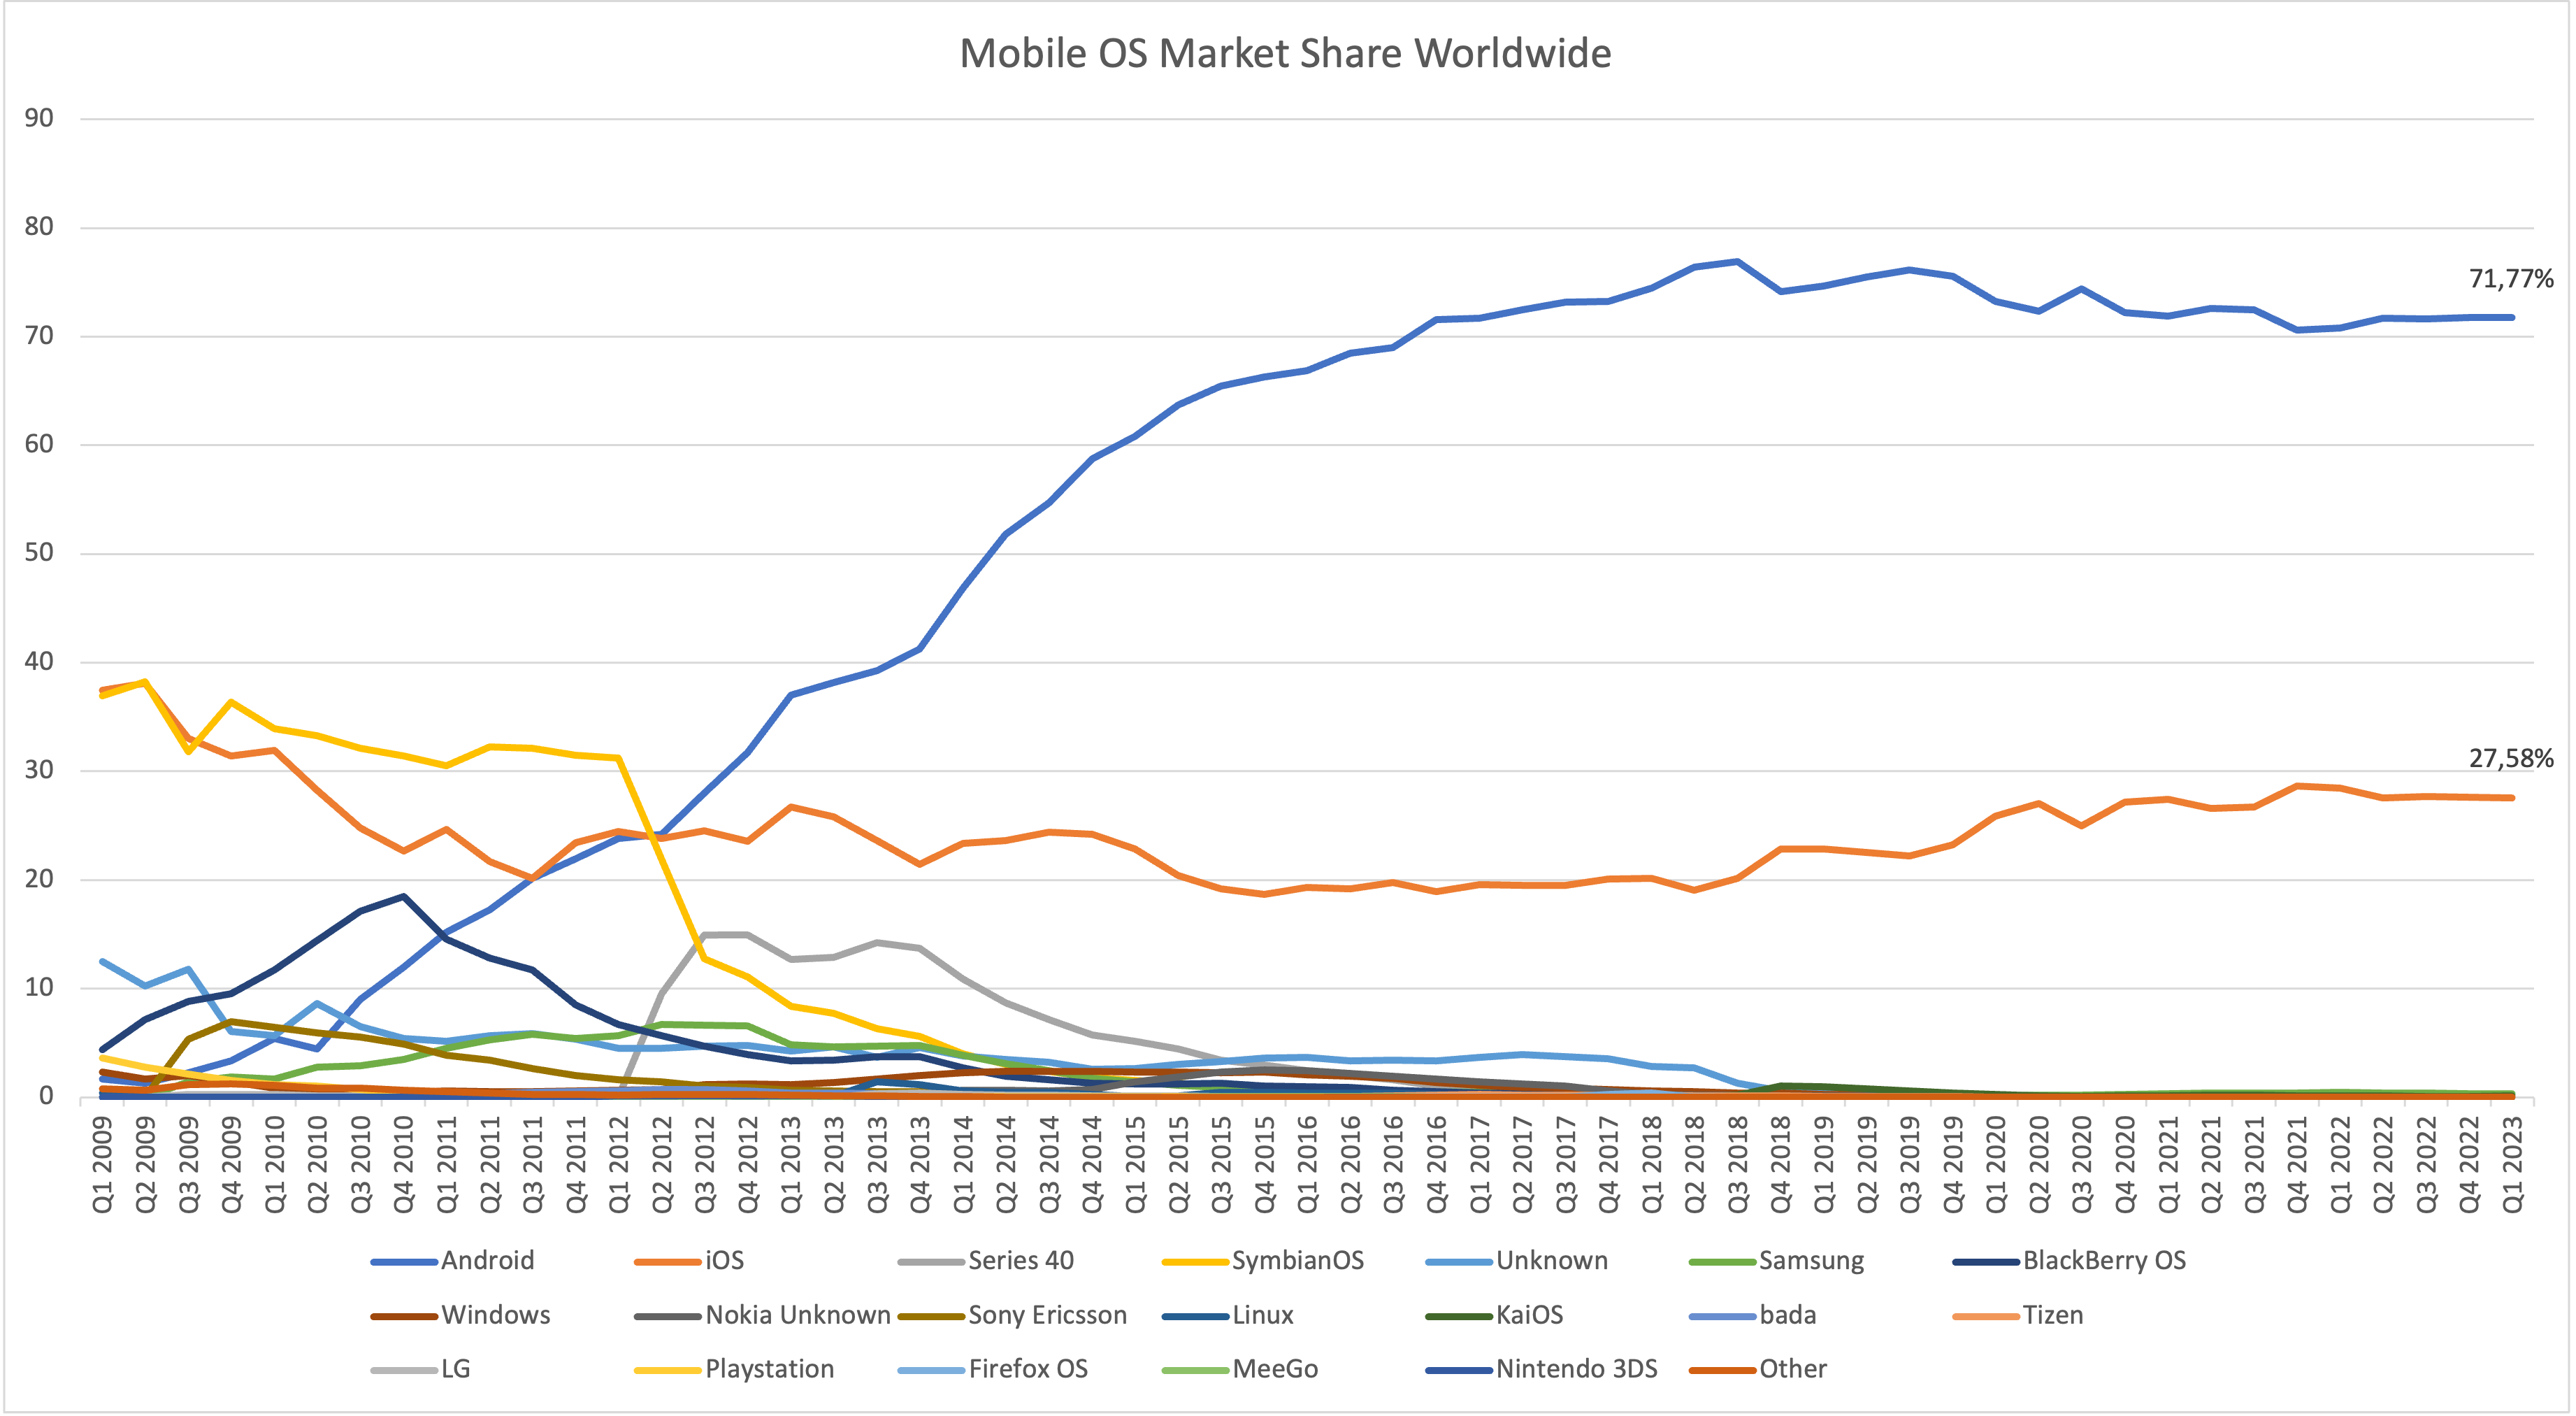
\includegraphics[width=\textwidth]{img/mobile_os_market}
  \caption{Mobile OS market (Source: Own work based on \cite{statcounter_mobile_os_market})}
  \label{fig:mobile_os_market}
\end{figure}

As can be seen in the Figure \ref{fig:ios_versions}, in case of iOS, almost 90\% of devices are running either the most or second-most recent major version of the operating system. Therefore, when targeting the Apple's system, probably a single codebase would be enough to guarantee the appropriate coverage.

However, in case of Android, there is a high level of market fragmentation, as nearly 20\% of smartphones or tablets are running older versions released as far as in 2015 (Figure \ref{fig:android_versions}). Because there are limitations such as deprecation of code commands and API (Application Programming Interfaces) behavior changes between distant versions, multiple codebases may be chosen to be maintained separately per a single mobile application. Another issue is the fact, that device manufacturers are able to apply various modifications to the operating system which can lead to errors occurring only on those devices \cite{comparison_technologies_multiplatform}, causing difficulties for developers. Because Apple is the exclusive manufacturer of devices running iOS, they do not suffer from such a problem. 

\begin{figure}[ht]
  \begin{minipage}{.47\textwidth}
    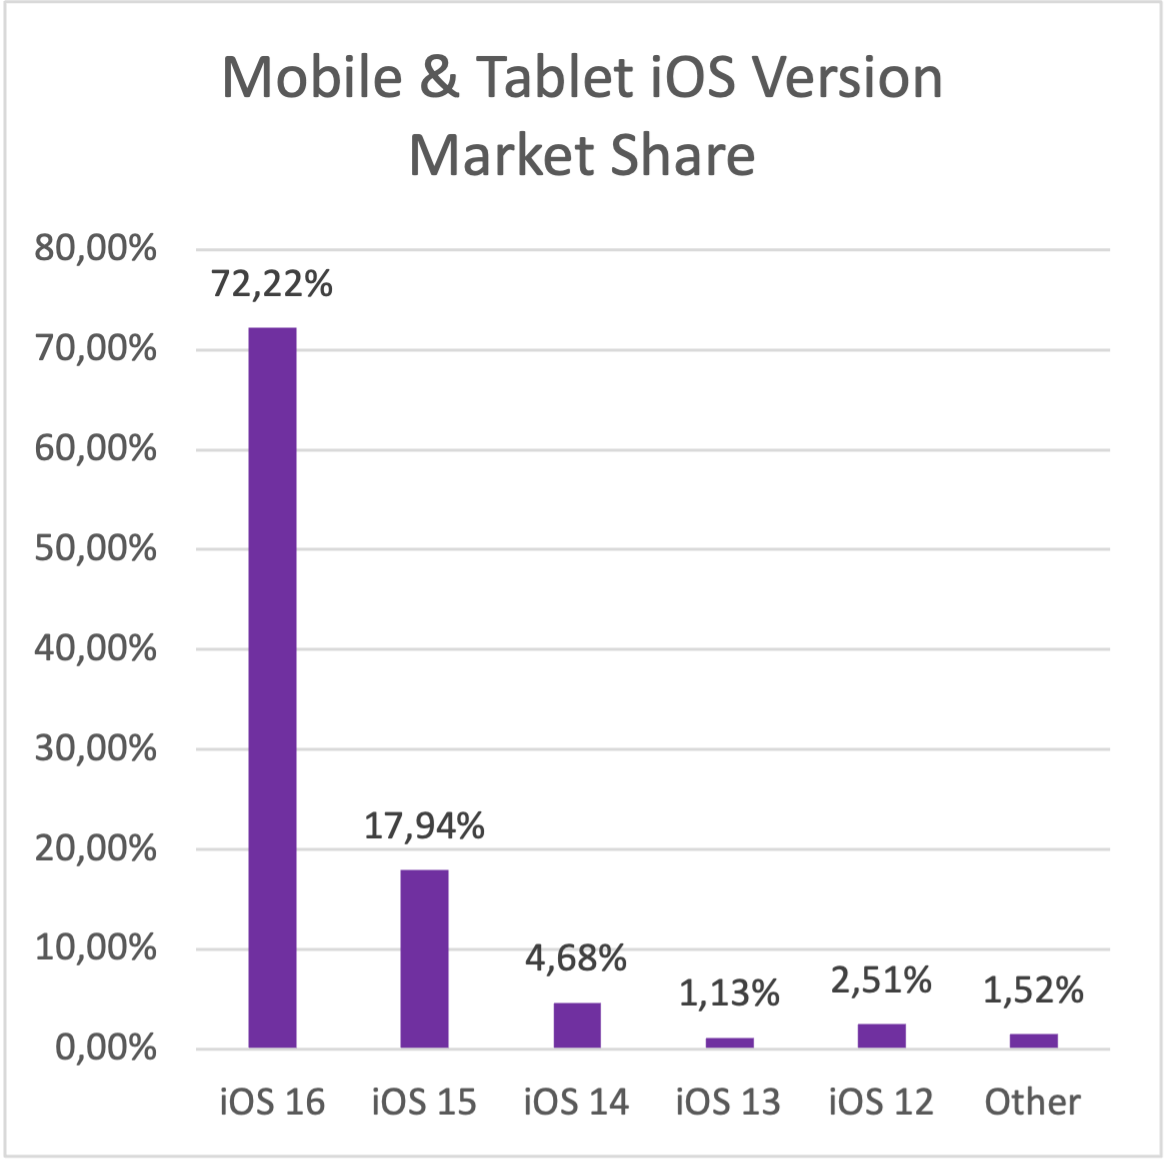
\includegraphics[width=\textwidth]{img/ios_ver_market_share}
    \caption{iOS version market share (Source: Own work based on \cite{statcounter_ios_version_market})}
    \label{fig:ios_versions}
  \end{minipage}
  \hfill
  \begin{minipage}{.47\textwidth}
    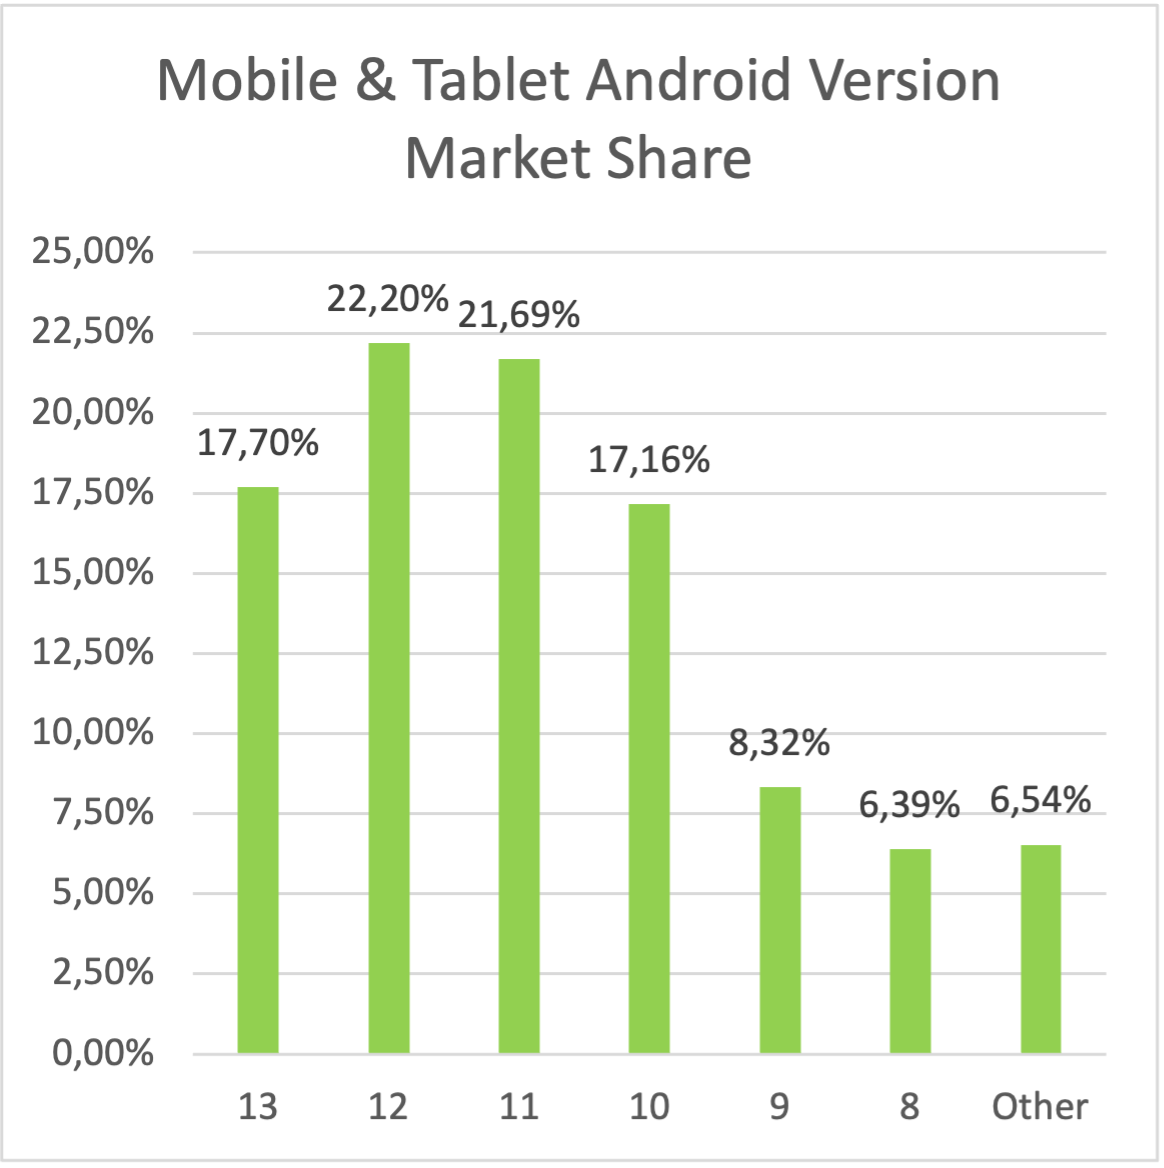
\includegraphics[width=\textwidth]{img/android_ver_market_share}
    \caption{Android version market share (Source: Own work based on \cite{statcounter_android_version_market})}
    \label{fig:android_versions}
  \end{minipage}
\end{figure}

\subsubsection{Android}

Android is an open-source operating system developed by the Open Handset Alliance and Google to run mainly on mobile devices such as smartphones and tablets but also TVs and cars \cite{android_what_is,comparison_technologies_multiplatform}. It is based on the Linux kernel and has a multiple-component structure \cite{android_architecture_and_application}, as can be seen in the Figure \ref{fig:android_architecture}. Each part takes responsibility for different tasks, e.g., Android Runtime provides optimized garbage collection and View System (included in Java API Framework) enables developers to implement the user interface layouts using various elements such as lists and buttons \cite{android_architecture}.

\begin{figure}[h]
    \centering
    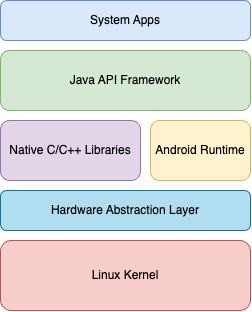
\includegraphics[scale=0.73]{img/android_architecture}
    \caption{Android architecture (Source: Own work based on \cite{android_architecture})}
    \label{fig:android_architecture}
\end{figure}

It is not necessary to use an IDEs (Integrated Development Environment) to build most software. Despite that, most programmers tend to reach out to them because of the guaranteed development comfort and productivity increase. Android Studio is the primary IDE for native mobile development of Android applications. It is created on top of IntelliJ's IDEA and provides numerous features such as Gradle, advanced debugging tools and profilers, etc \cite{android_studio_intro}.

For many years, Java has been the official language for Android development. However, since Google established Kotlin as the default choice in 2019 \cite{android_kotlin_first}, over 60\% of programmers have switched to it \cite{android_kotlin}. Furthermore, data shows that almost 90\% of the Google Play Store Top 500 USA mobile apps have been developed with it \cite{kc_kotlin_vs_java}. Kotlin's popularity is certainly going to grow in the upcoming years, considering the undeniable benefits it brings. Still, there are some scenarios in which Java could remain the first choice.

Table \ref{tab:java_kotlin_comparison} shows that all the features necessary for Android application development, such as e.g., Android SDK or AndroidX support, are fully provided by both Java and Kotlin. Furthermore, the latter introduces additional advantages in the form of enabling the usage of Jetpack Compose toolkit and even the ability to create multi-platform projects (Kotlin Multiplatform is currently only accessible in Beta version \cite{kotlin_multiplatform}).

\begin{table}[h]
  \centering
    \caption{Java and Kotlin comparison (Source: Own work based on \cite{android_kotlin_first})}
    \label{tab:java_kotlin_comparison}
    \begin{tabular}{ | p{55mm} | >{\centering}p{33mm} | >{\centering\arraybackslash}p{33mm} | }
      \hline
      \multicolumn{1}{ |c| }{\textbf{Feature}}&\textbf{Java}&\textbf{Kotlin}\\
      \hline
      Platform SDK support&Yes&Yes\\
      \hline
      Android Studio support&Yes&Yes\\
      \hline
      Lint&Yes&Yes\\
      \hline
      Guided docs support&Yes&Yes\\
      \hline
      API docs support&Yes&Yes\\
      \hline
      AndroidX support&Yes&Yes\\
      \hline
      AndroidX Kotlin-specific APIs (KTX, croutines, \dots)&N/A&Yes\\
      \hline
      Online training&Best effort&Yes\\
      \hline
      Samples&Best effort&Yes\\
      \hline
      Multi-platform projects&No&Yes\\
      \hline
      Jetpack Compose&No&Yes\\
      \hline
      Compiler plugin support&No&Yes (Kotlin Symbol Processing API)\\
      \hline
    \end{tabular}
\end{table}

Java is a high-level object-oriented programming language introduced as far back as 1995. It is one of the most popular languages in the world which is regularly updated, reaching major version 20 this year. However, in the context of Android development the supported versions are 8 and 11, with the latter requiring high Android API version in order to use all the offered elements (although upgraded API desugaring announced in February this year broadens the range of libraries available without increasing the app's minimum supported API level \cite{android_api_desugaring}). The advantages of Java mainly result from the fact it is present for a very long time. During the last 30 years it gathered a big community of developers with high-level experience. Therefore, it may be easier to form a competent team for the project. Moreover, there are numerous applications that had been created with Java which owners might not seek for a migration, which as a result maintains Java's importance in the market \cite{kc_kotlin_vs_java}.

On the other hand, Kotlin offers many assets because of which it has replaced Java as an official first-choice language for Android development, as mentioned before. Kotlin is a comparatively recent programming language introduced in 2016 by JetBrains. First and foremost, it is fully interoperable with Java and therefore, it is possible to call Kotlin code inside Java code and vice versa. Secondly, Kotlin's syntax is very concise and null-safe, thus increasing the speed of development and reducing the project's code lines and lowering the possibility of mistakes. For those reasons, implementation of new apps using Kotlin is fairly straight-forward and comfortable from the point of view of developers. Moreover, the migration of existing projects from Java to Kotlin is uncomplicated and can lead to size decrease and simplification of the codebase with much smaller Null Pointer Exception occurrence in runtime \cite{android_kotlin_first}.

Since Kotlin has already been established as the preferred programming language for Android development, all considerations in the scope of this thesis will be limited to it rather than Java.

One of the possibilities acquired when selecting Kotlin for Android development is the ability to use Jetpack Compose. It is a powerful toolkit used for building User Interface layouts introduced in 2021 with a goal improve that process compared to the previous XML approach \cite{android_jetpack_compose}. 
The main difference between the above-mentioned methods is the fact that they represent declarative and imperative approach, respectively. The former greatly reduces the amount of boilerplate code improving readibility as well as build time and therefore, increases development efficiency. Additionally, just as Kotlin offers interoperability with Java, Jetpack Compose provides the same in regards to XML. In short, XML approach implies the creation of layouts in XML markup files and later referencing them in the code while implementing the behavior. On the other hand, Jetpack Compose makes use of prebuilt components and intuitive state management \cite{jetpack_compose_vs_xml}. 

In order to improve the user experience accross different apps, Material design system was introduced by Google in 2014. First versions were strictly connected to Android only, however since then it has shifted towards being applicable for other platforms, including Web. Material provides detailed guidelines in the aspect of styling, accessibility, overall UX as well as prebuilt reusable UI components aiming to improve the efficiency of developing apps that are intuitive and responsive. The main principles are that every element of an app should be considered as a physical material and they should be combined together in layers while putting emphasis on natural animations and universal clarity. The big advantage of Material being applied in mobile apps is the fact that when a user understands how to use one it is automatically transposed onto others. On the other hand, an issue may be raised that if all the mobile apps available conformed to one design system, they would become overly monothematic and characterless \cite{material_design_get_started,material_design_pros_cons}.

\subsubsection{iOS}

iOS is the Apple's closed-source operating system based on Darwin OS that runs exclusively on Apple's smartphones (iPhones). It also lays beneath other mobile systems: iPadOS, tvOS and watchOS. It includes four layers that together enable the interaction between hardware and applications, as presented in Figure \ref{fig:ios_architecture}. Core OS layer provides necessary low-level services, e.g. Bluetooth, security and 64-bit support. Core Services layer incorporates multiple interfaces called Frameworks which are responsible for functionalities such as data management, cloud transfer and location. Media layer's task is to handle graphics and audio technology. Finally, Cocoa Touch enables user-application interaction, mainly through the implementation of touch gestures \cite{ios_architecture,mobile_os_survey}.

\begin{figure}[h]
  \centering
  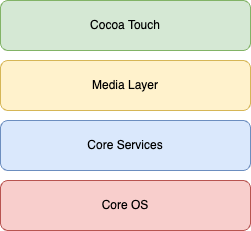
\includegraphics[scale=0.73]{img/ios_architecture}
  \caption{iOS architecture (Source: Own work based on \cite{ios_architecture})}
  \label{fig:ios_architecture}
\end{figure}

Xcode is the primary IDE for building iOS, iPadOS, watchOS, tvOS and macOS applications. It offers tools necessary for the whole range of development: implementation, testing, optimization and deployment. It includes Developer Tools, e.g. Simulator for testing, Instruments for performance profiling and Reality Composer for 3D and AR features \cite{xcode_documentation}. Native iOS development comes with additional costs compared to Android because Xcode requires a Mac device, e.g. the MacBook laptop, which itself can be expensive especially when considering a large development team \cite{comparison_technologies_multiplatform,comp_study_hybrid}.

Currently, the officially recommended programming language for iOS development is Swift. It was introduced with the goal to replace previously used Objective-C. Essentially, it was supposed to increase the ease of development and maintenance of the codebase, make it more error-proof and performant. Objective-C remains supported by Apple for the indefinite future, however since 2011, it has not received any major updates staying at version 2.0 \cite{swift_overview,speed_performance_swift_objective_c,swift_vs_objective_c,wiki_objective_c}.

Objective-C is an object-oriented, dynamically-typed programming language published in 1984. Similarly to Java for Android development, Objective-C is very stable because of its age and is still necessary for legacy applications support because Swift does not allow development of applications for lower than 7.0 version of iOS. Additionally, it allows Swift code usage by automatically regenerating files to enable the integration, which makes it possible to keep the existing code in old projects even when migrating to Swift \cite{swift_objective_c_new_language,geeks_objective_c_swift}.

Swift is a compiled, statically-typed programming language introduced by Apple in 2014. It holds the features of Objective-C while providing various improvements such as automatic memory management (ARC). Its syntax is much more concise, resulting in readable and easily maintainable code, as well as quicker development time. It was emphasized on release that Swift increases safety and it does so by overflow checking, optionals, type safety, etc. Furthermore, Swift has been shown to run faster than Objective-C. It is also fully interoperable with Objective-C code \cite{swift_overview,swift_objective_c_new_language,geeks_objective_c_swift}. However, one of the issues is differences between iOS versions that may force code rewriting. Finally, an important advantage of Swift is that it enables the usage of SwiftUI \cite{comparison_technologies_multiplatform}.

In iOS development, there are multiple ways to implement user interface views. Apple offers two design solutions which can be used together if needed: UIKit and the more recent SwiftUI. The latter has been acknowledged by Apple to be the primary solution \cite{comparison_technologies_multiplatform}. UIKit is an imperative framework that can be applied programmatically (imperatively) or by using Interface Builder to create XIBs (XML Interface Builder) or Storyboards, while SwiftUI is a declarative framework. The difference in programming paradigms results in less code lines necessary for the same task when programming with SwiftUI. Furthermore, SwiftUI apps can be built for all platforms of Apple devices, while UIKit is meant only for iOS, iPadOS and tvOS and requires AppKit and WatchKit to support the rest. On the other hand, SwiftUI supports iOS version 13.0 minimum so if further backwards compatibility is needed than UIKit remains the first choice \cite{swiftui_overview,xib_why_use,swiftui_uikit}.

In order to provide consistency among different applications and across different Apple platforms, Human Interface Guidelines (HIG) has been introduced. It is a document containing detailed general and platform-specific design principles and practices. Developing applications according to that information helps guarantee that the end product is in accordance with Apple's standard, both visually and behaviorally. Consequently, great user experience is reached as users can easily comprehend applications that are similar and consistent with the platform they are used to, e.g. the positioning of action buttons and touch gestures in iOS apps. Exemplary aspects underlined in HIG are layout creation, navigation, inputs, accessibility, technology support and more \cite{hig_overview}.

\subsubsection{Web development in relation to native mobile development}

While solely native mobile development has been considered in this chapter, it is important to reflect upon its connection to web development. Of course, it is a possibility that a service is designed to be available exclusively in the form of a mobile application and such attitude will remain unchanged in the future. However, there are some reasons for which a publisher may look to extend the supported platform list after time. For instance, a small service may start as an Android application and grow enough to need other platforms in order to reach a bigger volume of users. In such a case, iOS support may be added as well as a website may be developed. The second option is especially probable as it provides accessibility for all platforms. The fact that such a service launched in the shape of a single-platform application in the first place may be caused by many aspects, such as dictated functional requirements, detachment or overlook during the initial planning stages as well as market trends analysis \cite{web_mobile_app}. Cross-platform frameworks could be the answer to the above-mentioned issues.


% !TEX encoding = UTF-8 Unicode 
% !TEX root = praca.tex

\subsection{Cross-platform mobile development}

Most cross-platform frameworks require a middle layer that connects the app with the system and translates the commands to be natively called. This is considered to be a possible root of performance decrease \cite{appdynamics_mobile_app_performance}.

\subsubsection{Flutter}



\subsubsection{React Native}



\subsubsection{Ionic}



\subsubsection{Comparison}

\begin{table}[hb]
	\centering
    \caption{Cross-platform frameworks comparison (Source: Own work based on \dots)}
    \label{tab:framework_comparison}
	\begin{tabular}{ |l|p{30mm}|p{30mm}|p{30mm}| }
		\hline
        \diagbox{Element}{Framework} & Flutter & React Native & Ionic \\
		\hline
		Initial release&2017&&\\
        \hline
		Current stable version&&&\\
        \hline
		Implemented with&C, C++, Dart&&\\
        \hline
		Supported platforms&Android, iOS, Web, Windows, macOS, Linux&&\\
        \hline
		Supported IDEs??&&&\\
        \hline
		Programming language&Dart&&\\
        \hline
		Rendering&Canvas drawing&Native platform components&Native platform components\\
		\hline
	\end{tabular}
\end{table}


% !TEX encoding = UTF-8 Unicode 
% !TEX root = praca.tex

\section{Evaluation of cross-platform frameworks}


% !TEX encoding = UTF-8 Unicode 
% !TEX root = praca.tex

\section{Performance measurement}

\subsection{Mobile development}

\subsection{Web development}


% \begin{equation}
% 	\sum_{i=1}^{\infty}a_i
% 	\label{eq:myEquation}
% \end{equation}

% % replace {c} with the appropriate language
% \begin{listing}
% 	\begin{minted}{c}  
% int main()
% {
%    int a=2*3;
%    printf("**Ala ma kota\n**");
%    while(!I2C_CheckEvent(I2C1, I2C_EVENT_MASTER_MODE_SELECT)); /* EV5 */
%    return 0;
% }
% \end{minted}
% 	\caption{C language} \label{listing:myListing}
% \end{listing}


% !TEX encoding = UTF-8 Unicode 
% !TEX root = praca.tex

\chapter{Research method}

\section{Performance metrics}

\subsection{Mobile environment}

\subsection{Web environment}

\section{Research scenarios}

\section{Testing tools}

\subsection{Mobile environment}

\subsection{Web environment}

\section{Testing devices}

% !TEX encoding = UTF-8 Unicode 
% !TEX root = praca.tex

\chapter{Mobile application performance measurement}\label{chap:app_performance}

Application performance can be analyzed differently depending on the defined context. It is usually performed during the implementation, testing and maintainance phases present in the general software development cycle. In this chapter, the importance of app performance measurement is ephasized and exemplary metrics are explained separately for mobile and web developement.

The possibility to install and uninstall mobile apps within seconds directly affects the commercial mobile app market. In order to compete, publishers need to make sure they provide their services at the highest quality acquirable so that users don't turn to the competitor's solution. Almost 30\% of consumers instantly switch to other available products if their needs are not satisfied. App performance is considered to be one of the more important aspects in this context, as 70\% of users perform an immediate switch solely based on loading time being too long. For that reason, no matter how big or successful, each mobile app publisher must not underestimate the importance of performance offered by their product \cite{micro_moments_guide}. 

Mobile app performance is a broad term and can be understood differently and described with higher or lower level of detail. It can be seen as only dependent on consumers' impressions. The main aspects of app performance as perceived by users are device resource usage, smoothness, loading times, app size etc. On the other hand, considering app performance from the publisher's perspective includes additional metrics, e.g., user return rate and crash occurrence frequency.

\begin{longtblr}[
    caption = {Selected app performance metrics from the perspective of user experience (Source: Own work based on \cite{appdynamics_mobile_app_performance,saborido_app_performance_optimization,willocx_quantative_perf})},
    label = {tab:performance_ux},
]{ colspec = { |l|X| }, hlines} 
    \textbf{Metric}&\textbf{Description}\\
    CPU usage&Measures the percentage of CPU capacity utilized by the running application. Suboptimal source code and heavy computations may cause high CPU usage which negatively affects user experience.\\
    Memory consumption&Measures the amount of RAM consumed by the running application. It is especially significant when considering low-end devices with very little memory available. High memory usage results with fewer apps being able to run at the same time on a device. This metric is used to find and fix potential memory leaks.\\
    Power consumption&Measures the amount of energy consumed by the running application. It is usually directly related to other metrics, especially CPU usage, because heavy load on CPU is one of the biggest causes for battery drain.\\
    Smoothness&Measures the frame rate in FPS (Frames Per Second). The higher the frame rate, the higher the perceived smoothness of the app. 60 FPS is considered to be an indicator of a frame rate providing very good user experience. Furthermore, the frame rate should remain as stable as possible during the app use.\\
    Loading times&There are numerous types of loading times measurement. First and foremost, the app's launch time can be considered but also the times of navigation, page load, computation, etc. These are the metrics highly impacting the user's perception of app performance.\\
    App size&Consists of two measures: the storage space used by the installed application, as well as the size of the installer itself. It is especially important for low-end devices.\\
\end{longtblr}

\begin{longtblr}[
    caption = {Selected app performance metrics from the perspective of publisher (Source: Own work based on \cite{appsamurai_app_performance,khandelwal_load_testing,smartlook_performance_kpis})},
    label = {tab:performance_publisher},
]{ colspec = { |l|X| }, hlines} 
    \textbf{Metric}&\textbf{Description}\\
    Load handling&Load testing is an important part of the performance measurement. The goal is to simulate a very high user count at once. The outcome helps to find potential performance issues and bottlenecks in critical scenarios and thus, optimize the app scalability. Load testing is usually performed with specialized tools automating the process.\\
    Total and new users count&These metrics represent the popularity of the app. User count should be monitored in relation to issue occurrence in order to make sure the app is scalable.\\
    Crash-free users percentage&Measures the frequency of crash occurrence among the user base. Should be considered of high priority and monitored regularly, especially after new app features introduction.\\
    User return rate&Valuable metric used to detect existence of issues leading to user dissatisfaction resulting in abandoning the app. Calculated as the number of user sessions during a time period.\\
    Revenue&Measures the sales connected to the app. It is important in relation to Return Of Investment. It is helpful with analyzing effectiveness of marketing strategies applied.\\
    User satisfaction&Metric based on ratings and surveys. Should be monitored in order to discover existence of functional and performance issues.\\
\end{longtblr}

Table \ref{tab:performance_ux} contains an overview of the major application performance metrics understood to be related to user experience. Per contra, Table \ref{tab:performance_publisher} provides descriptions for some of the metrics considered important from the perspective of the app publisher. As can be observed, app performance can be viewed in different ways depending on the context, e.g. business or technical.

\clearpage


% !TEX encoding = UTF-8 Unicode 
% !TEX root = praca.tex

\chapter{Research method}

\section{Performance metrics}

\subsection{Mobile environment}

\subsection{Web environment}

\section{Research scenarios}

\section{Testing tools}

\subsection{Mobile environment}

\subsection{Web environment}

\section{Testing devices}

% !TEX encoding = UTF-8 Unicode 
% !TEX root = praca.tex

\chapter{Implementation of sample applications}

In this chapter, the development of the sample applications is presented. The implementation is based on the research scenarios defined in chapter \ref{chap:research_scenarios}.

\section{Research scenario 1: List scrolling and filtering}

The application consists of two main elements: a \emph{Switch} and a \emph{List}. Toggling the \emph{Switch} applies filtering (only every 6th element remains). The \emph{List} is generated automatically with 10000 elements and is scrollable. The optimal components (e.g. Flutter's \emph{ListView.builder}) have been chosen per each technology, therefore only visible items are rendered.

\begin{figure}[H]
    \begin{minipage}{.47\textwidth}
      \centering
      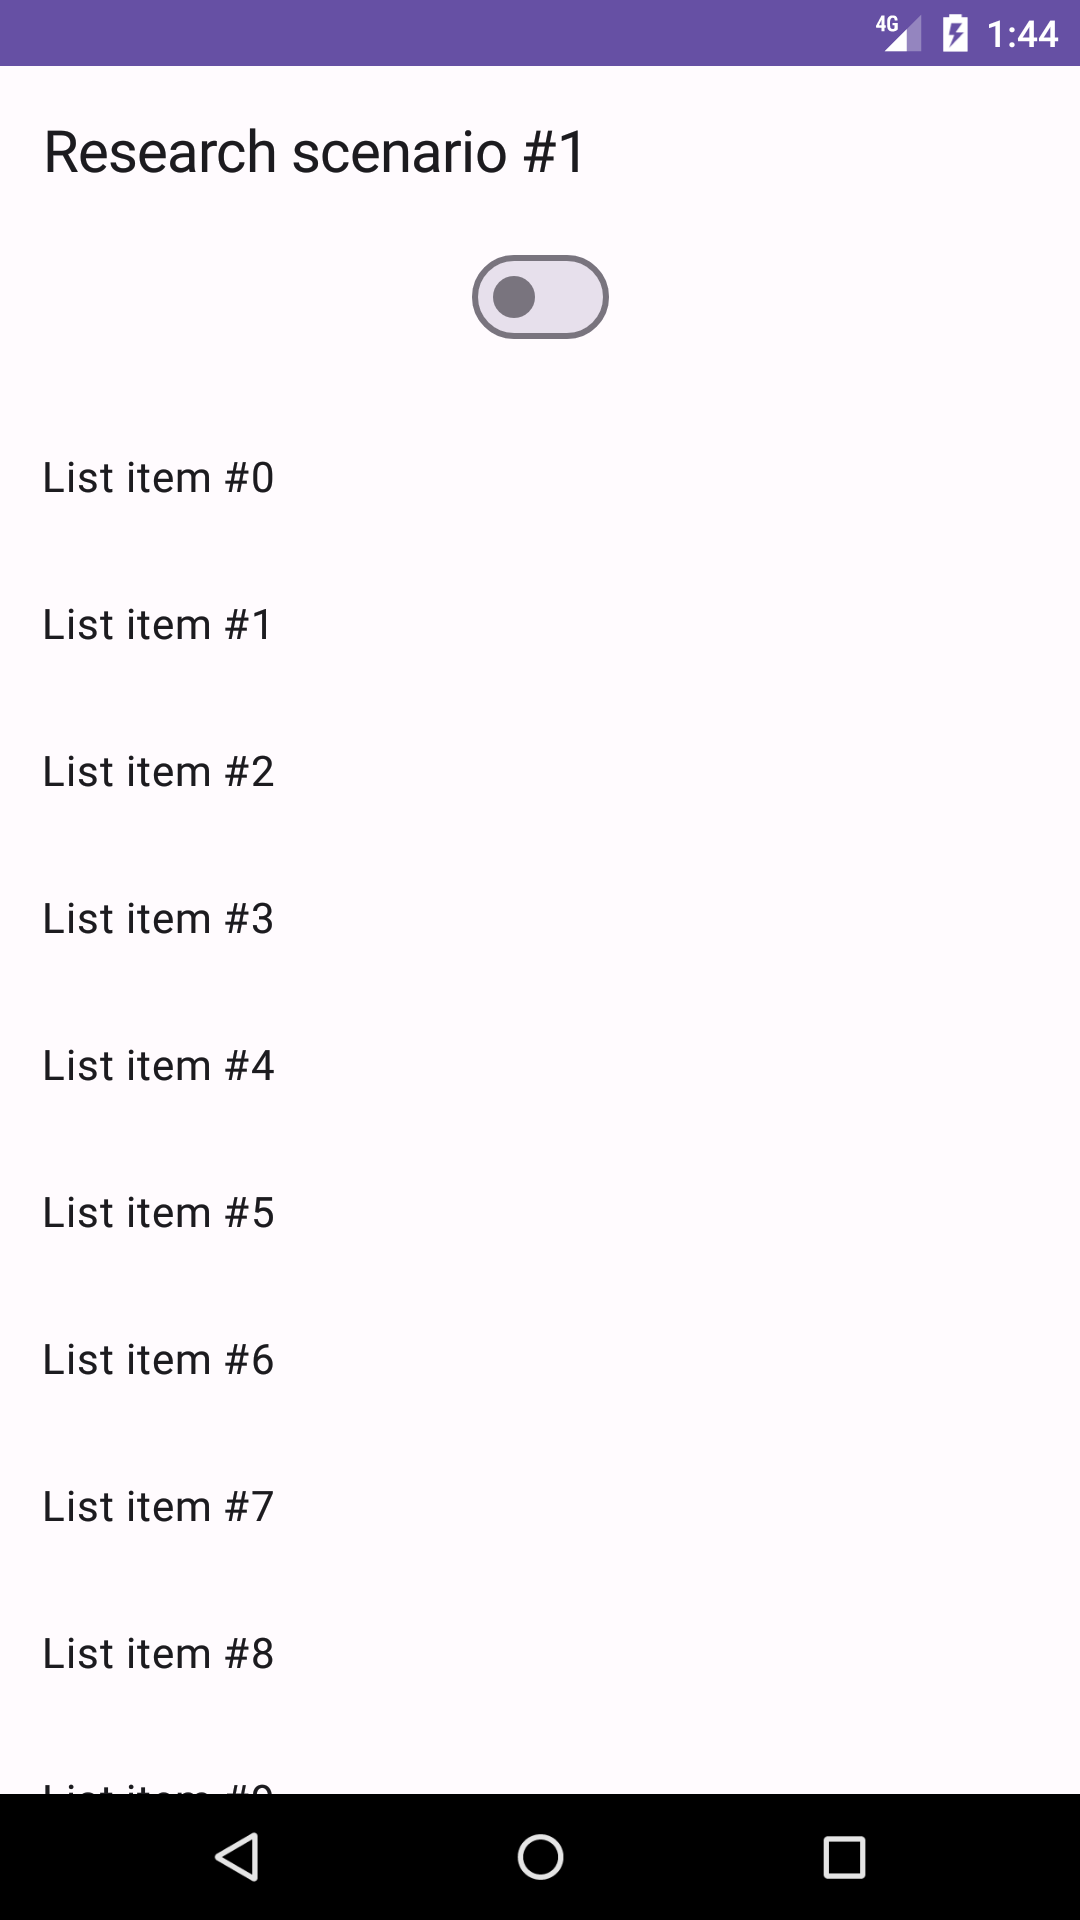
\includegraphics[height=50mm]{img/app1_kotlin}
      \caption{App 1: Kotlin (Source: Own work)}
      \label{fig:app1_kotlin}
    \end{minipage}
    \hfill
    \begin{minipage}{.47\textwidth}
      \centering
      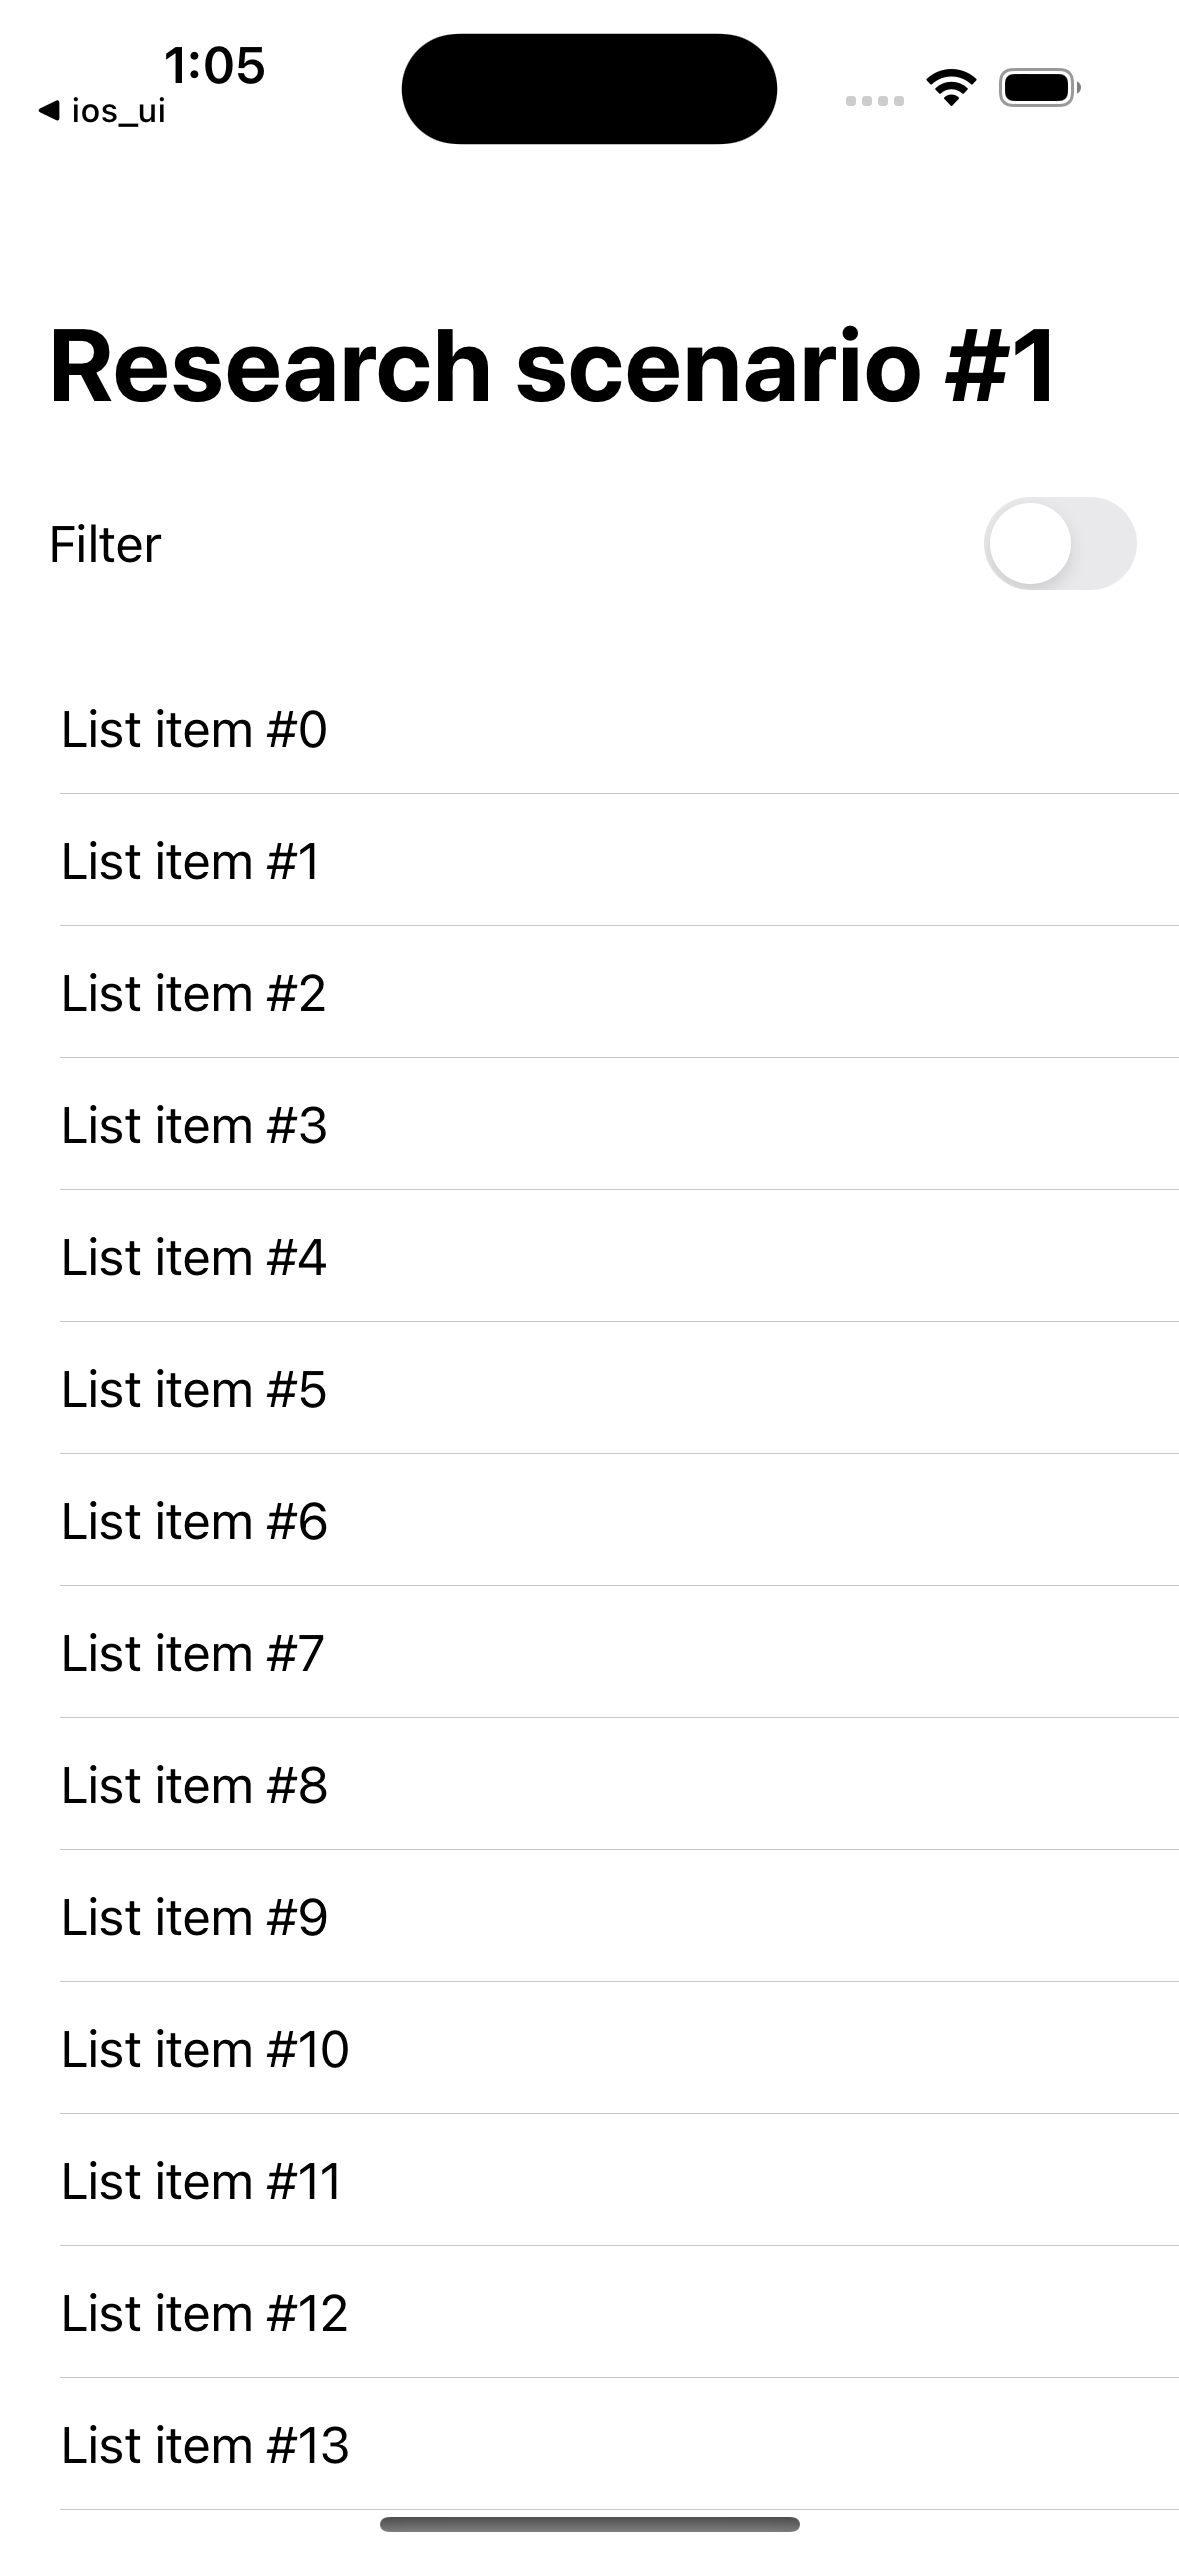
\includegraphics[height=50mm]{img/app1_swift}
      \caption{App 1: Swift (Source: Own work)}
      \label{fig:app1_swift}
    \end{minipage}
\end{figure}

\begin{figure}[H]
  \begin{minipage}{.47\textwidth}
    \centering
    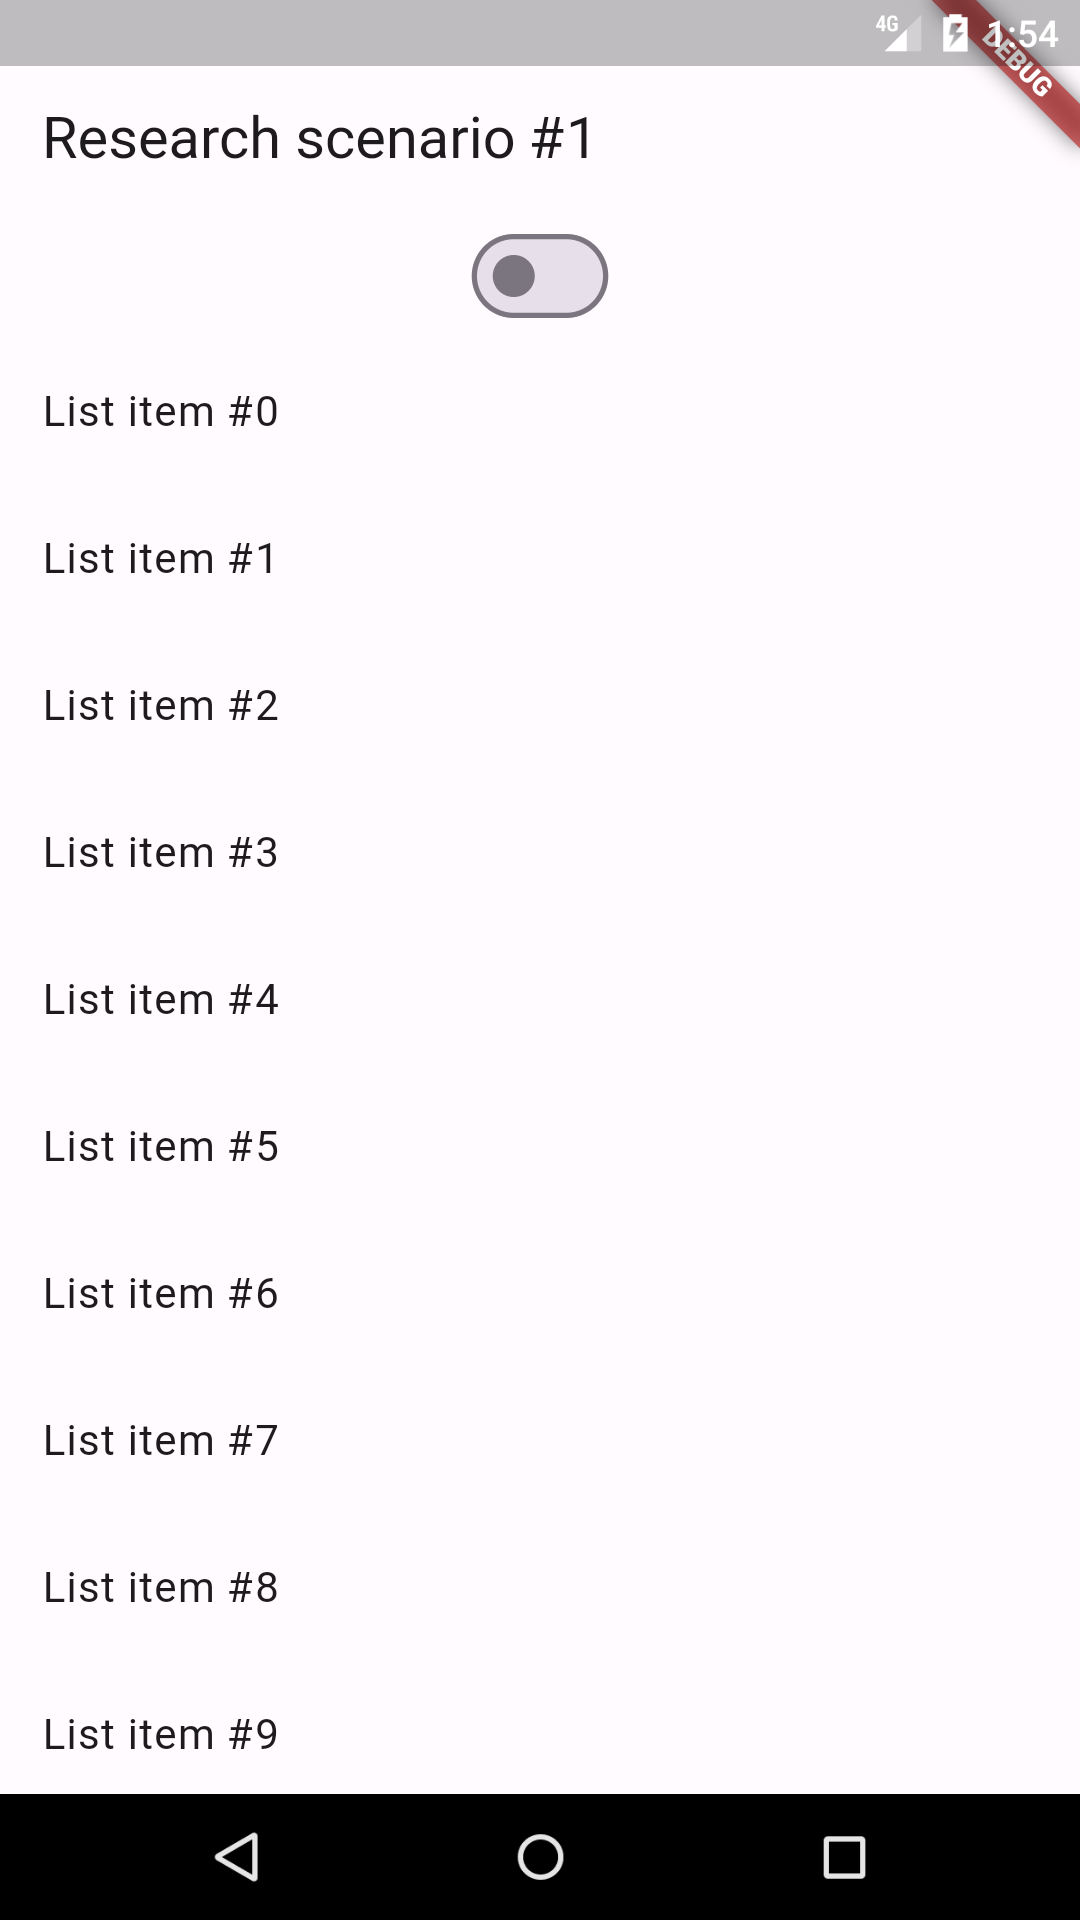
\includegraphics[height=50mm]{img/app1_flutter_android}
    \caption{App 1: Flutter Android (Source: Own work)}
    \label{fig:app1_flutter_android}
  \end{minipage}
  \hfill
  \begin{minipage}{.47\textwidth}
    \centering
    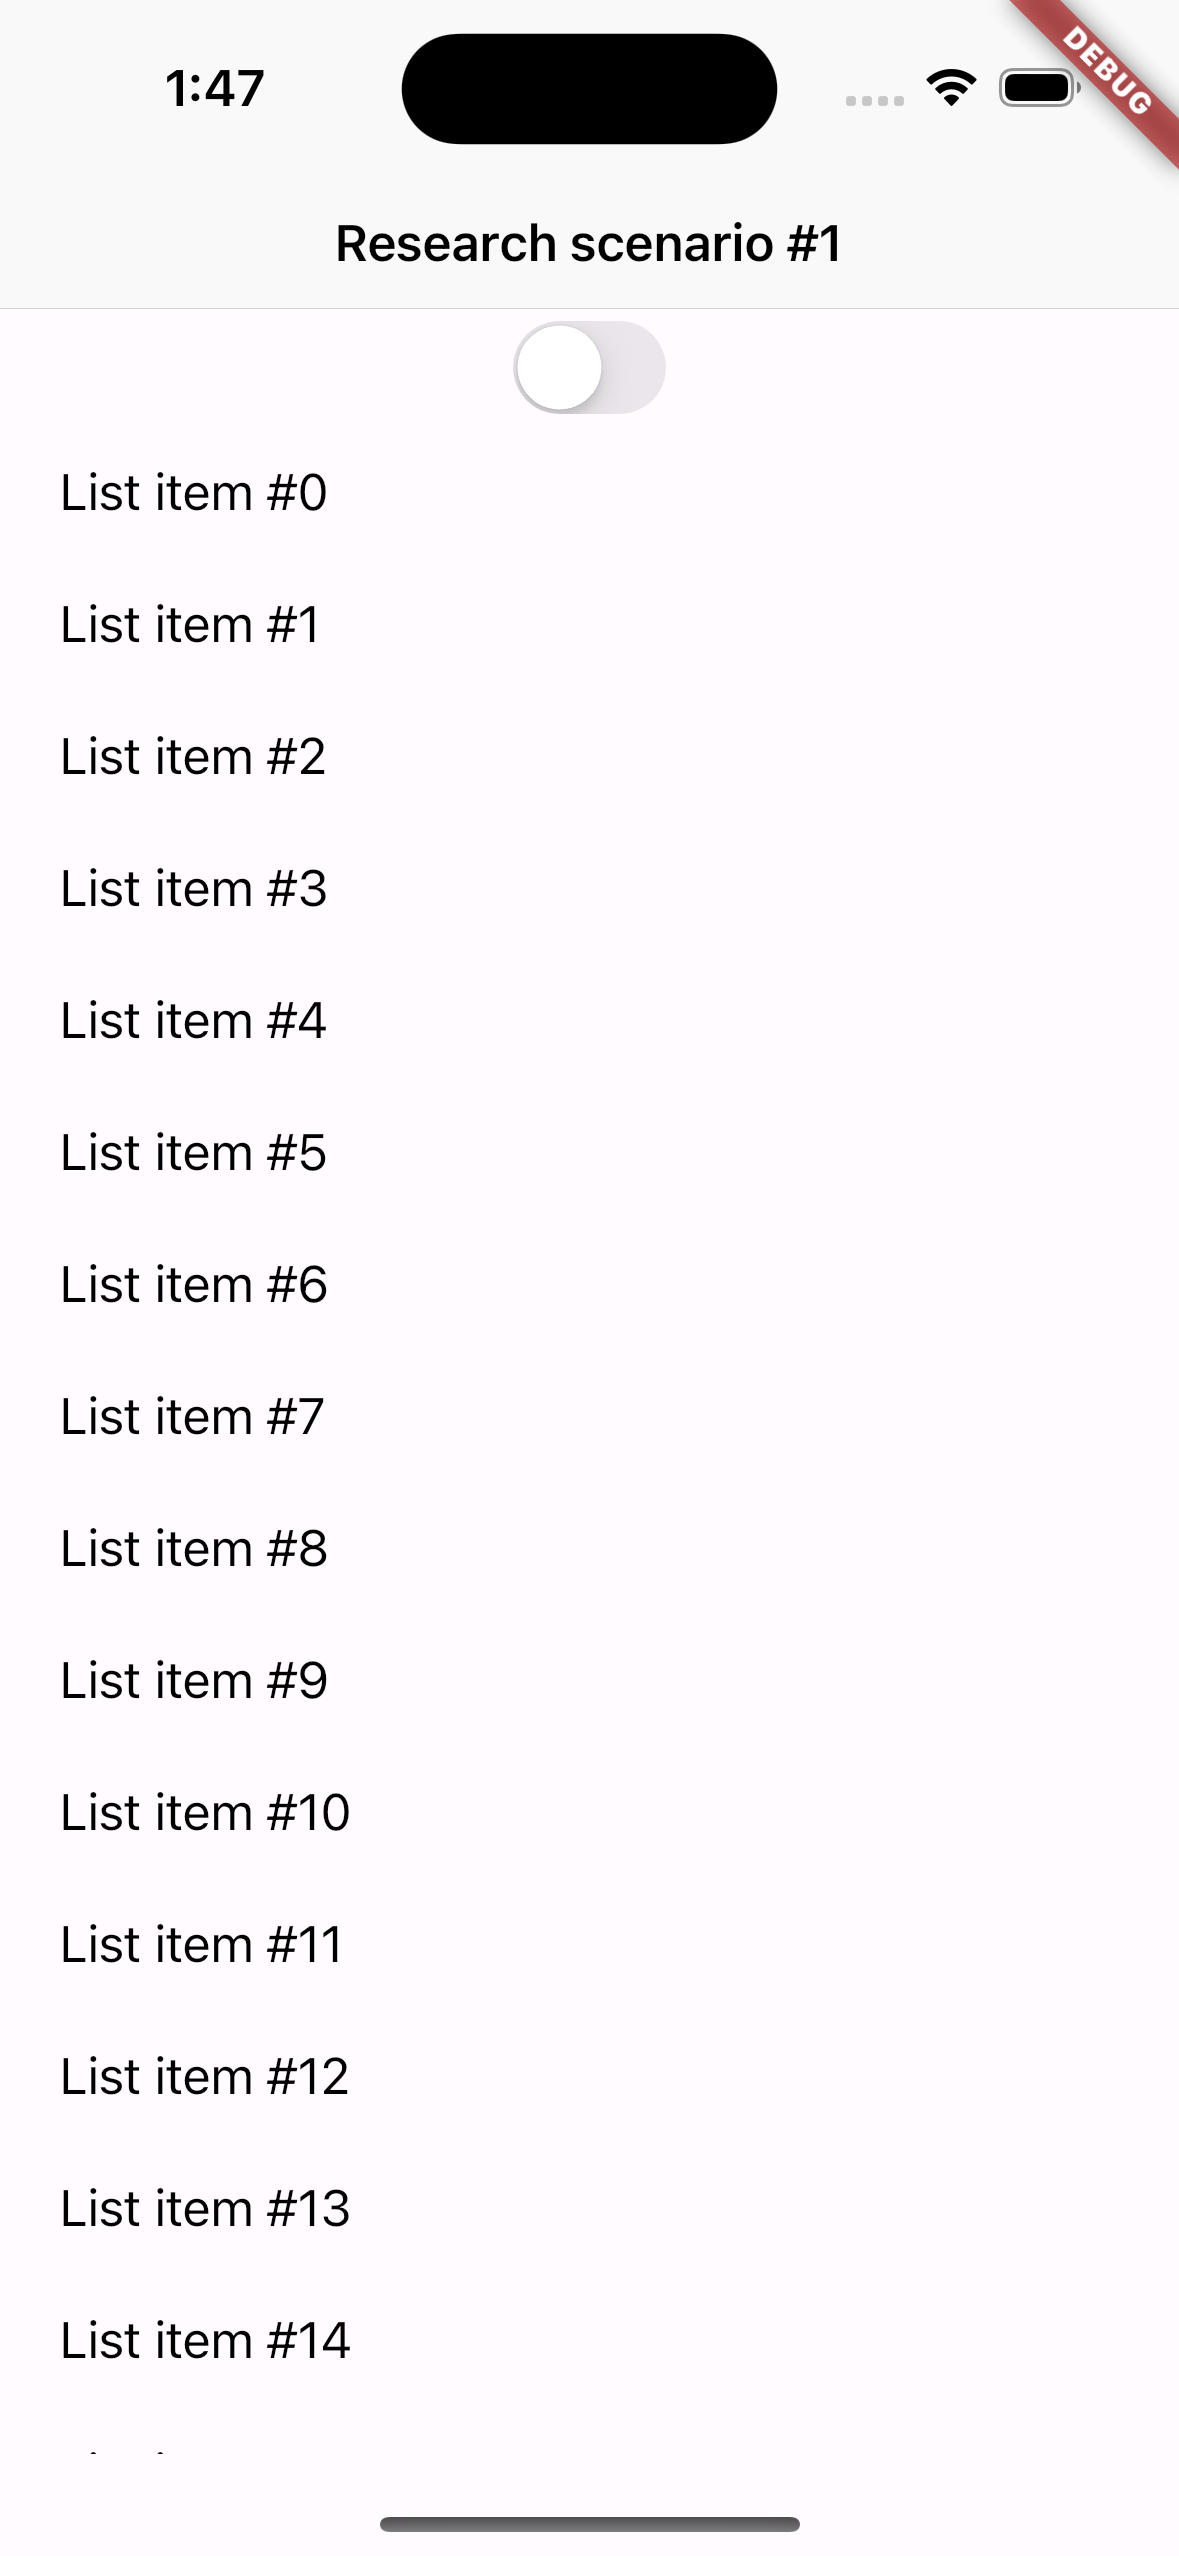
\includegraphics[height=50mm]{img/app1_flutter_ios}
    \caption{App 1: Flutter iOS (Source: Own work)}
    \label{fig:app1_flutter_ios}
  \end{minipage}
\end{figure}

\begin{figure}[H]
  \begin{minipage}{.47\textwidth}
    \centering
    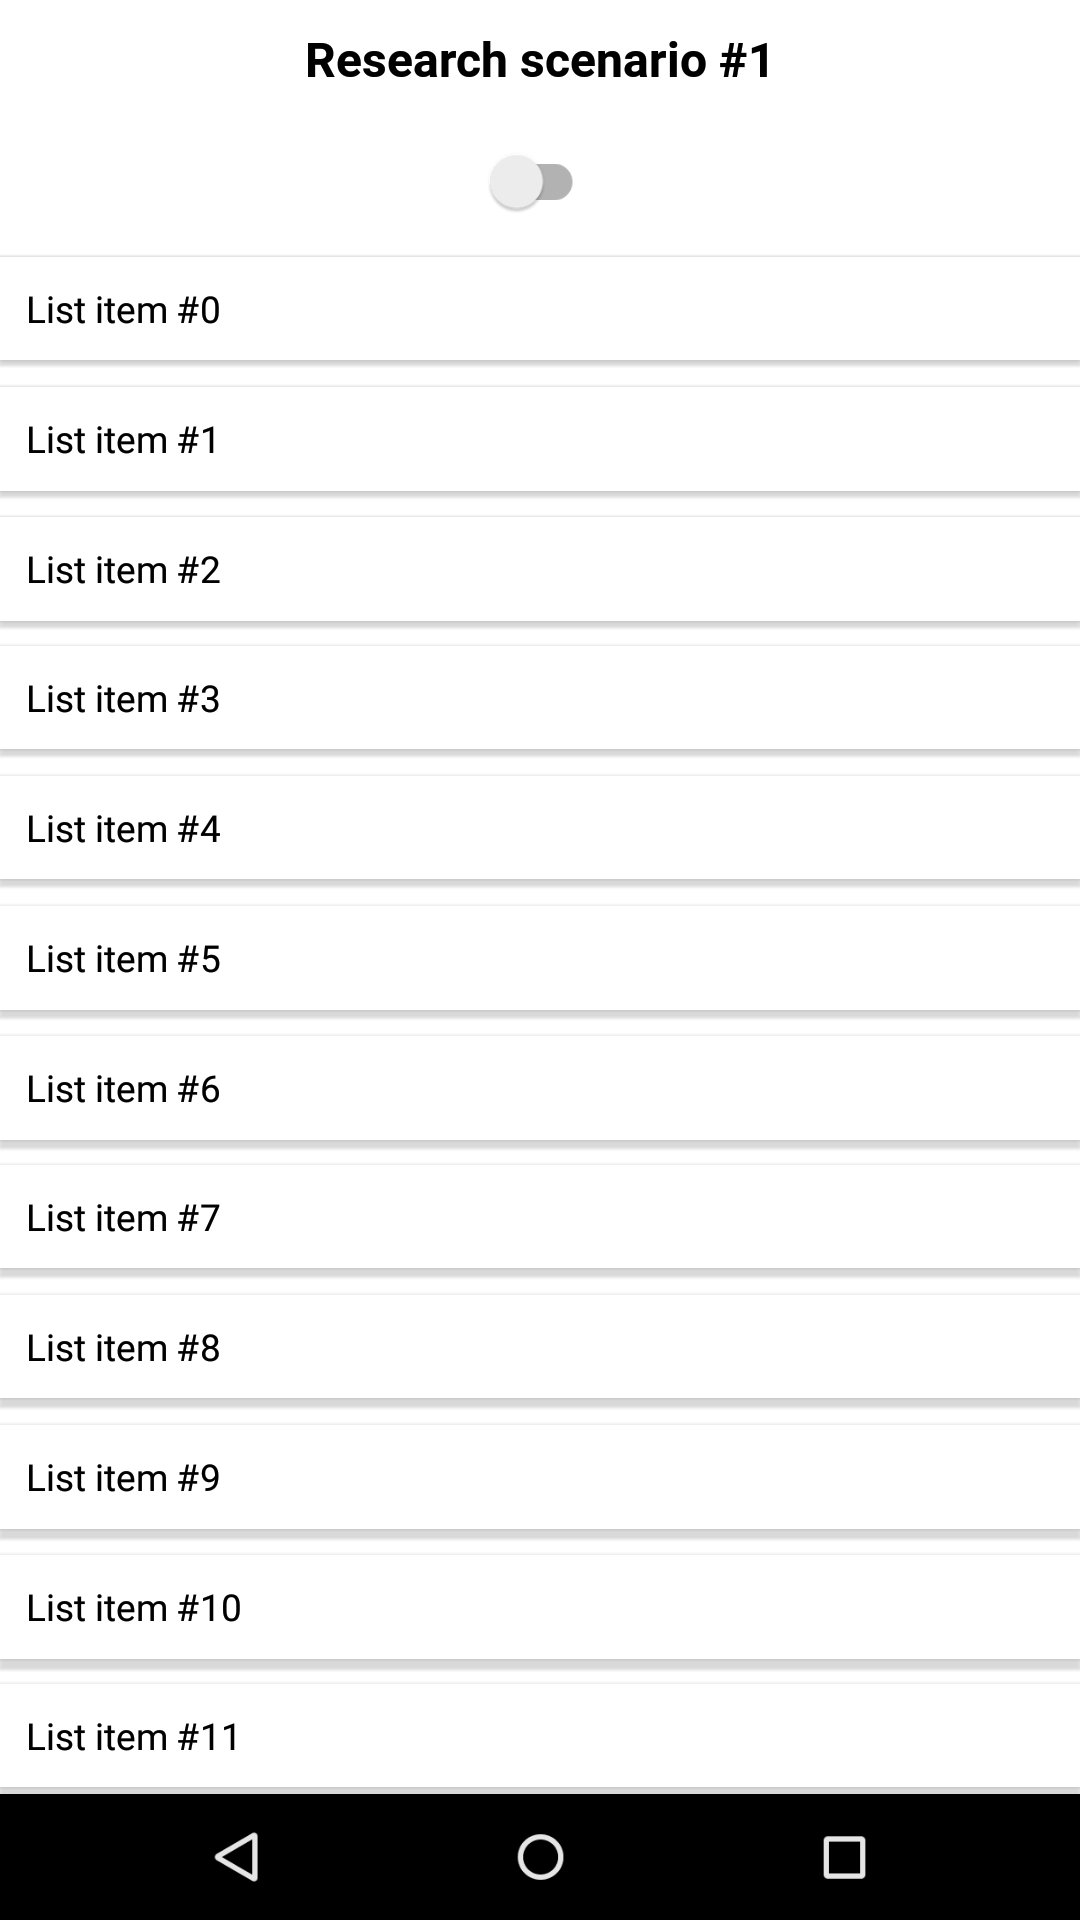
\includegraphics[height=50mm]{img/app1_rn_android}
    \caption{App 1: React Native Android (Source: Own work)}
    \label{fig:app1_rn_android}
  \end{minipage}
  \hfill
  \begin{minipage}{.47\textwidth}
    \centering
    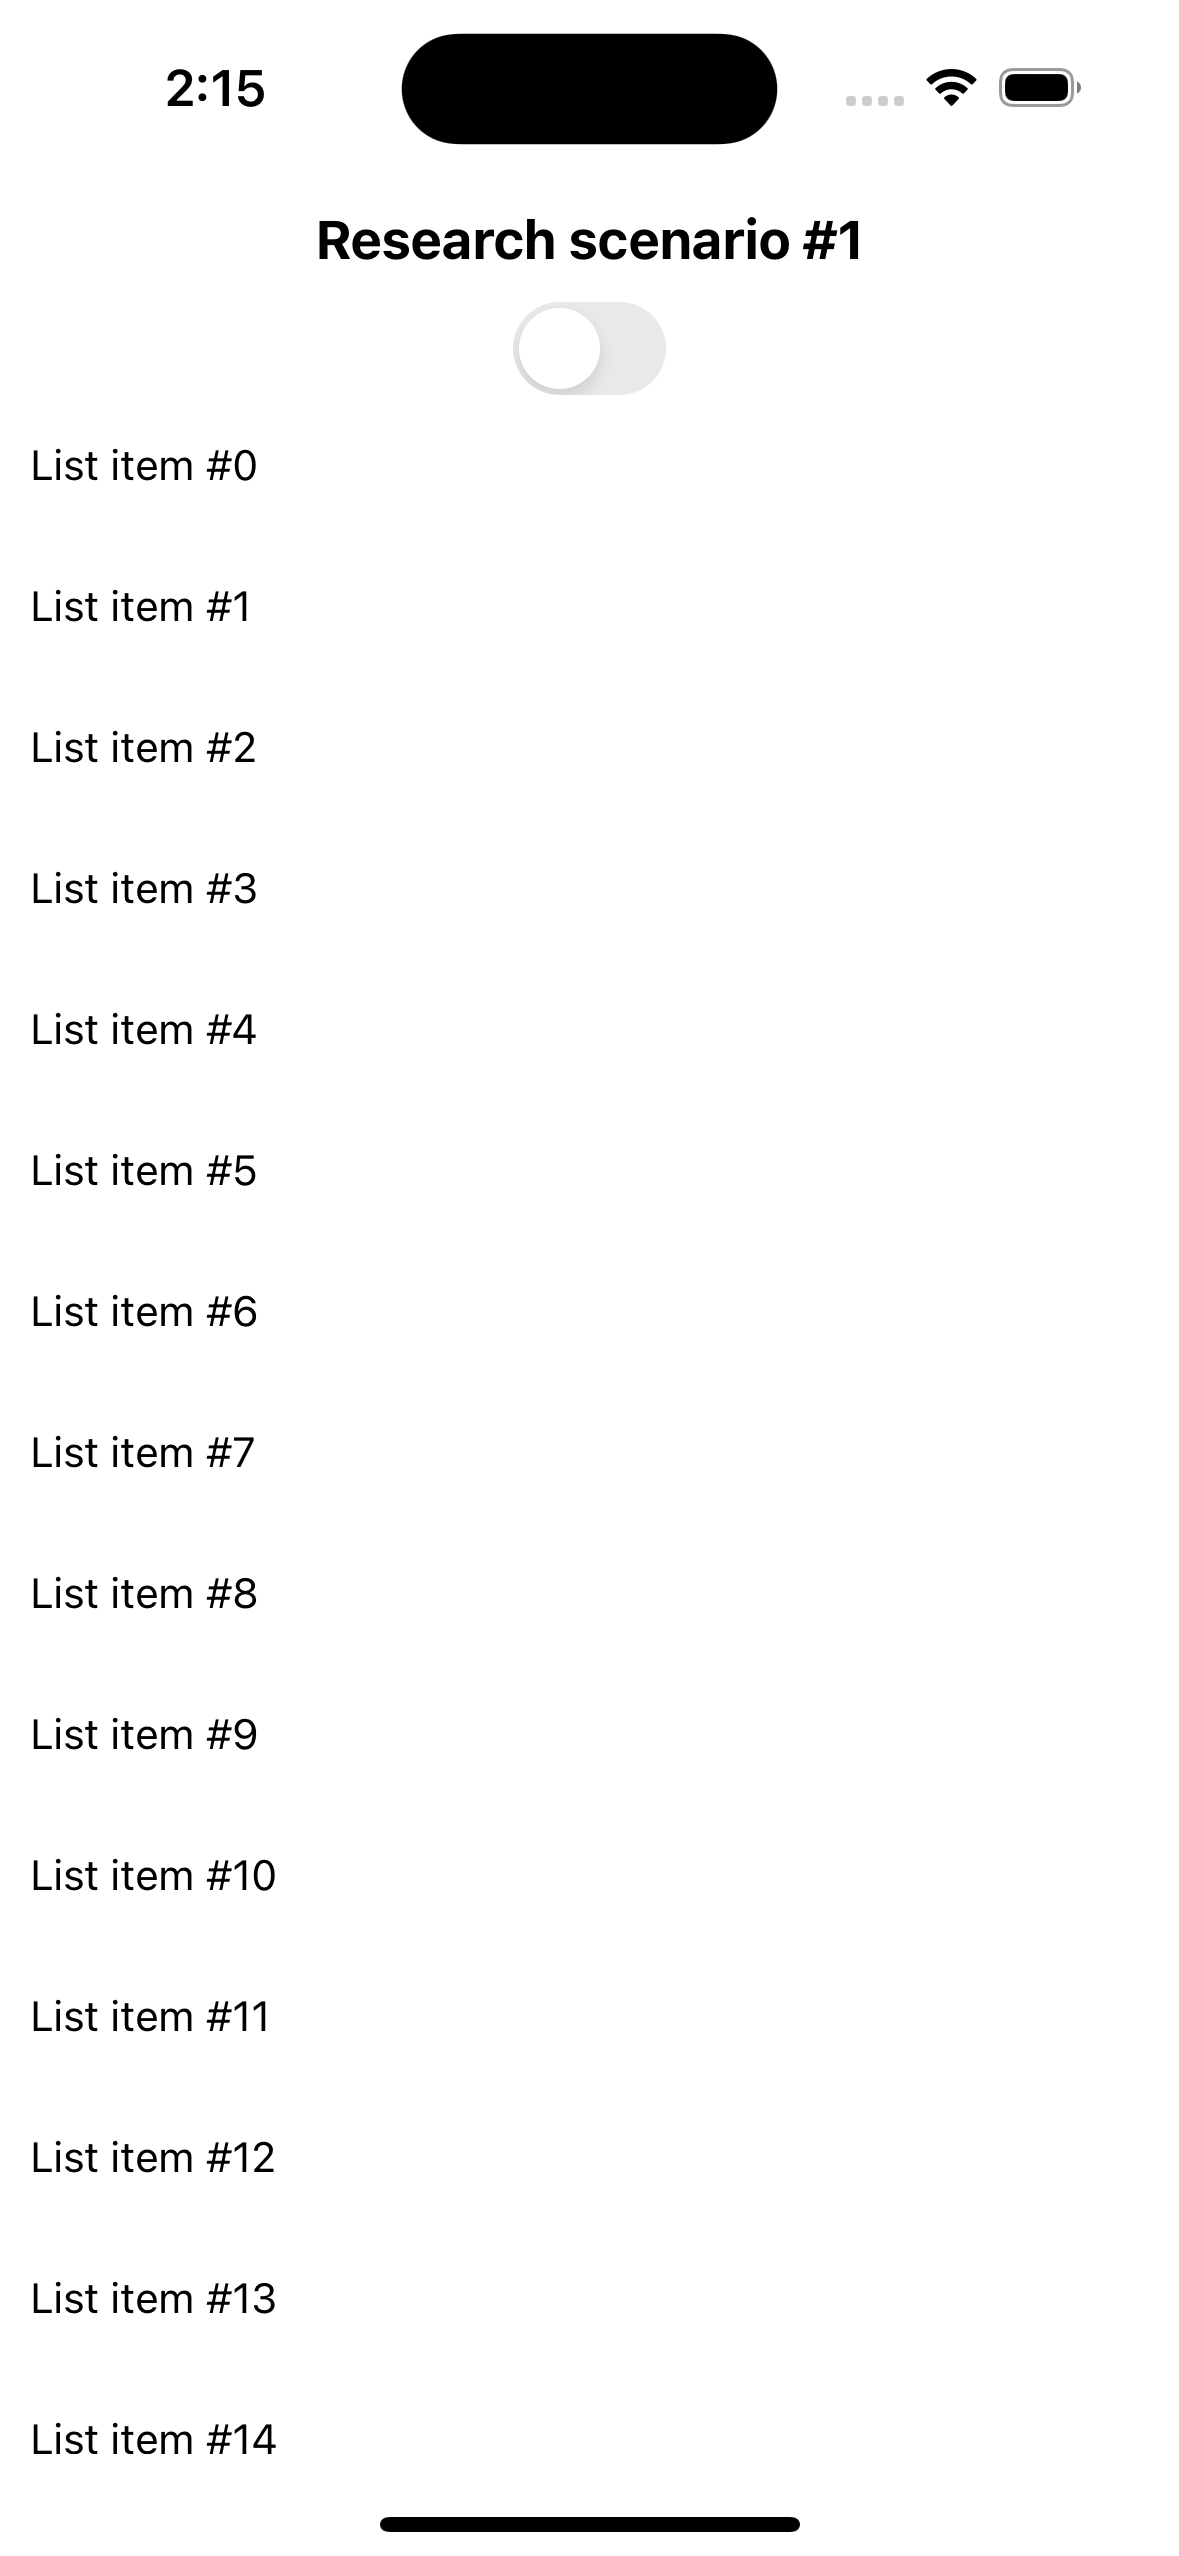
\includegraphics[height=50mm]{img/app1_rn_ios}
    \caption{App 1: React Native iOS (Source: Own work)}
    \label{fig:app1_rn_ios}
  \end{minipage}
\end{figure}

\section{Research scenario 2: Animations}

The application consists of rows of \emph{RotatingIcons} and \emph{GrowingIcons}. The former animates its rotation and the latter animates its size, with different durations and directions.

\begin{figure}[H]
  \begin{minipage}{.47\textwidth}
    \centering
    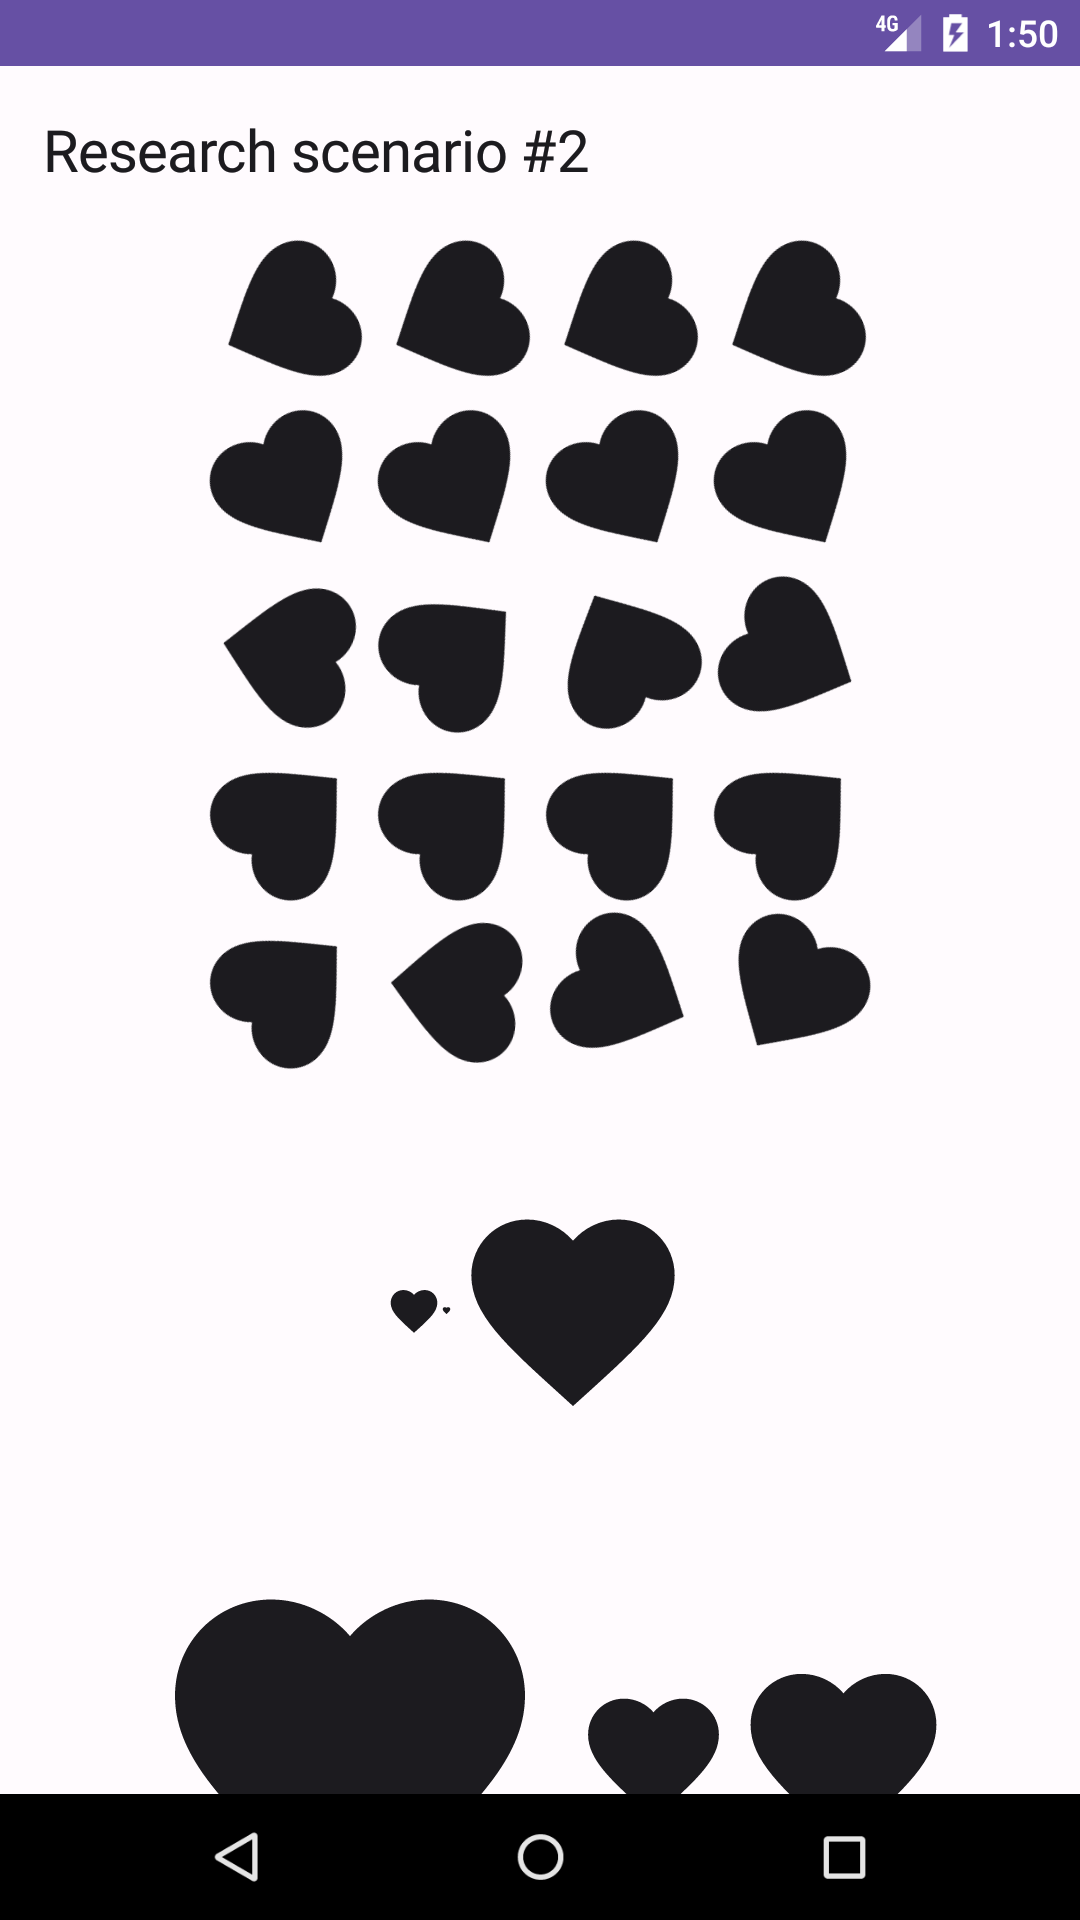
\includegraphics[height=50mm]{img/app2_kotlin}
    \caption{App 2: Kotlin (Source: Own work)}
    \label{fig:app2_kotlin}
  \end{minipage}
  \hfill
  \begin{minipage}{.47\textwidth}
    \centering
    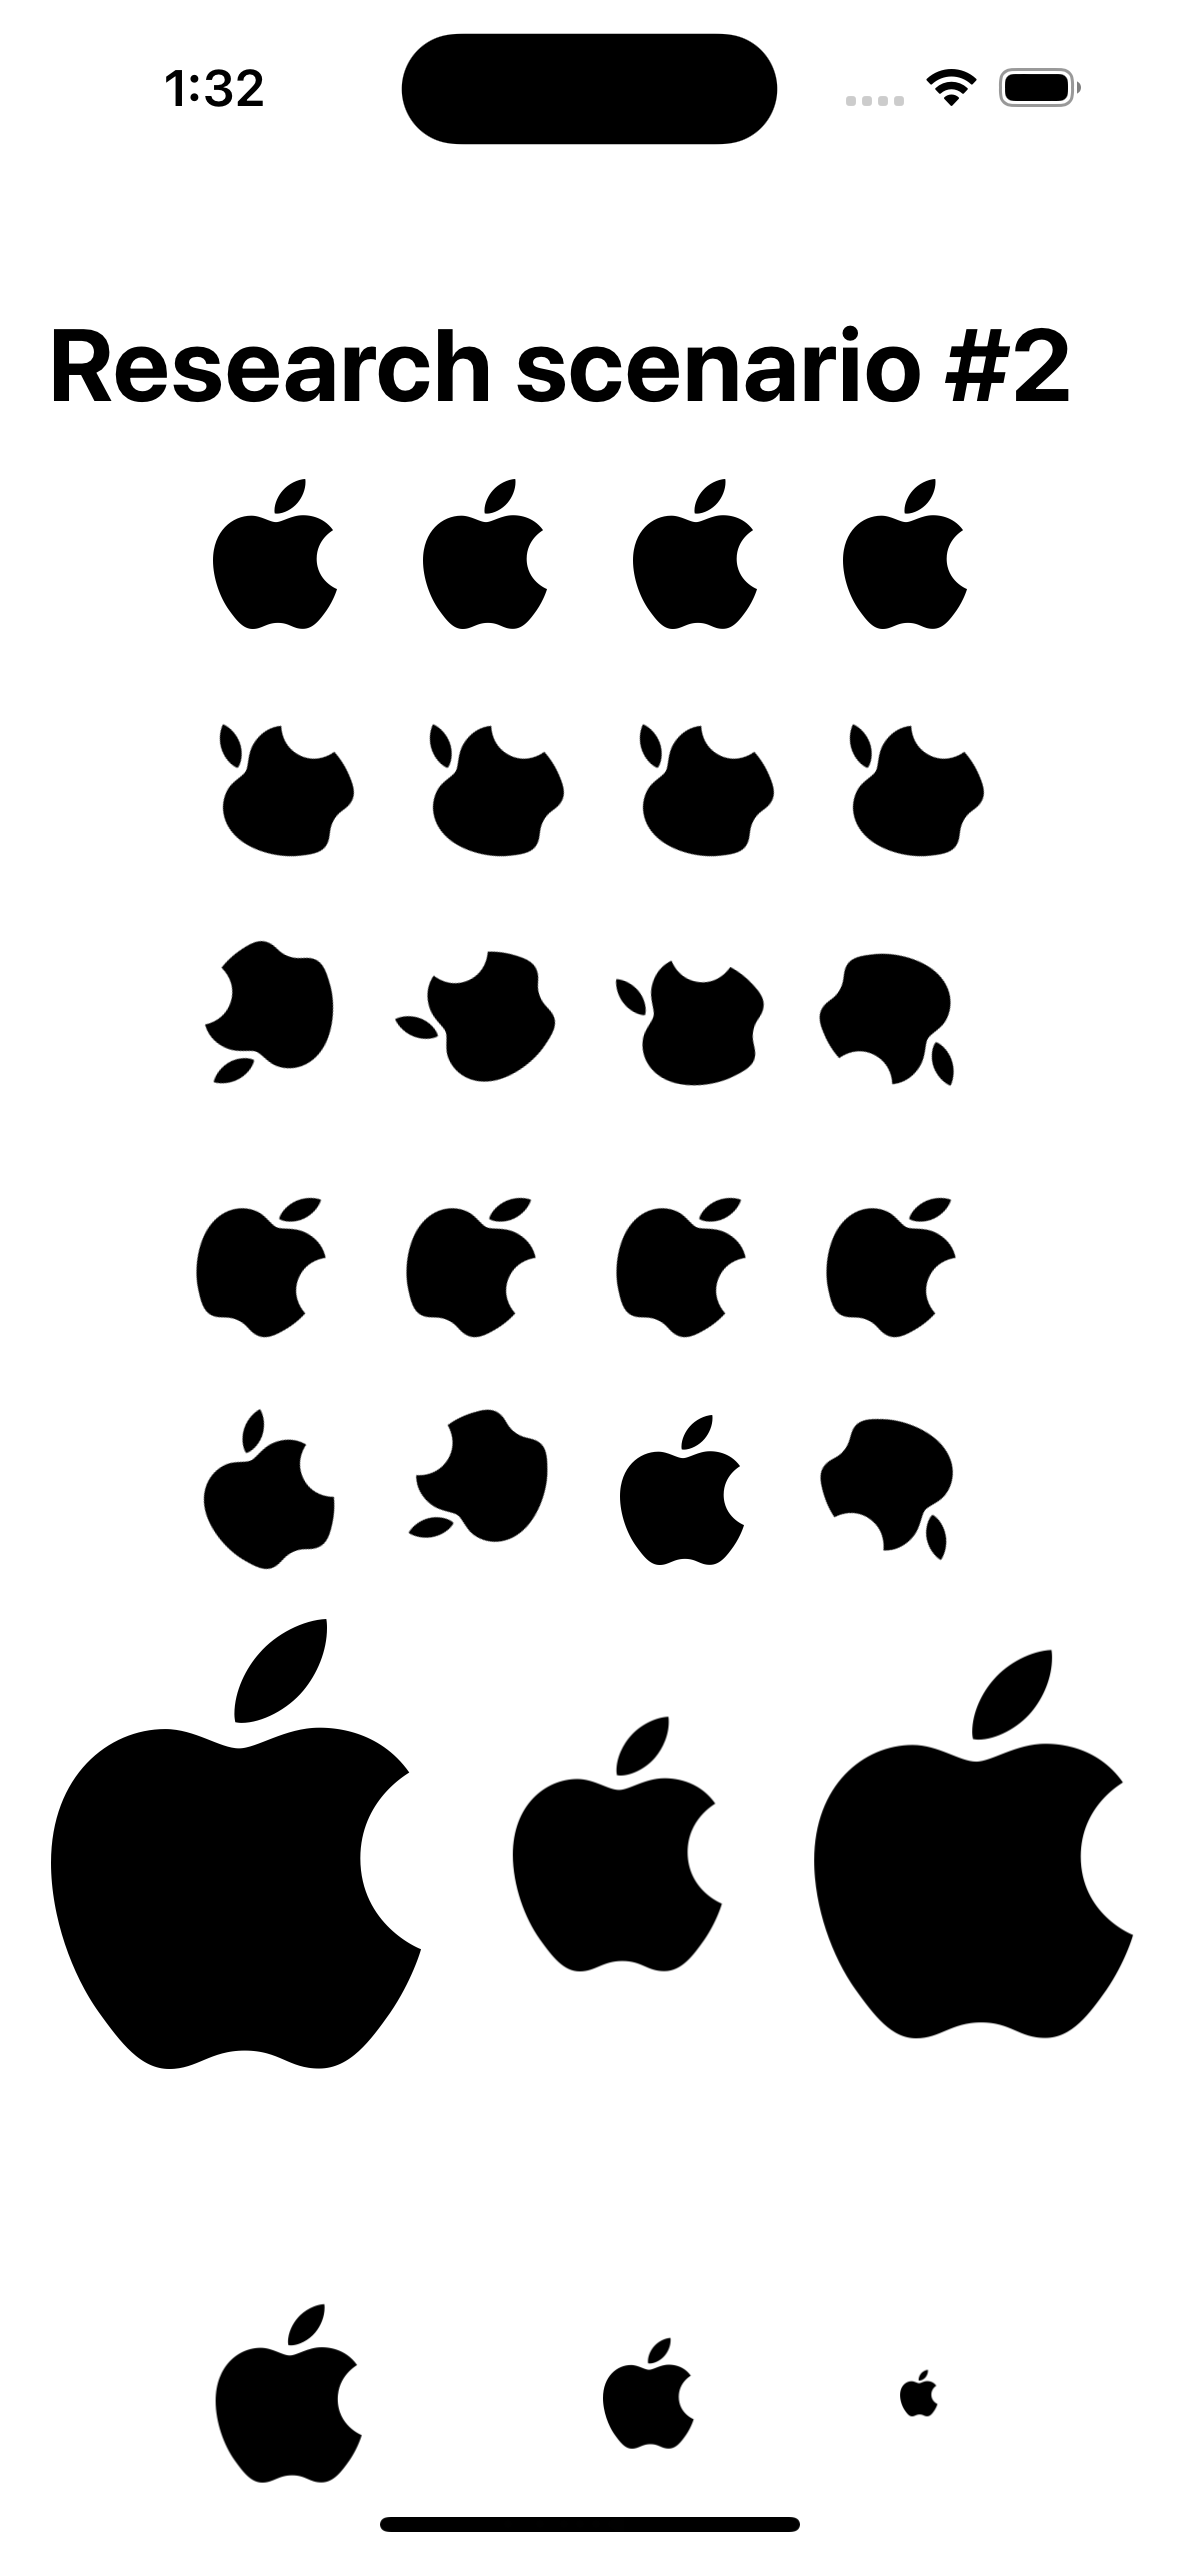
\includegraphics[height=50mm]{img/app2_swift}
    \caption{App 2: Swift (Source: Own work)}
    \label{fig:app2_swift}
  \end{minipage}
\end{figure}

\begin{figure}[H]
\begin{minipage}{.47\textwidth}
  \centering
  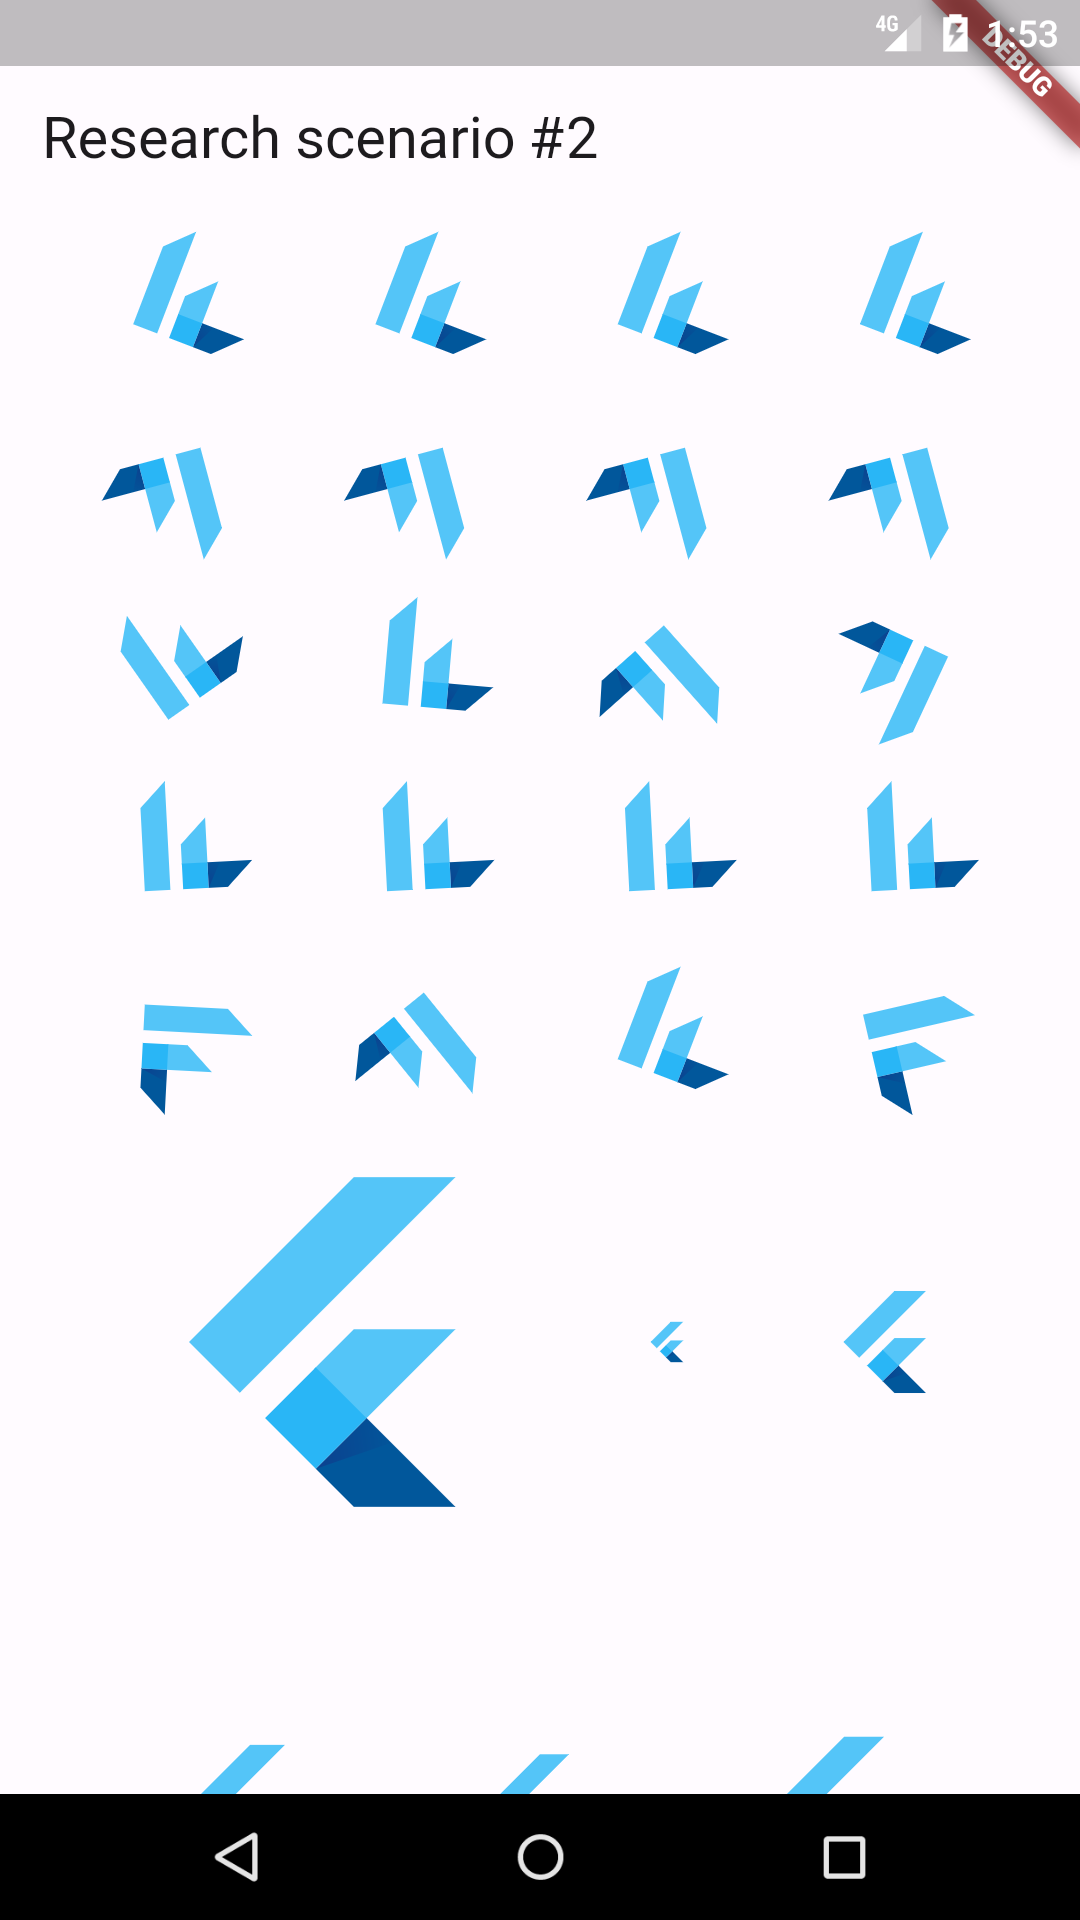
\includegraphics[height=50mm]{img/app2_flutter_android}
  \caption{App 2: Flutter Android (Source: Own work)}
  \label{fig:app2_flutter_android}
\end{minipage}
\hfill
\begin{minipage}{.47\textwidth}
  \centering
  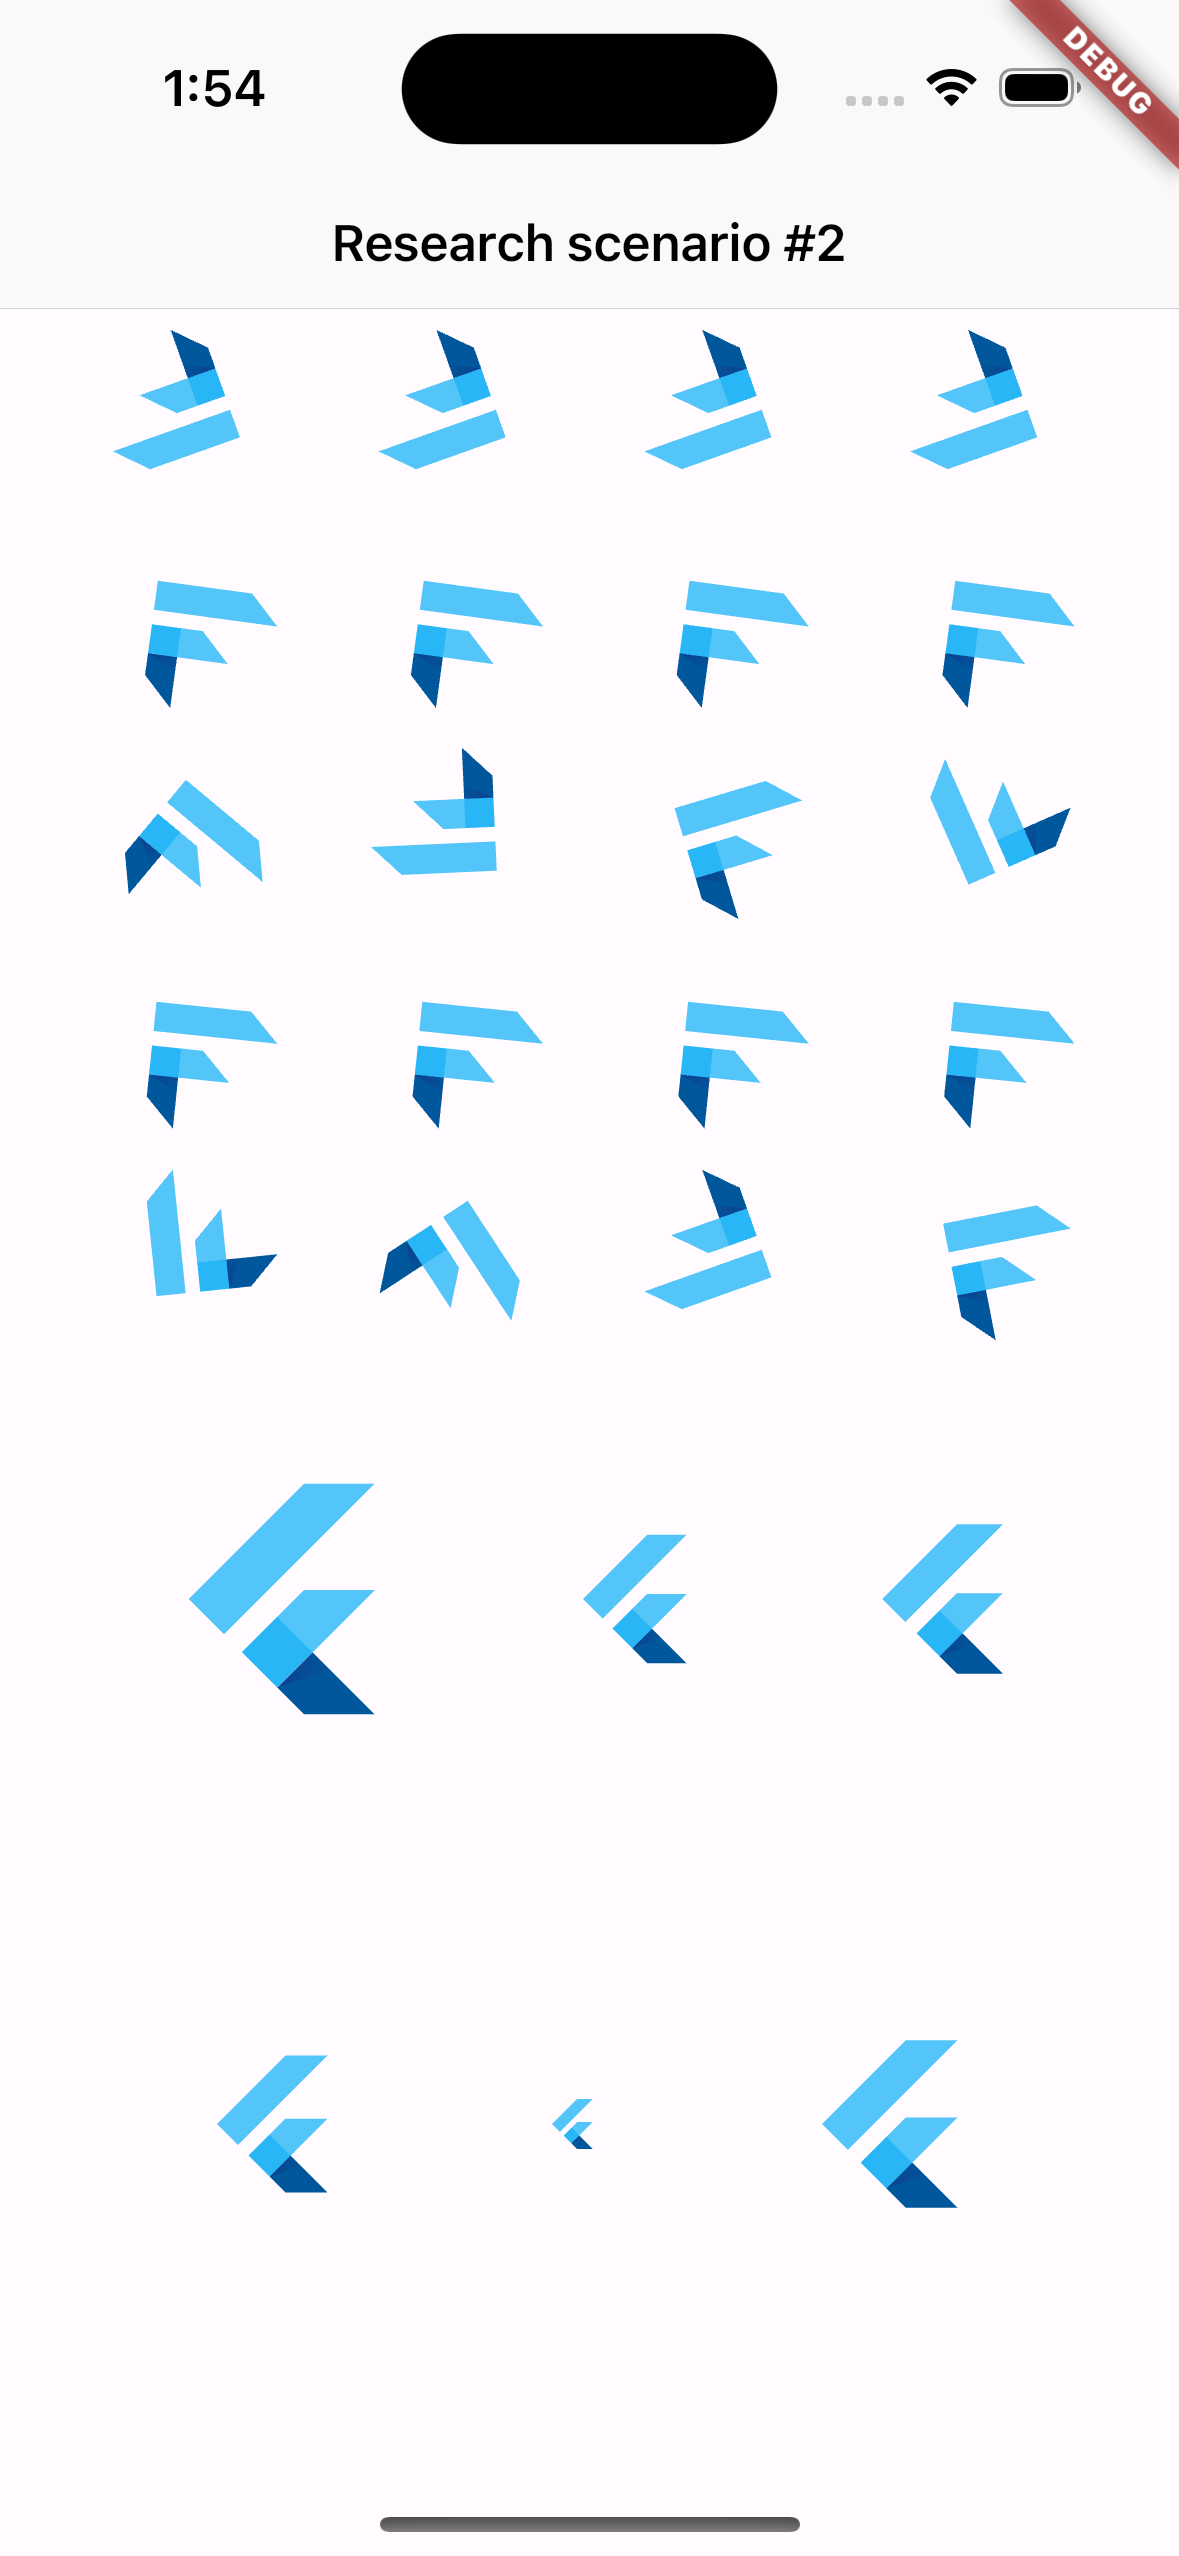
\includegraphics[height=50mm]{img/app2_flutter_ios}
  \caption{App 2: Flutter iOS (Source: Own work)}
  \label{fig:app2_flutter_ios}
\end{minipage}
\end{figure}

\begin{figure}[H]
\begin{minipage}{.47\textwidth}
  \centering
  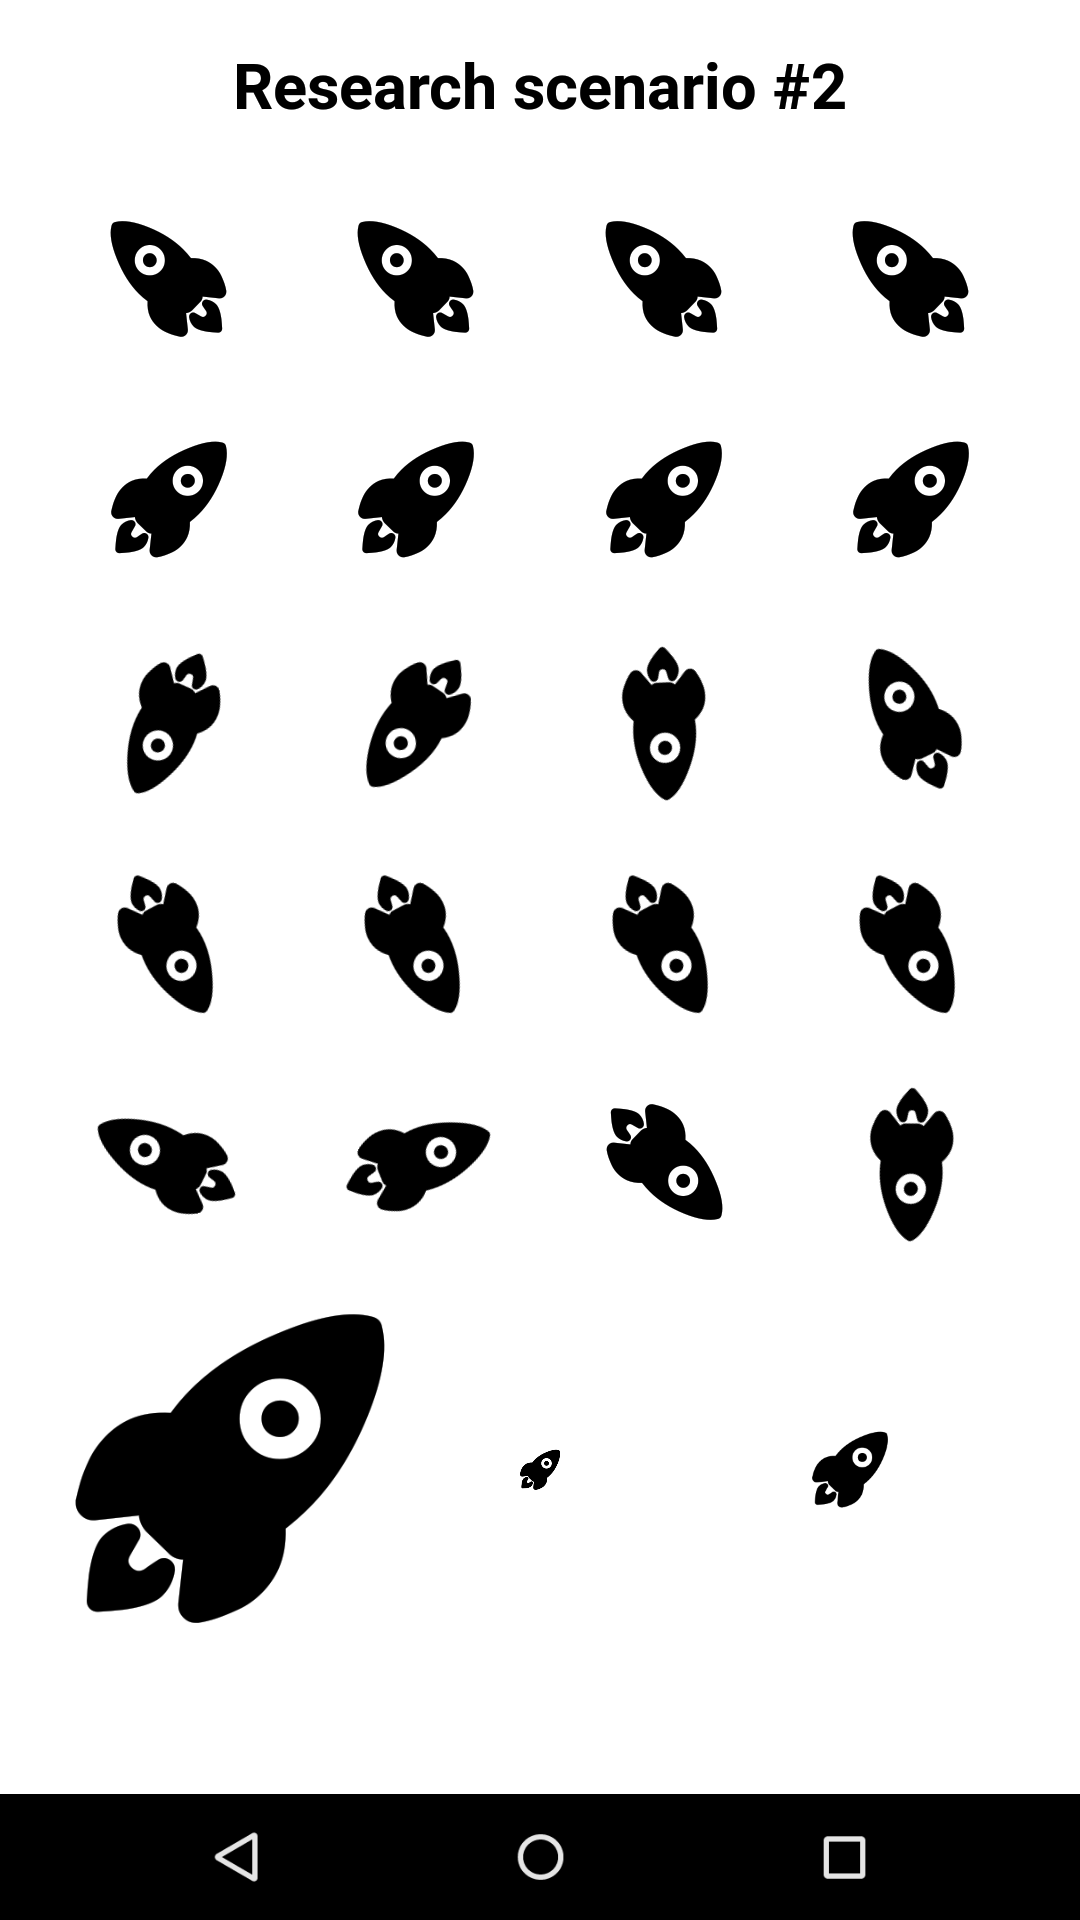
\includegraphics[height=50mm]{img/app2_rn_android}
  \caption{App 1: React Native Android (Source: Own work)}
  \label{fig:app2_rn_android}
\end{minipage}
\hfill
\begin{minipage}{.47\textwidth}
  \centering
  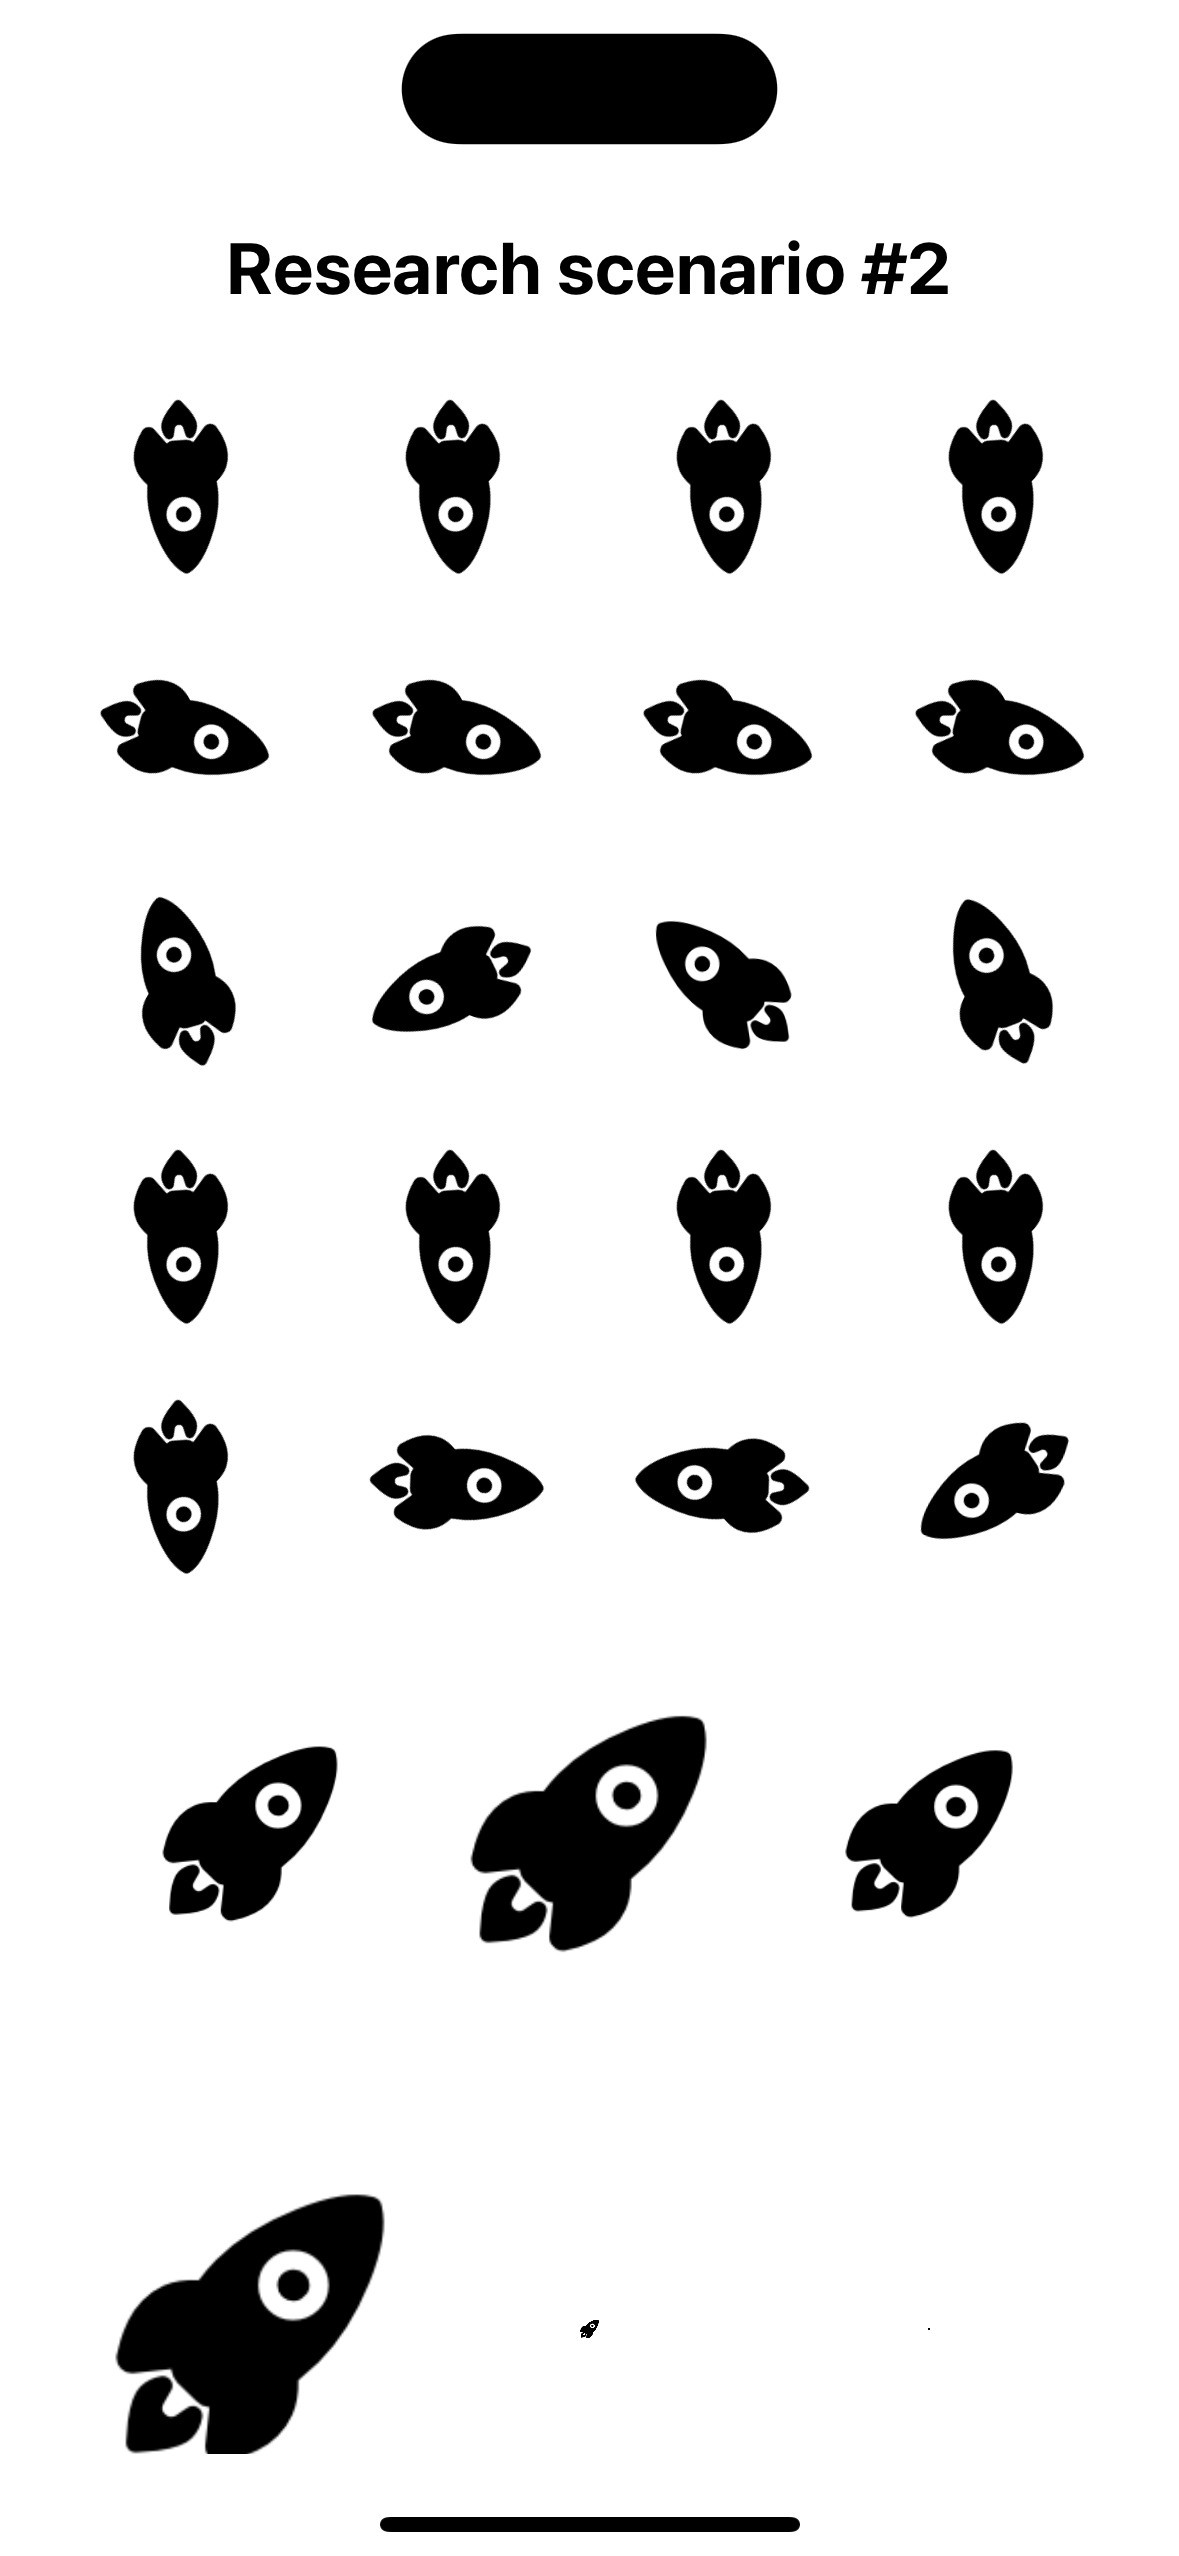
\includegraphics[height=50mm]{img/app2_rn_ios}
  \caption{App 1: React Native iOS (Source: Own work)}
  \label{fig:app2_rn_ios}
\end{minipage}
\end{figure}

\section{Research scenario 3: File I/O}

The application consists of two \emph{Buttons} and a \emph{Grid View}. The first \emph{Button} saves a text file on the device and the second allows selecting images from the Gallery. Selected images are then presented in a 2-column scrollable \emph{Grid view}.

\begin{figure}[H]
  \begin{minipage}{.47\textwidth}
    \centering
    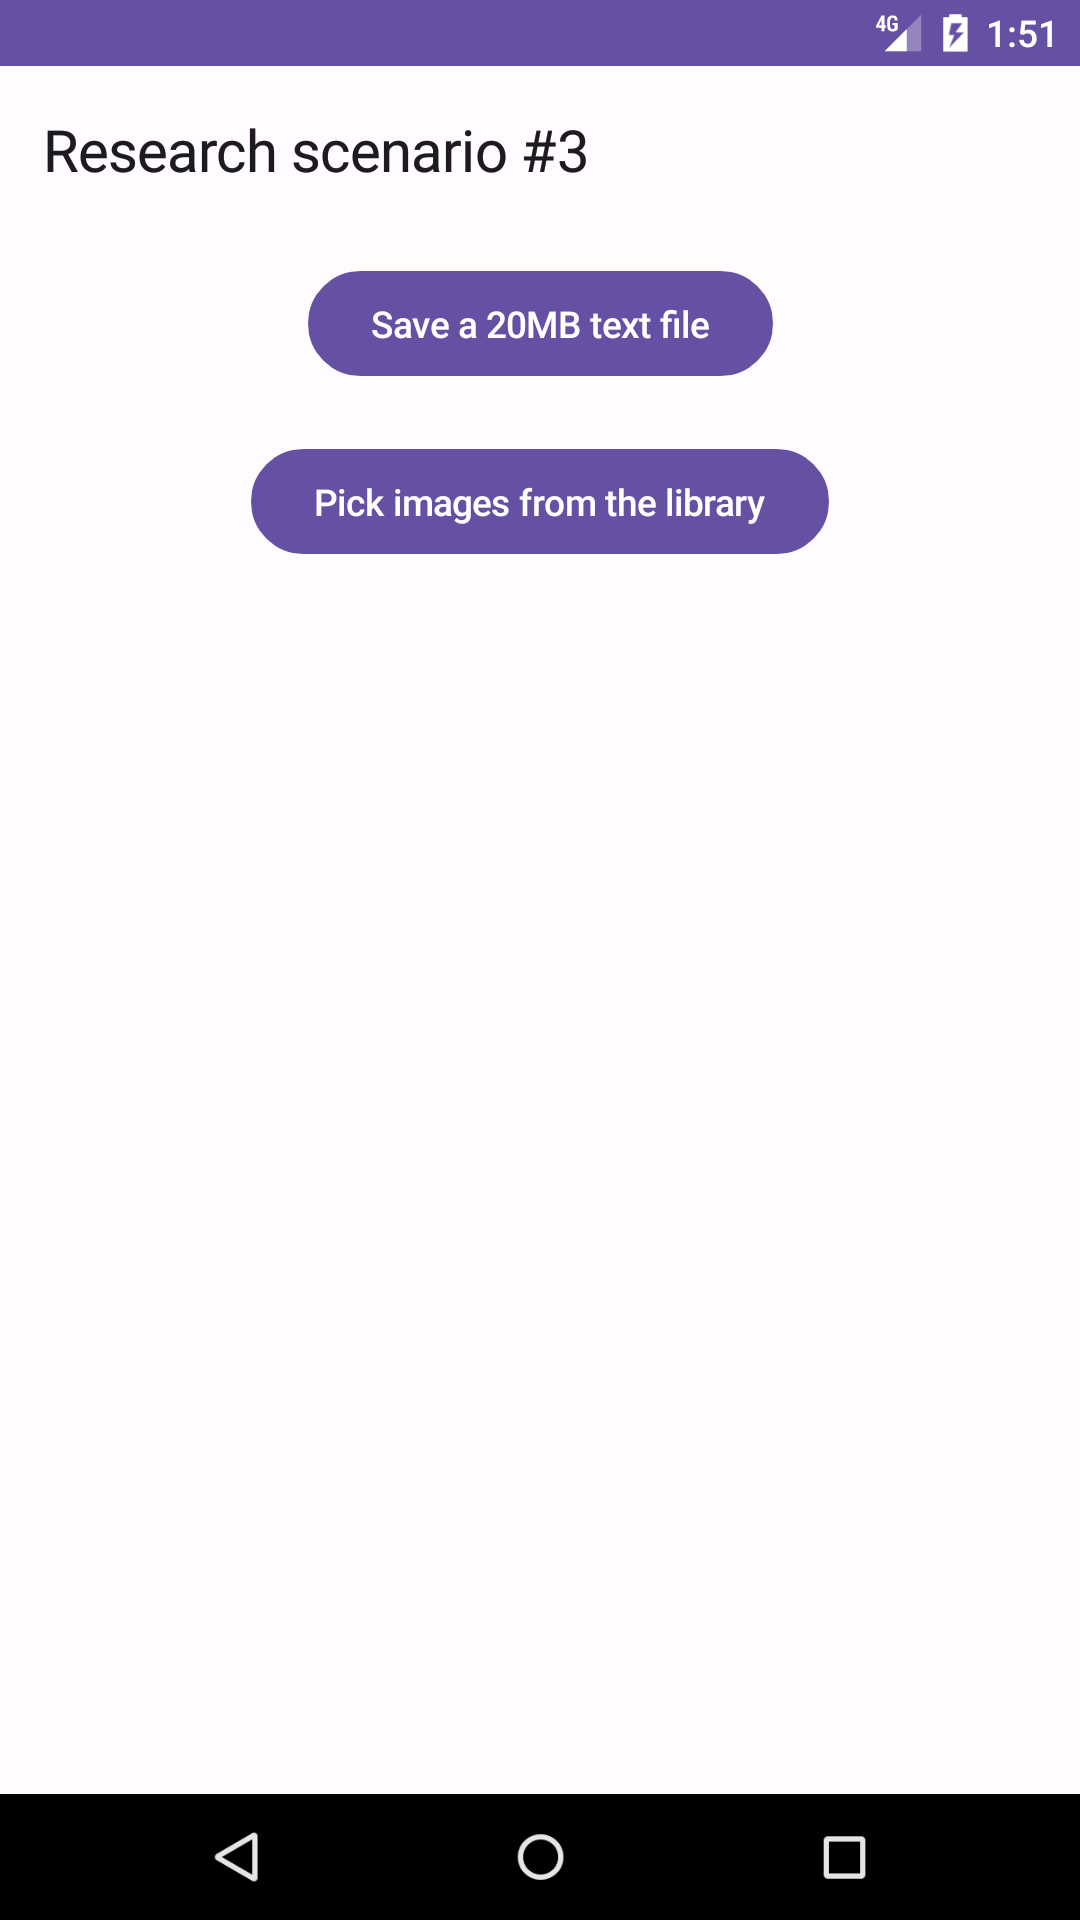
\includegraphics[height=50mm]{img/app3_kotlin}
    \caption{App 3: Kotlin (Source: Own work)}
    \label{fig:app3_kotlin}
  \end{minipage}
  \hfill
  \begin{minipage}{.47\textwidth}
    \centering
    \frame{
      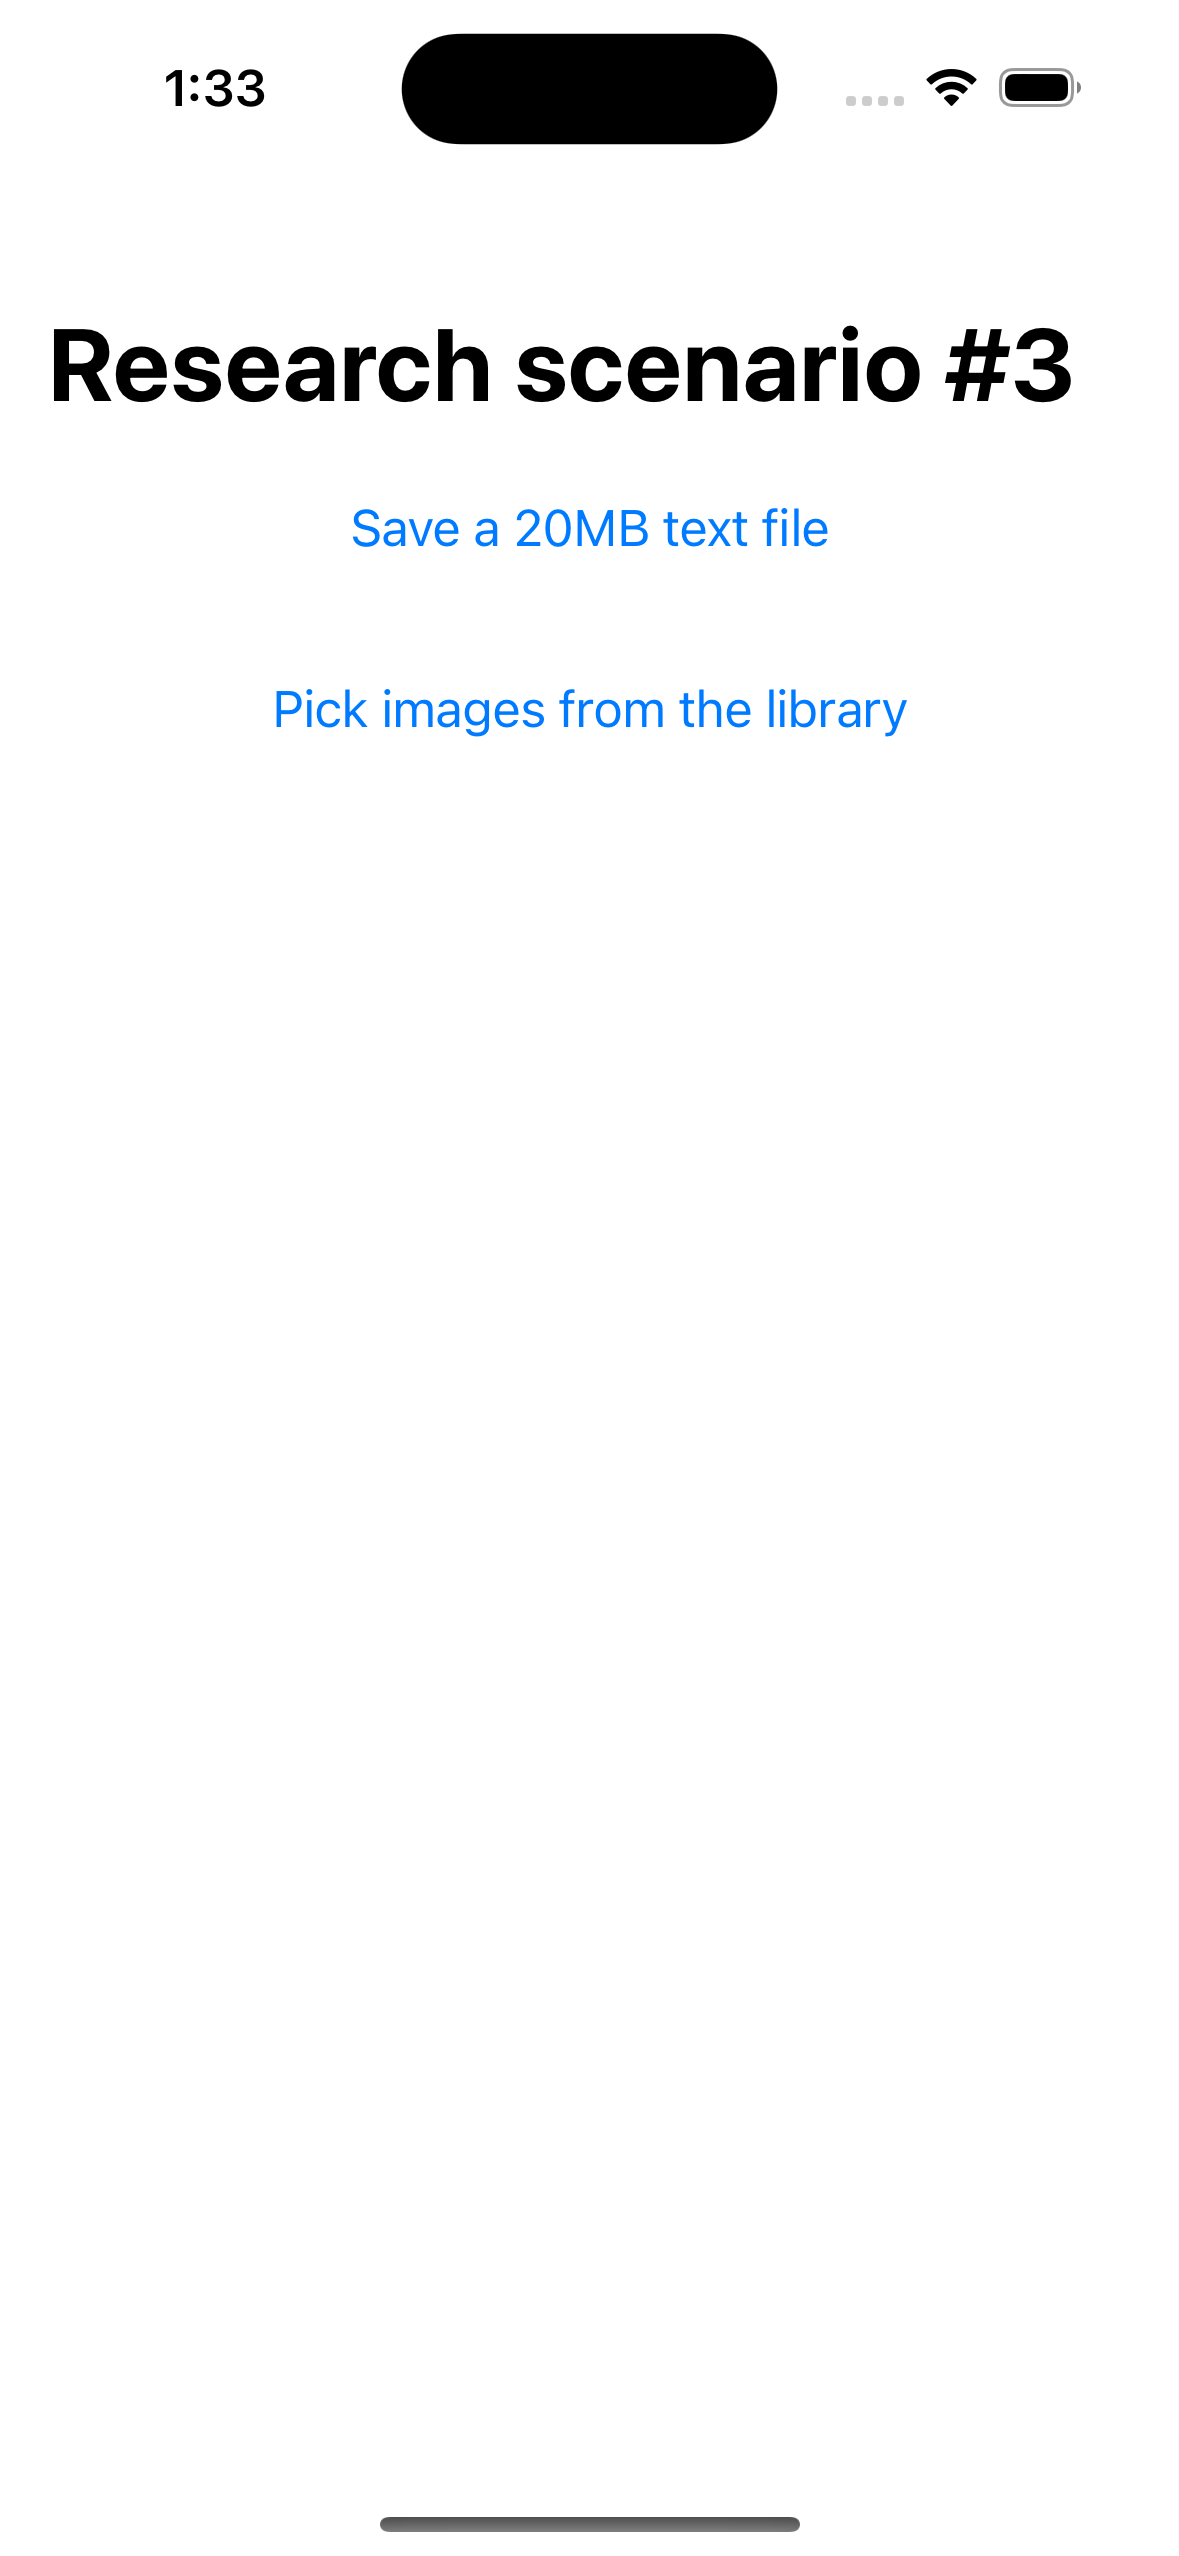
\includegraphics[height=50mm]{img/app3_swift}
    }
    \caption{App 3: Swift (Source: Own work)}
    \label{fig:app3_swift}
  \end{minipage}
\end{figure}

\begin{figure}[H]
\begin{minipage}{.47\textwidth}
  \centering
  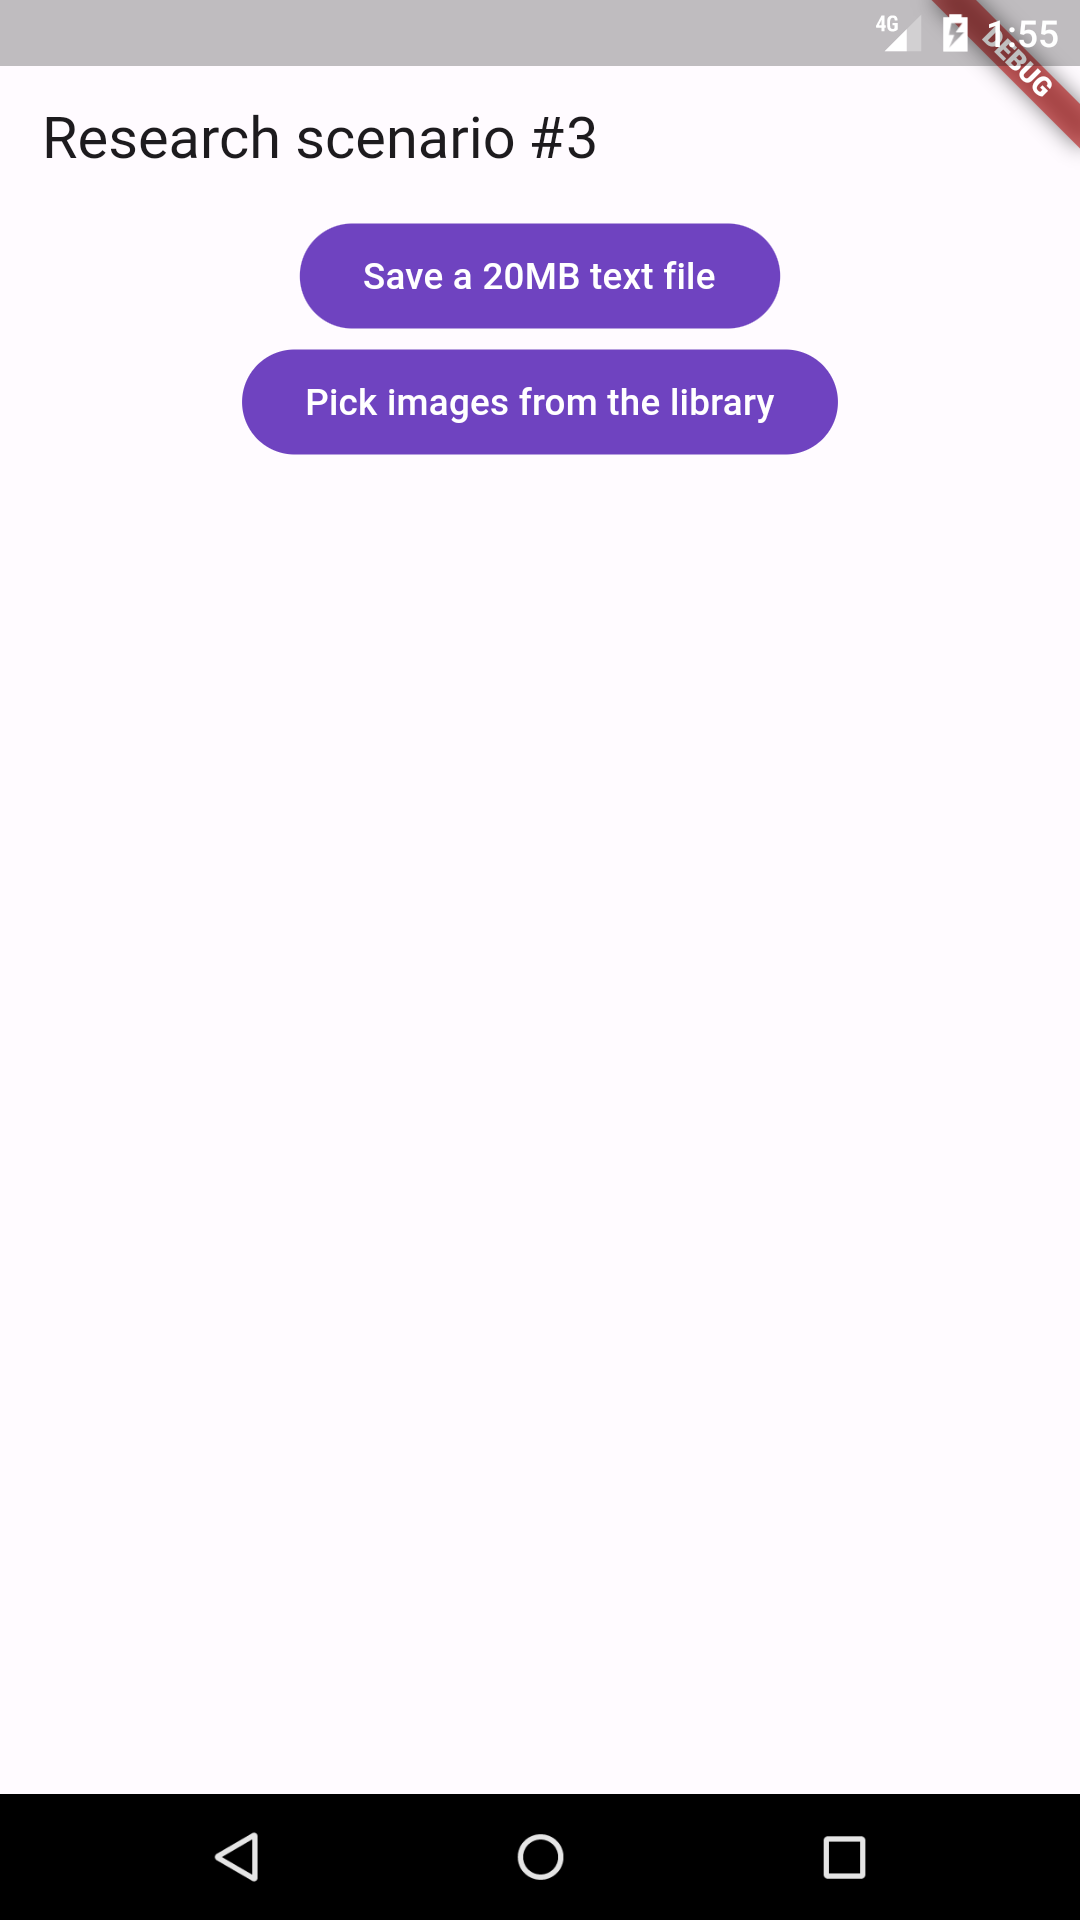
\includegraphics[height=50mm]{img/app3_flutter_android}
  \caption{App 3: Flutter Android (Source: Own work)}
  \label{fig:app3_flutter_android}
\end{minipage}
\hfill
\begin{minipage}{.47\textwidth}
  \centering
  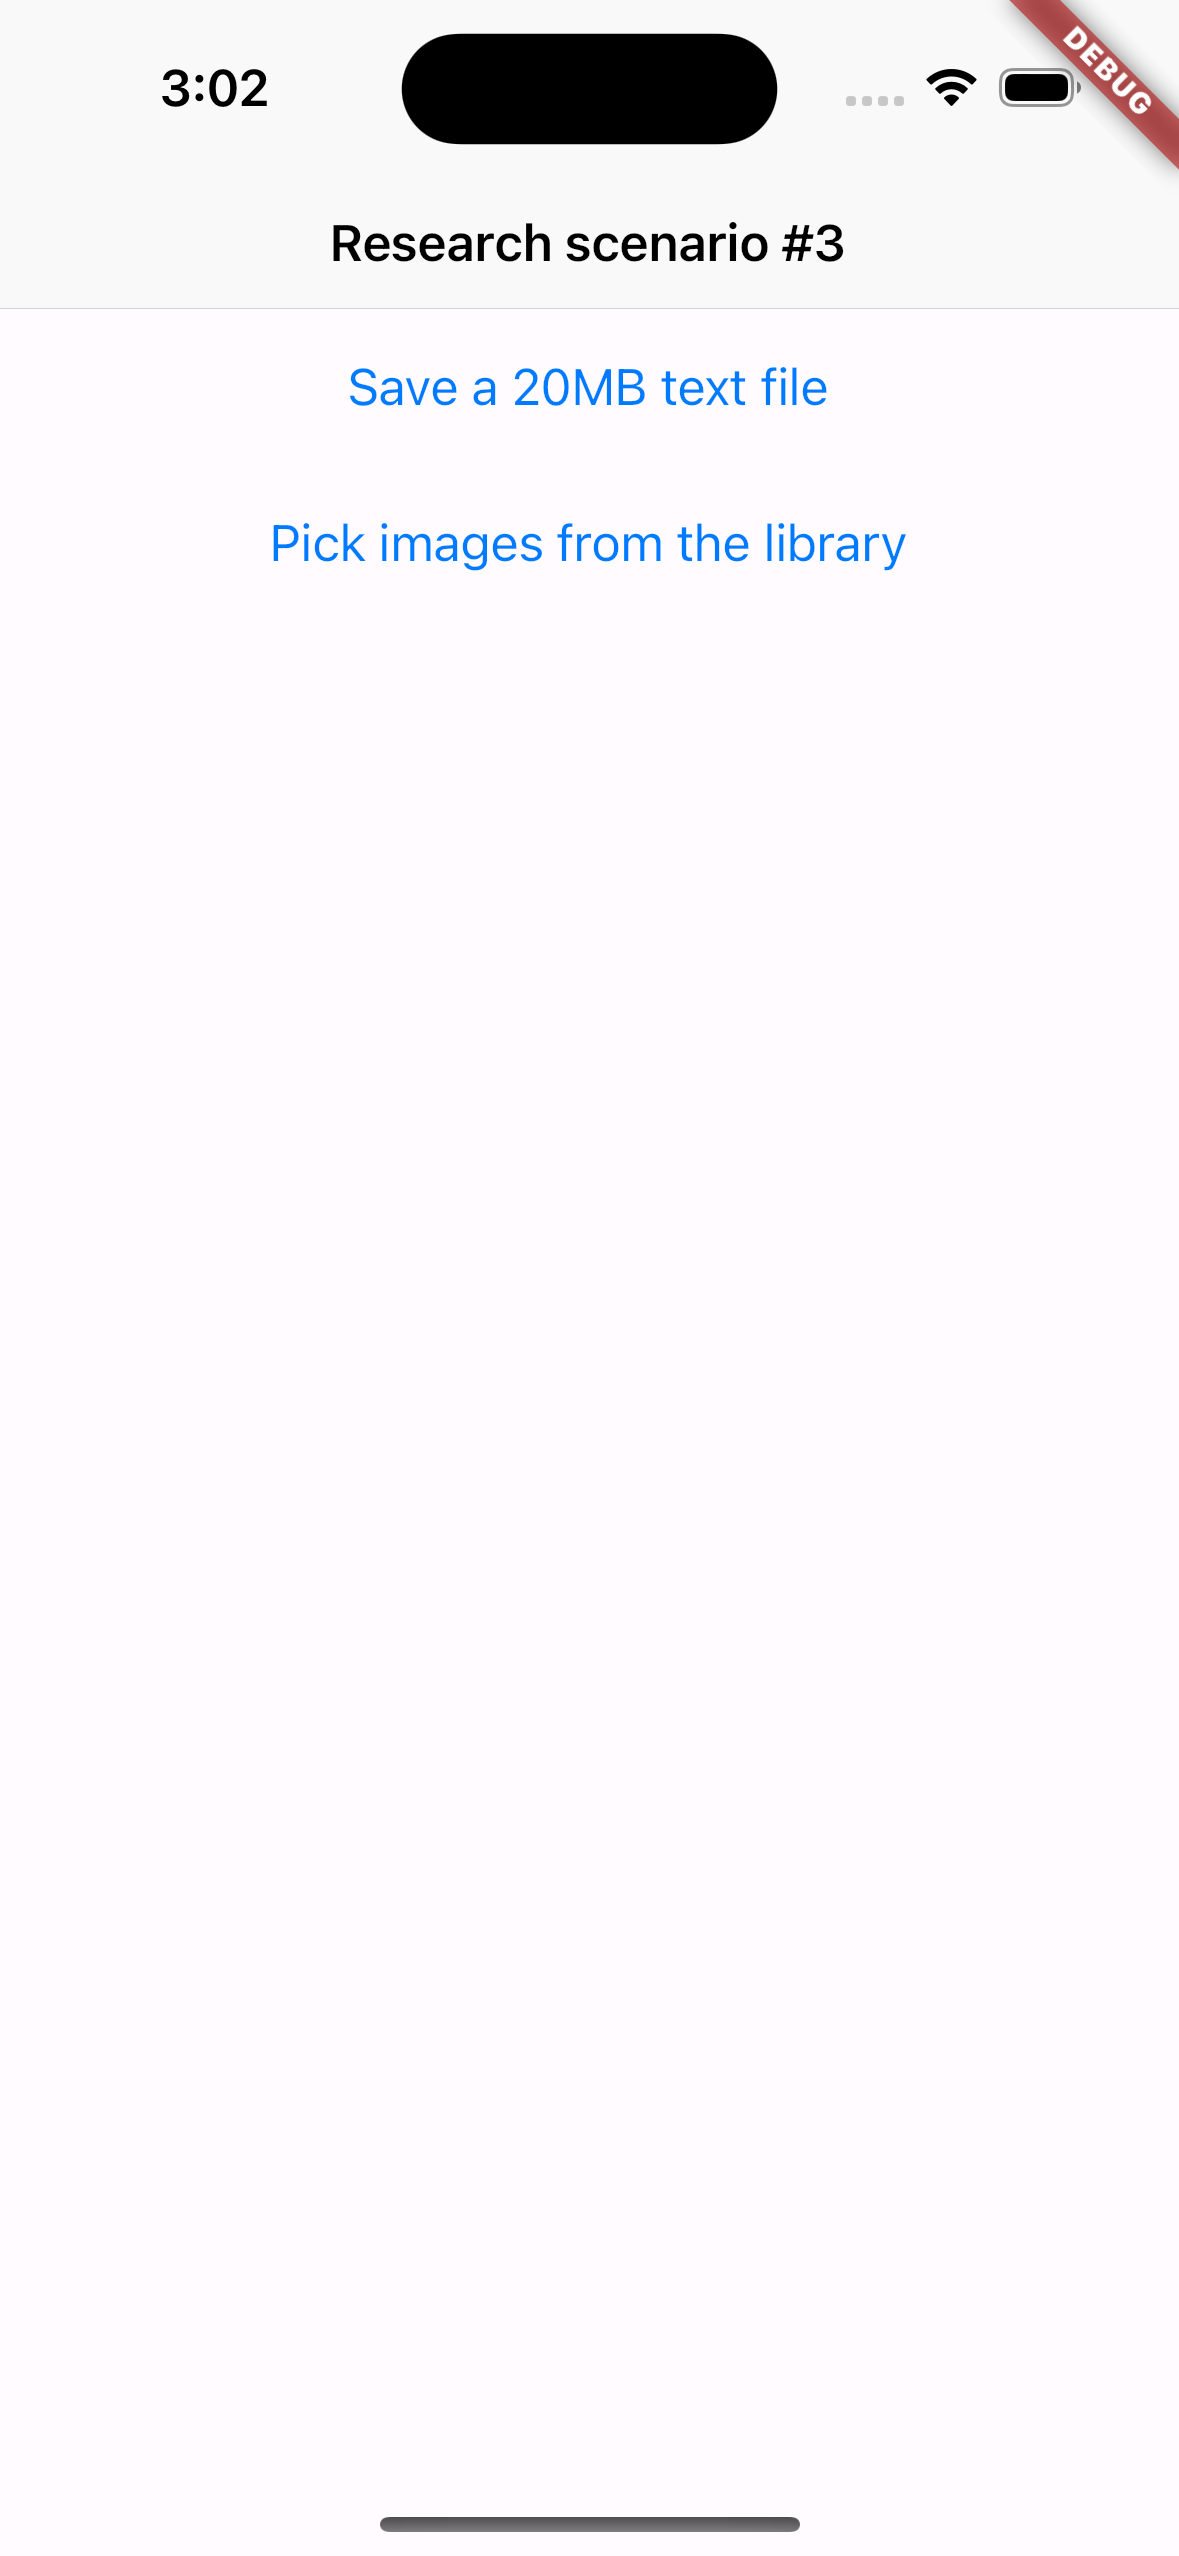
\includegraphics[height=50mm]{img/app3_flutter_ios}
  \caption{App 3: Flutter iOS (Source: Own work)}
  \label{fig:app3_flutter_ios}
\end{minipage}
\end{figure}

\begin{figure}[H]
\begin{minipage}{.47\textwidth}
  \centering
  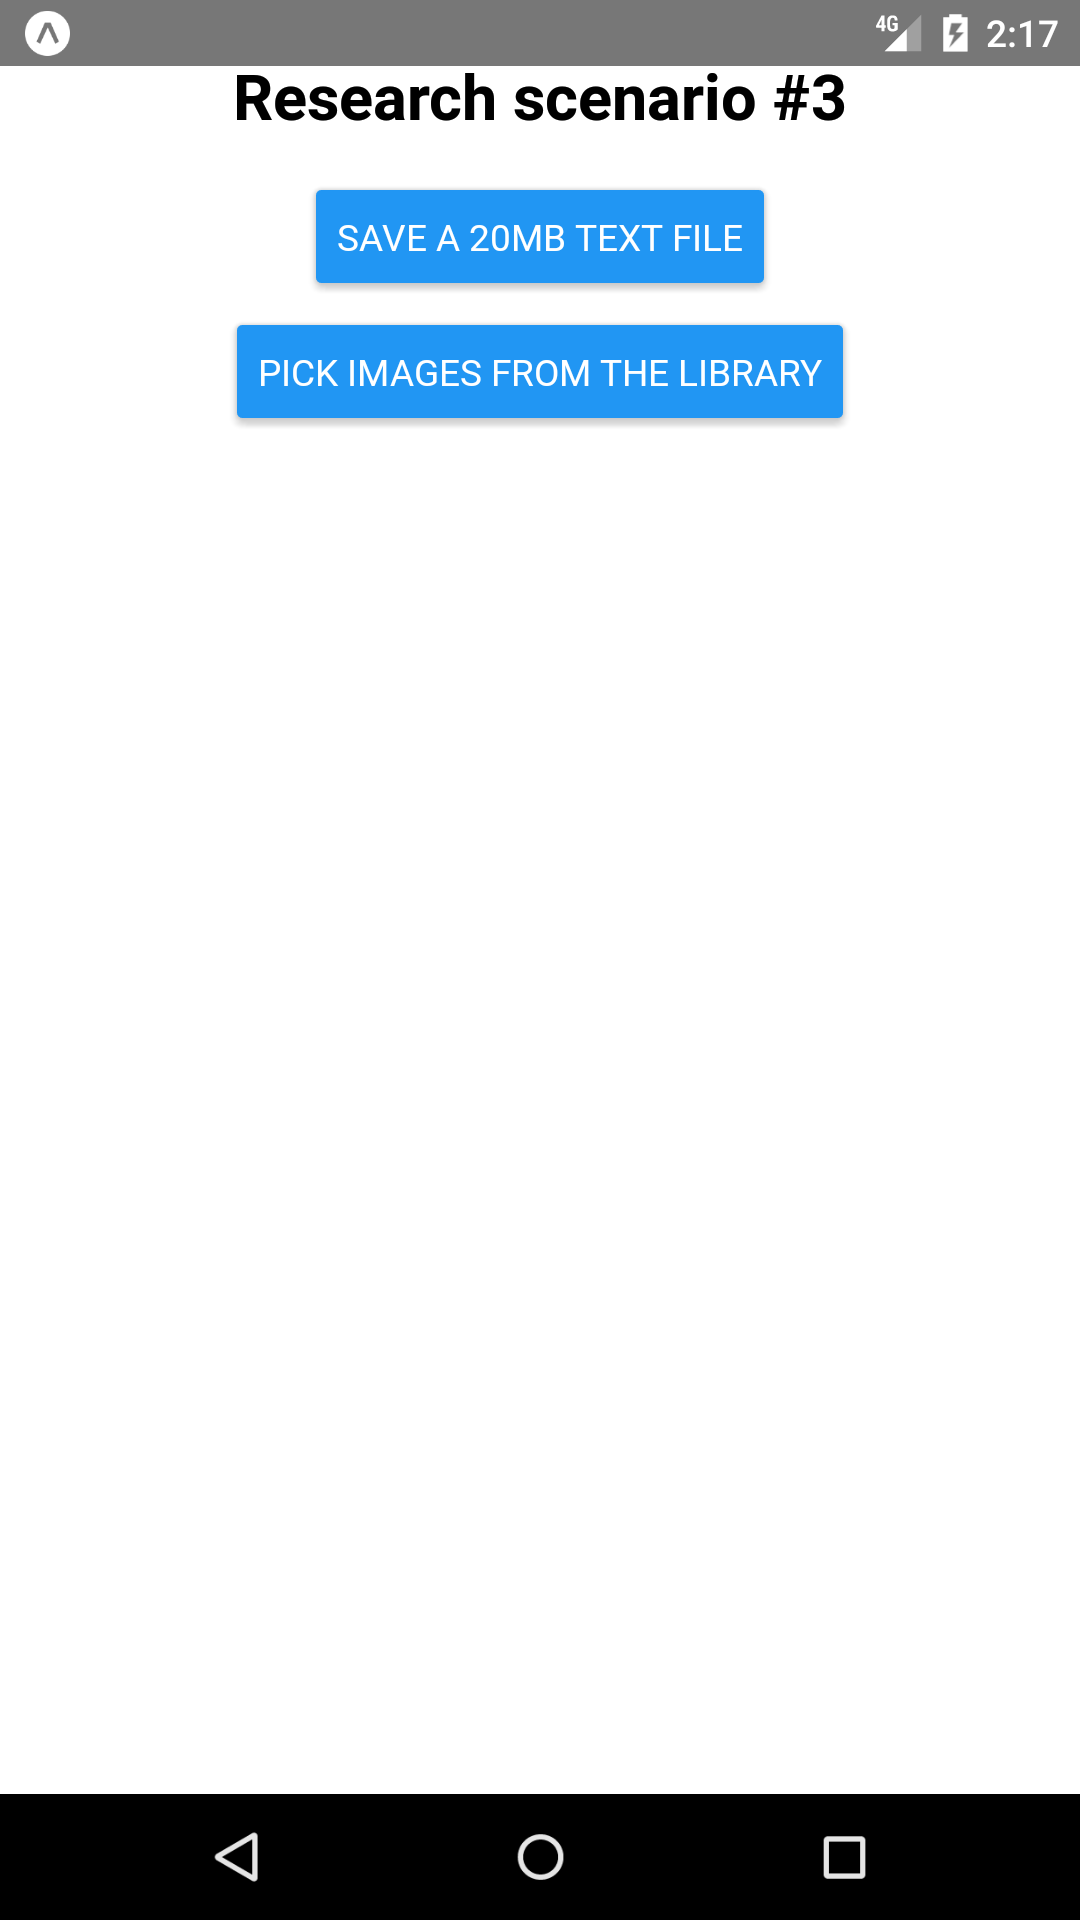
\includegraphics[height=50mm]{img/app3_rn_android}
  \caption{App 3: React Native Android (Source: Own work)}
  \label{fig:app3_rn_android}
\end{minipage}
\hfill
\begin{minipage}{.47\textwidth}
  \centering
  \frame{
    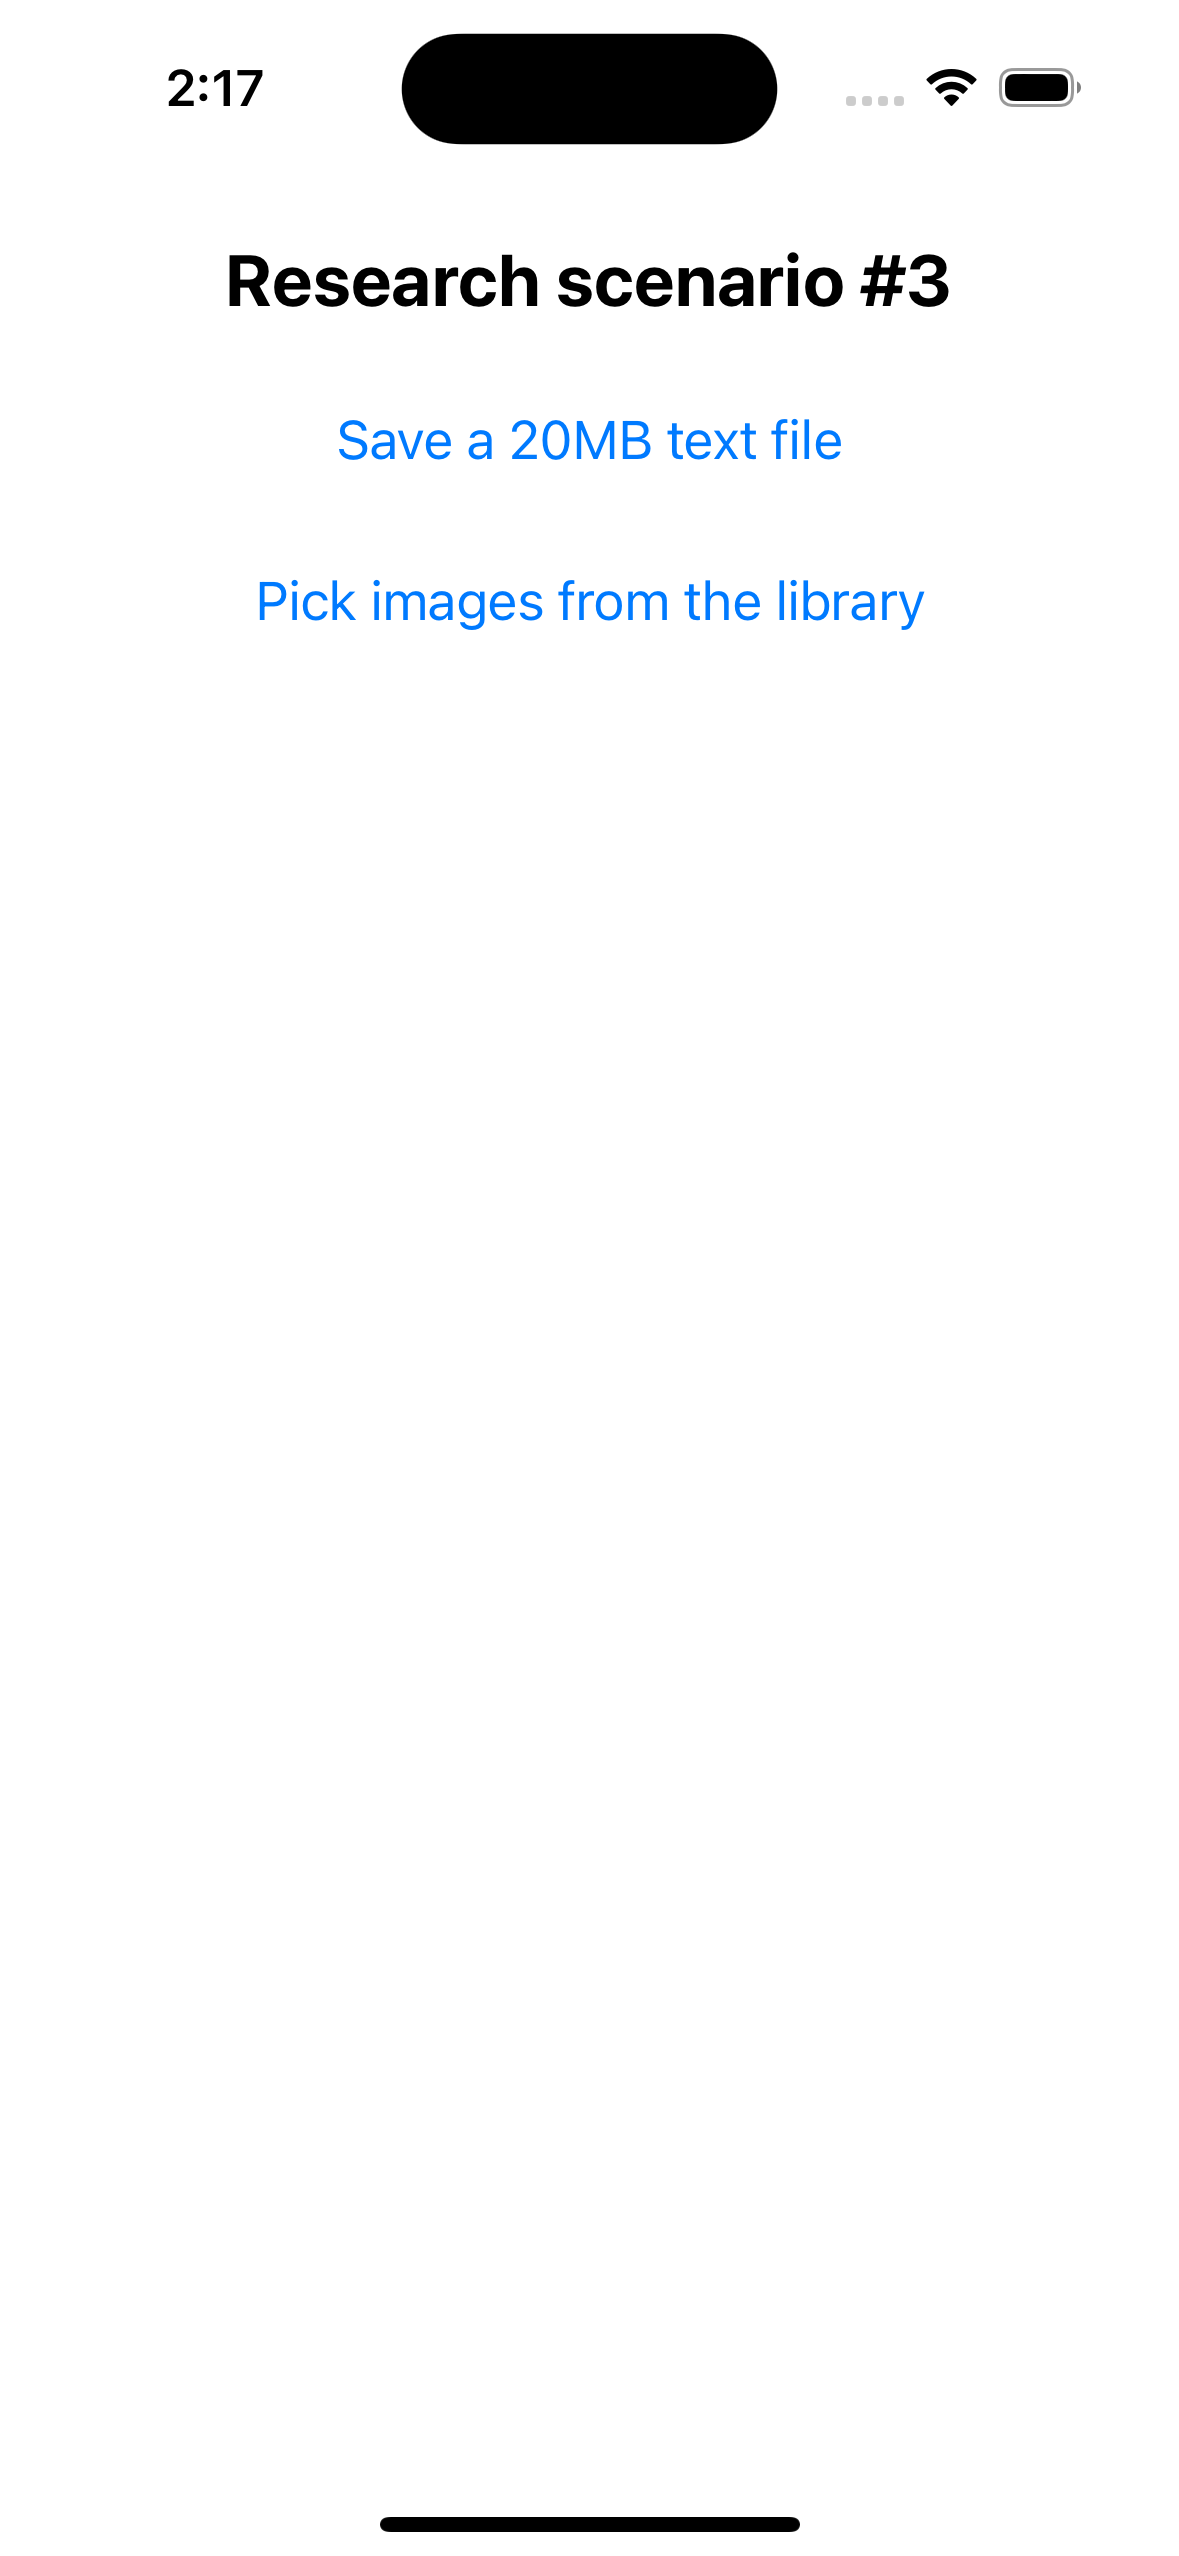
\includegraphics[height=50mm]{img/app3_rn_ios}
  }
  \caption{App 3: React Native iOS (Source: Own work)}
  \label{fig:app3_rn_ios}
\end{minipage}
\end{figure}

\section{Research scenario 4: Common UI elements}

The application consists of three views: \emph{Controls Page}, \emph{Form Page} and \emph{External Page}. Various common UI components are utilized as well as the bottom tab bar navigation.

\begin{figure}[H]
  \begin{minipage}{.31\textwidth}
    \centering
    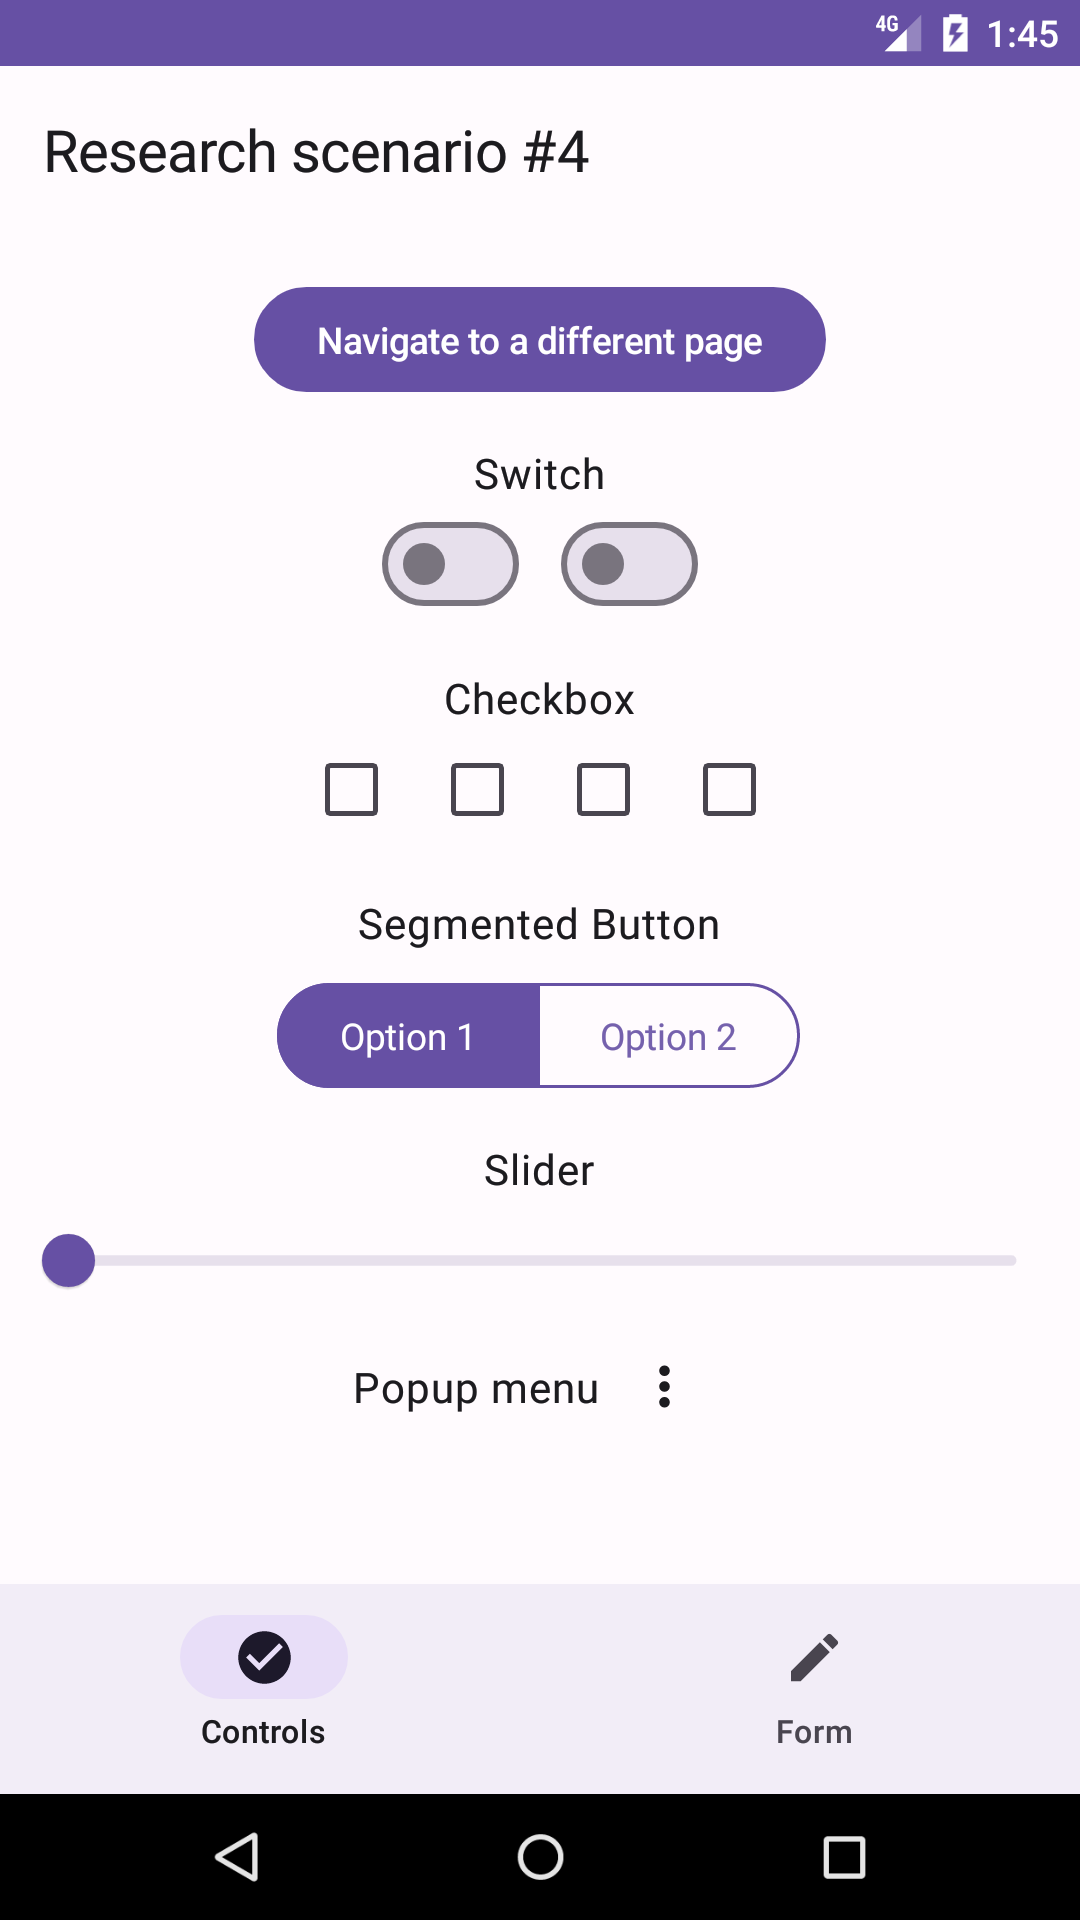
\includegraphics[height=50mm]{img/app4_1_kotlin}
    \caption{App 4 (1/3): Kotlin (Source: Own work)}
    \label{fig:app4_1_kotlin}
  \end{minipage}
  \hfill
  \begin{minipage}{.31\textwidth}
    \centering
    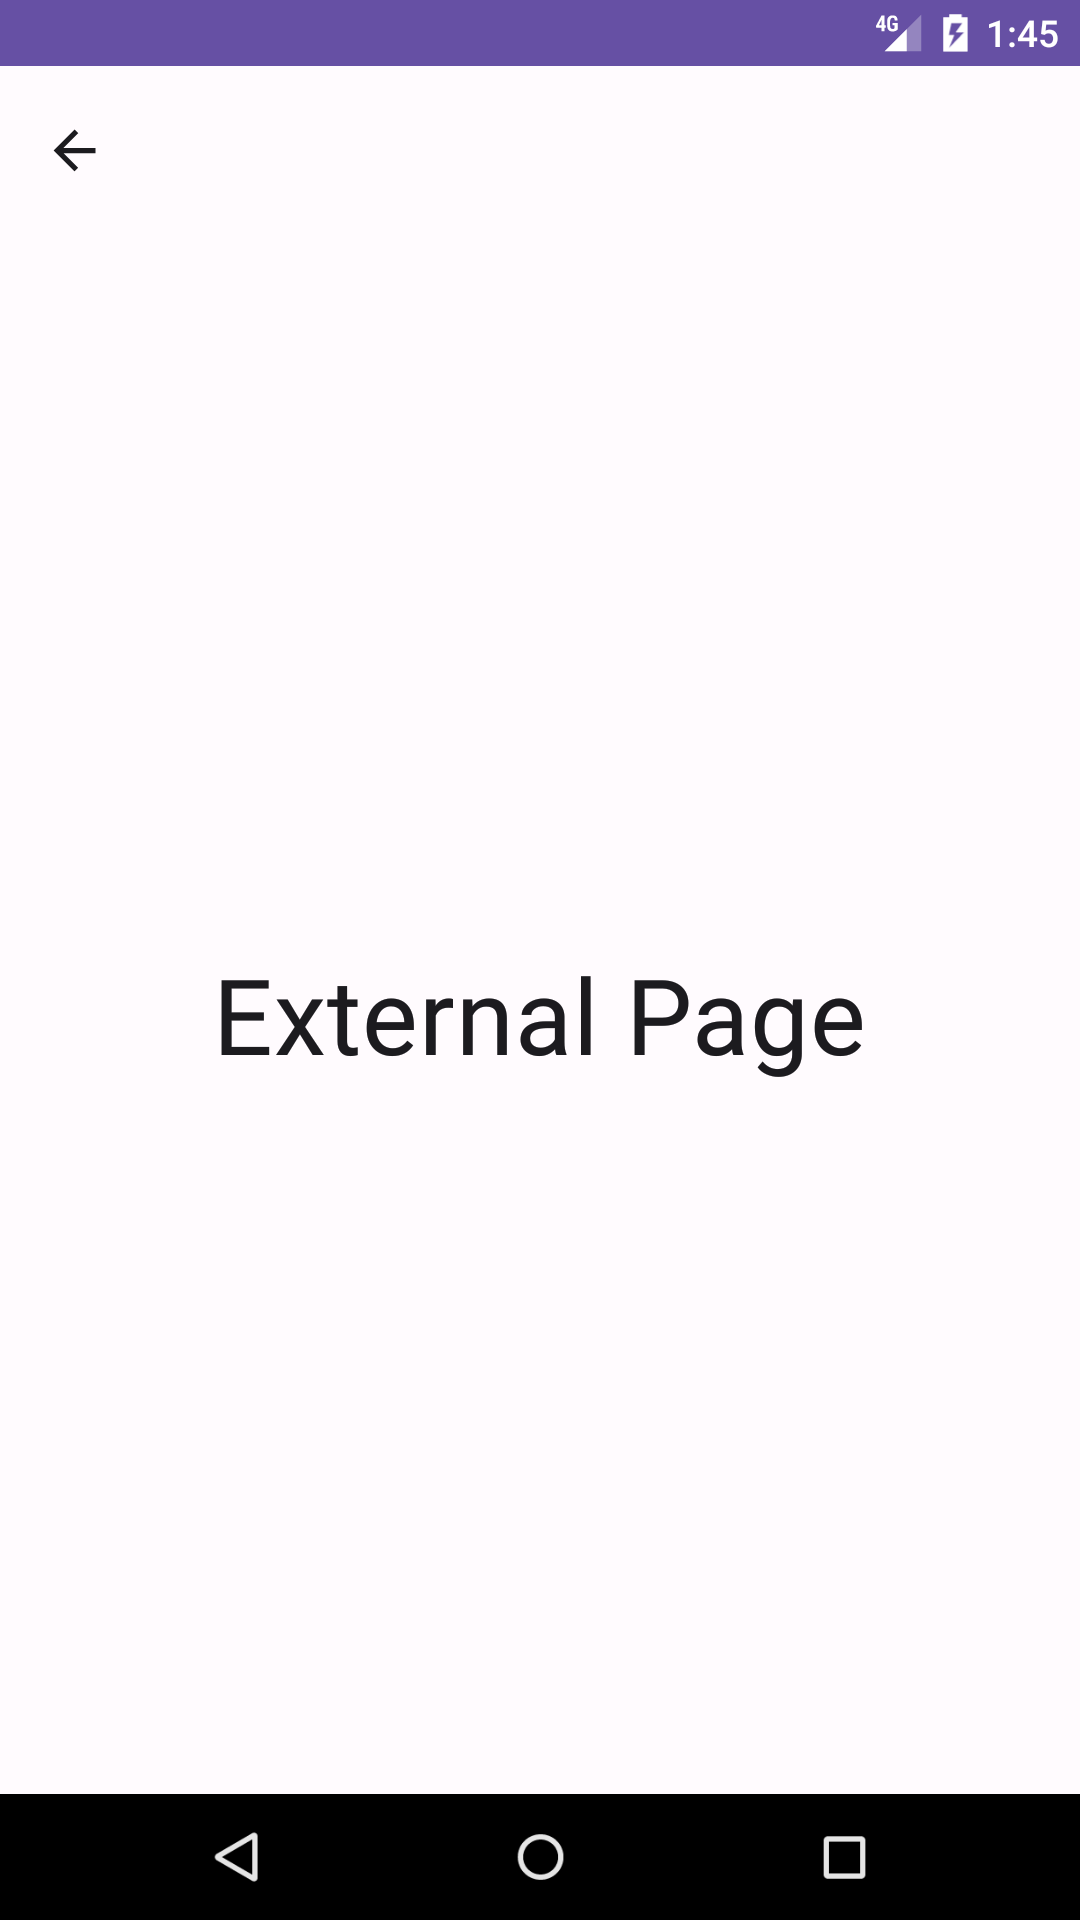
\includegraphics[height=50mm]{img/app4_2_kotlin}
    \caption{App 4 (2/3): Kotlin (Source: Own work)}
    \label{fig:app4_2_kotlin}
  \end{minipage}
  \hfill
  \begin{minipage}{.31\textwidth}
    \centering
    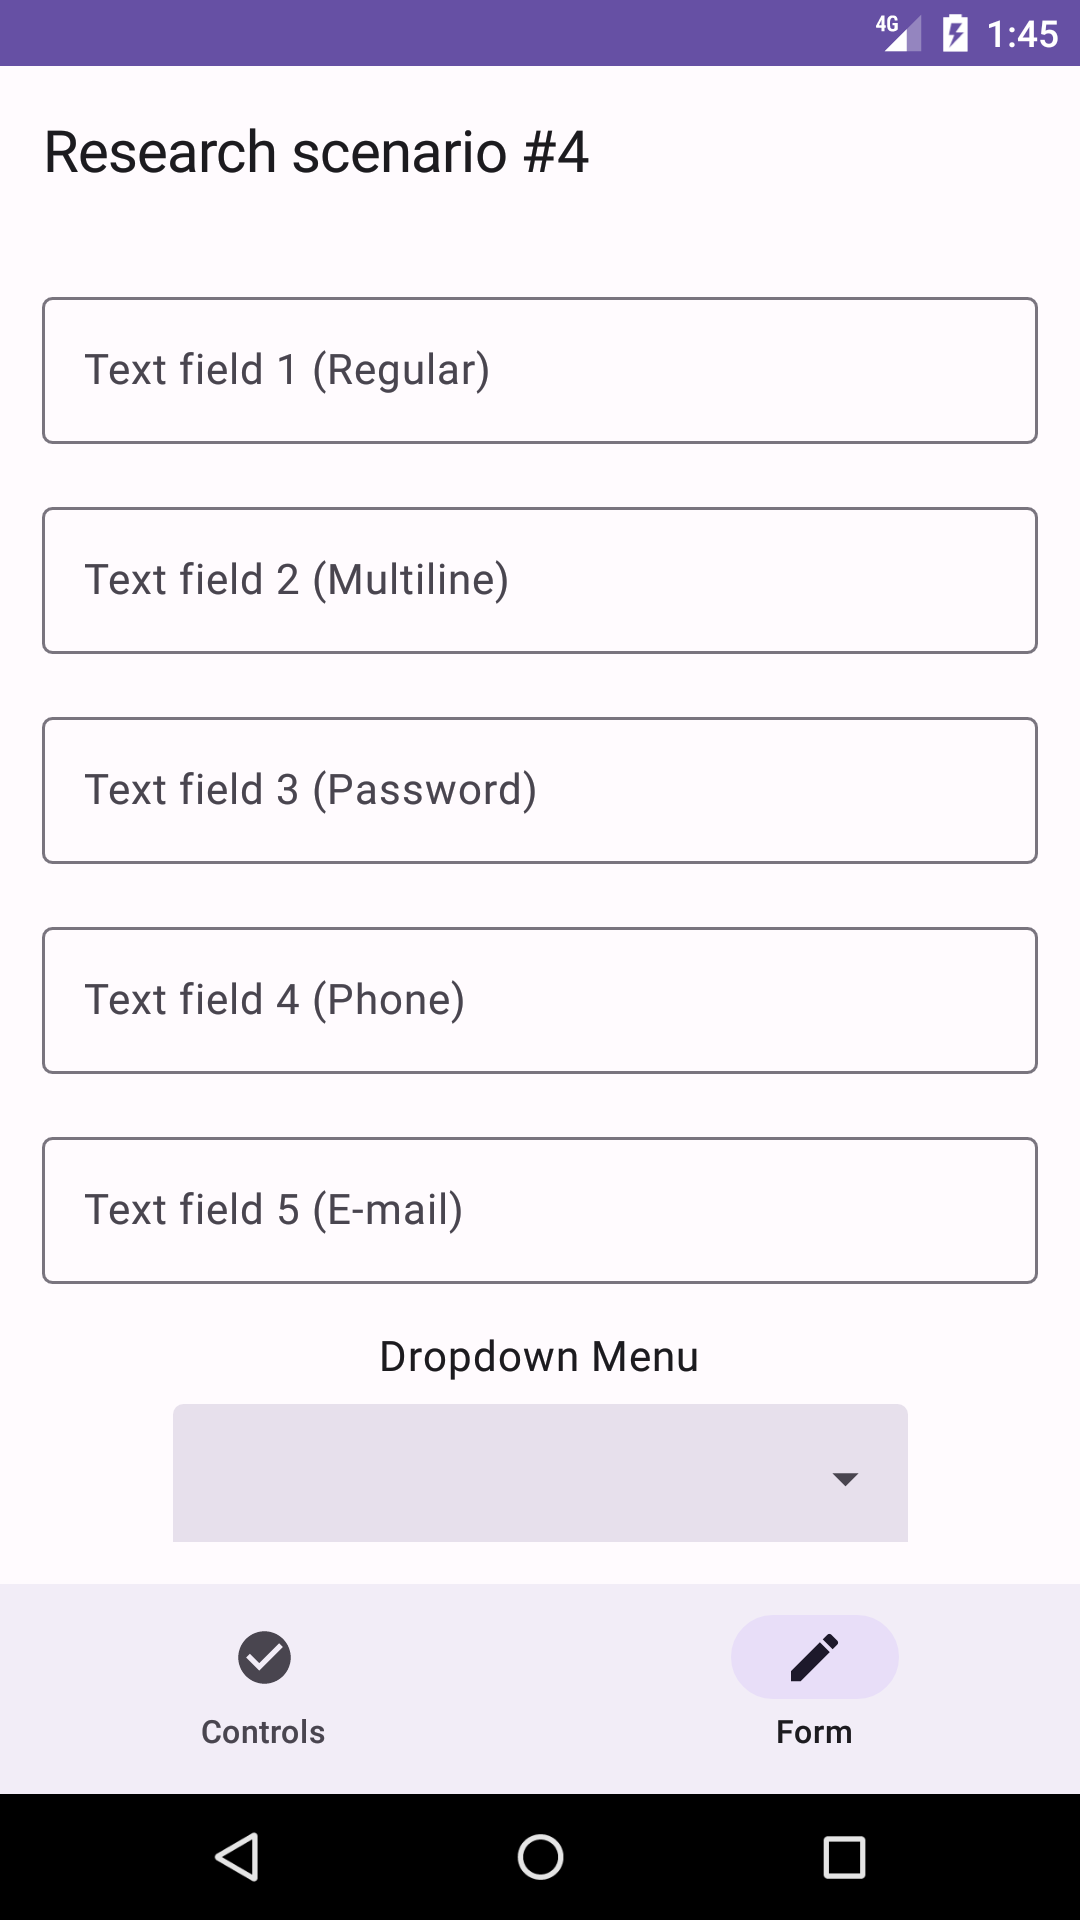
\includegraphics[height=50mm]{img/app4_3_kotlin}
    \caption{App 4 (3/3): Kotlin (Source: Own work)}
    \label{fig:app4_3_kotlin}
  \end{minipage}
\end{figure}

\begin{figure}[H]
  \begin{minipage}{.31\textwidth}
    \centering
    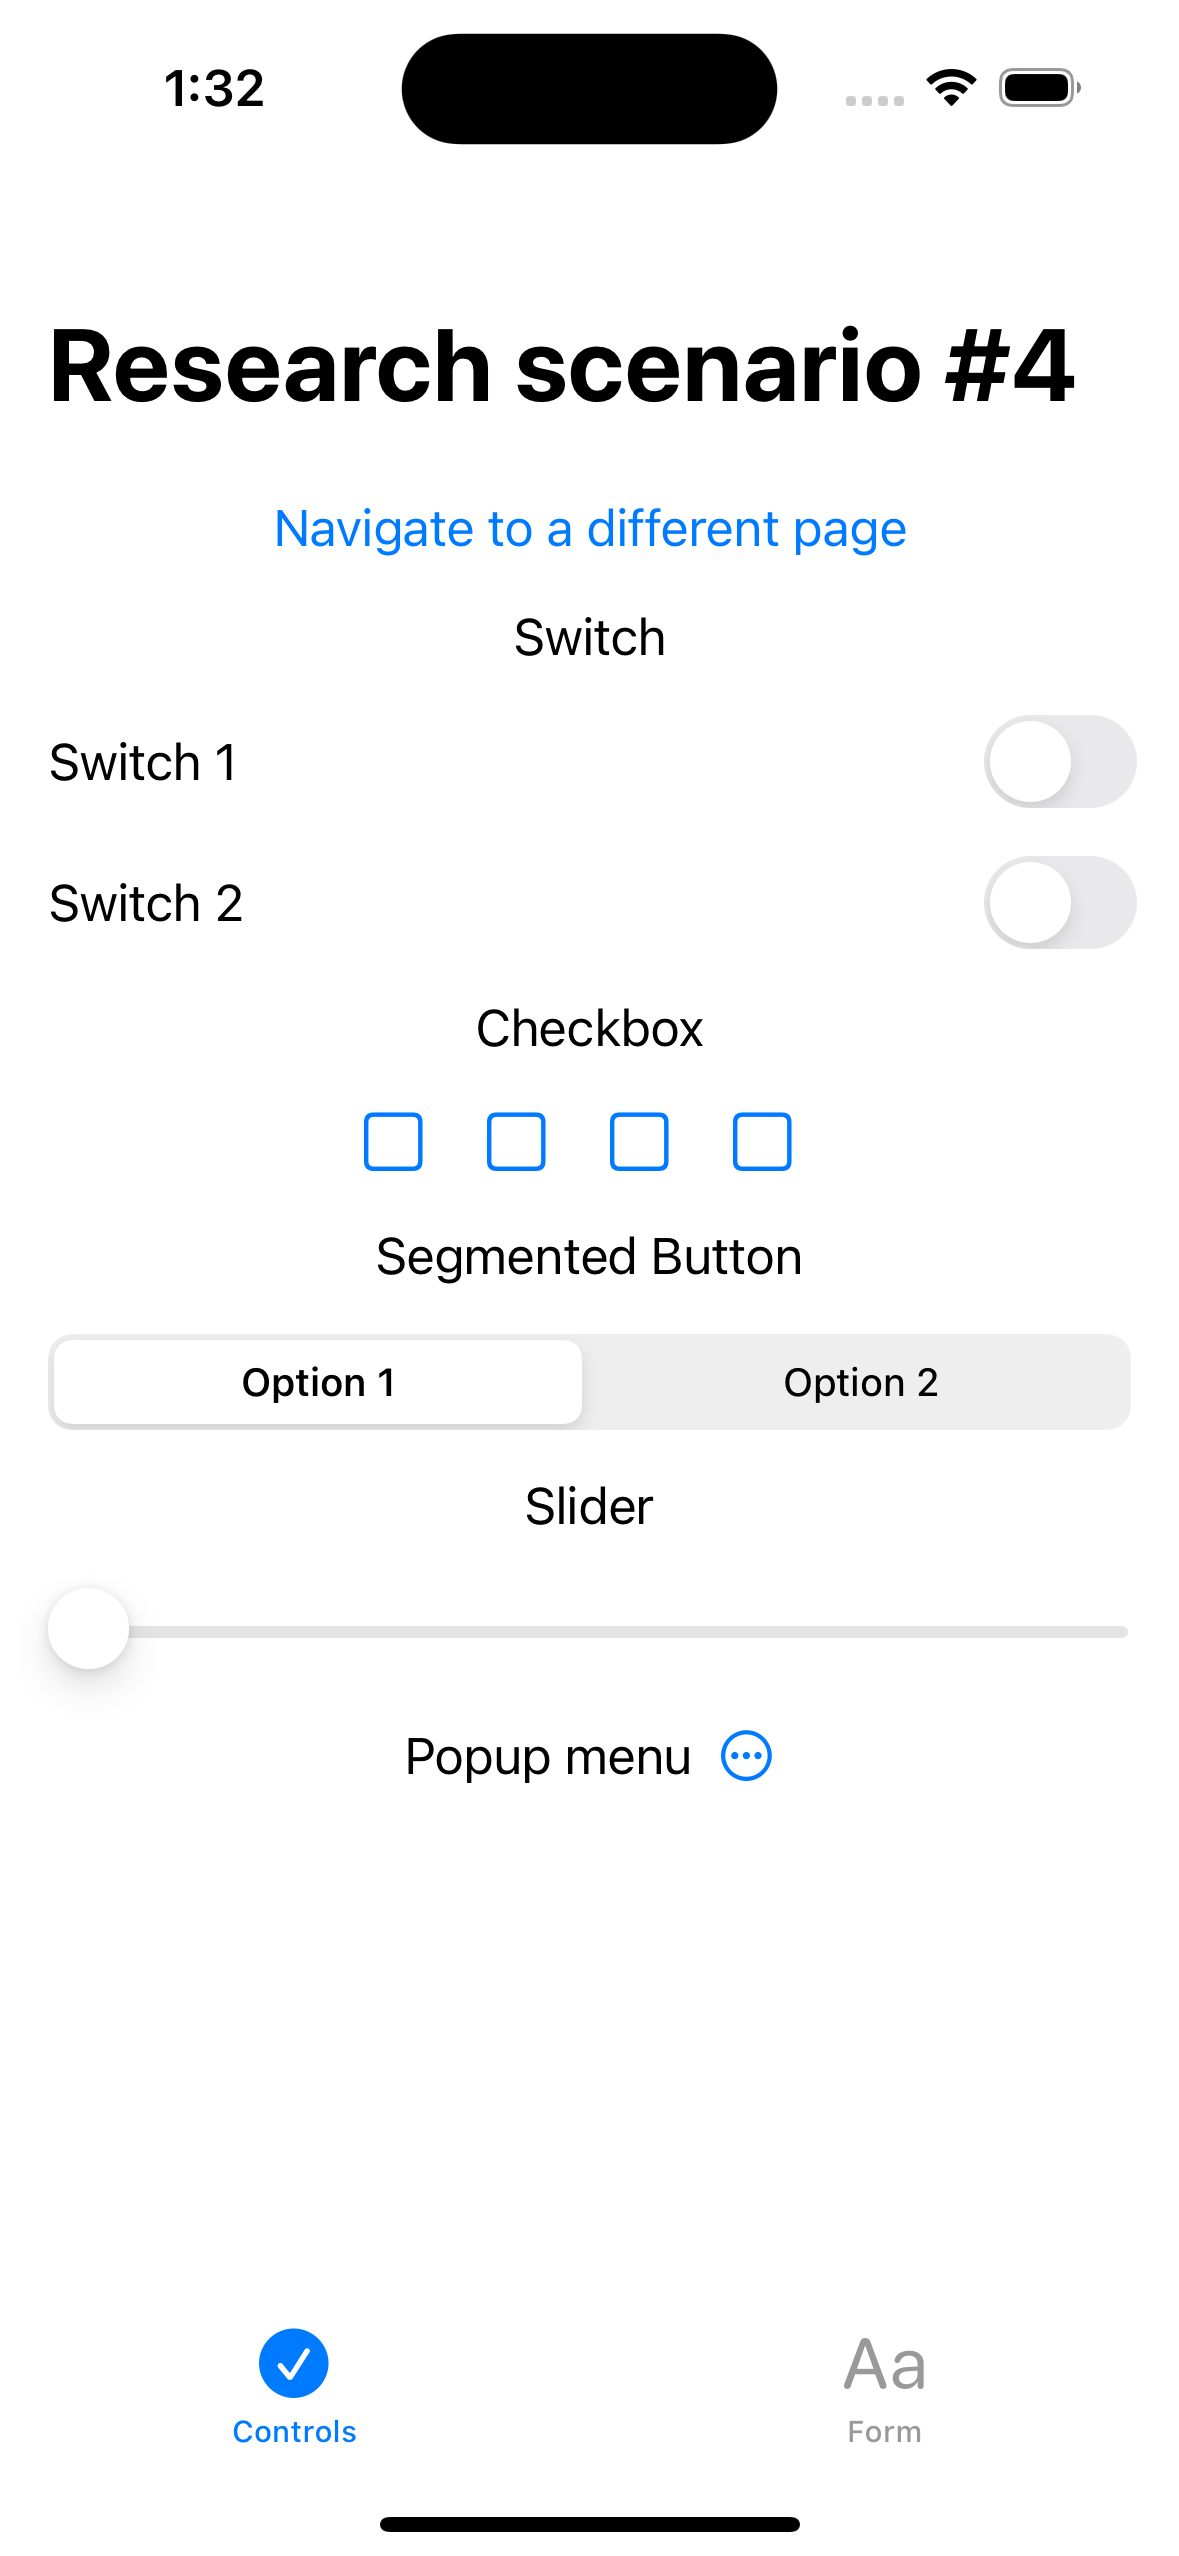
\includegraphics[height=50mm]{img/app4_1_swift}
    \caption{App 4 (1/3): Swift (Source: Own work)}
    \label{fig:app4_1_swift}
  \end{minipage}
  \hfill
  \begin{minipage}{.31\textwidth}
    \centering
    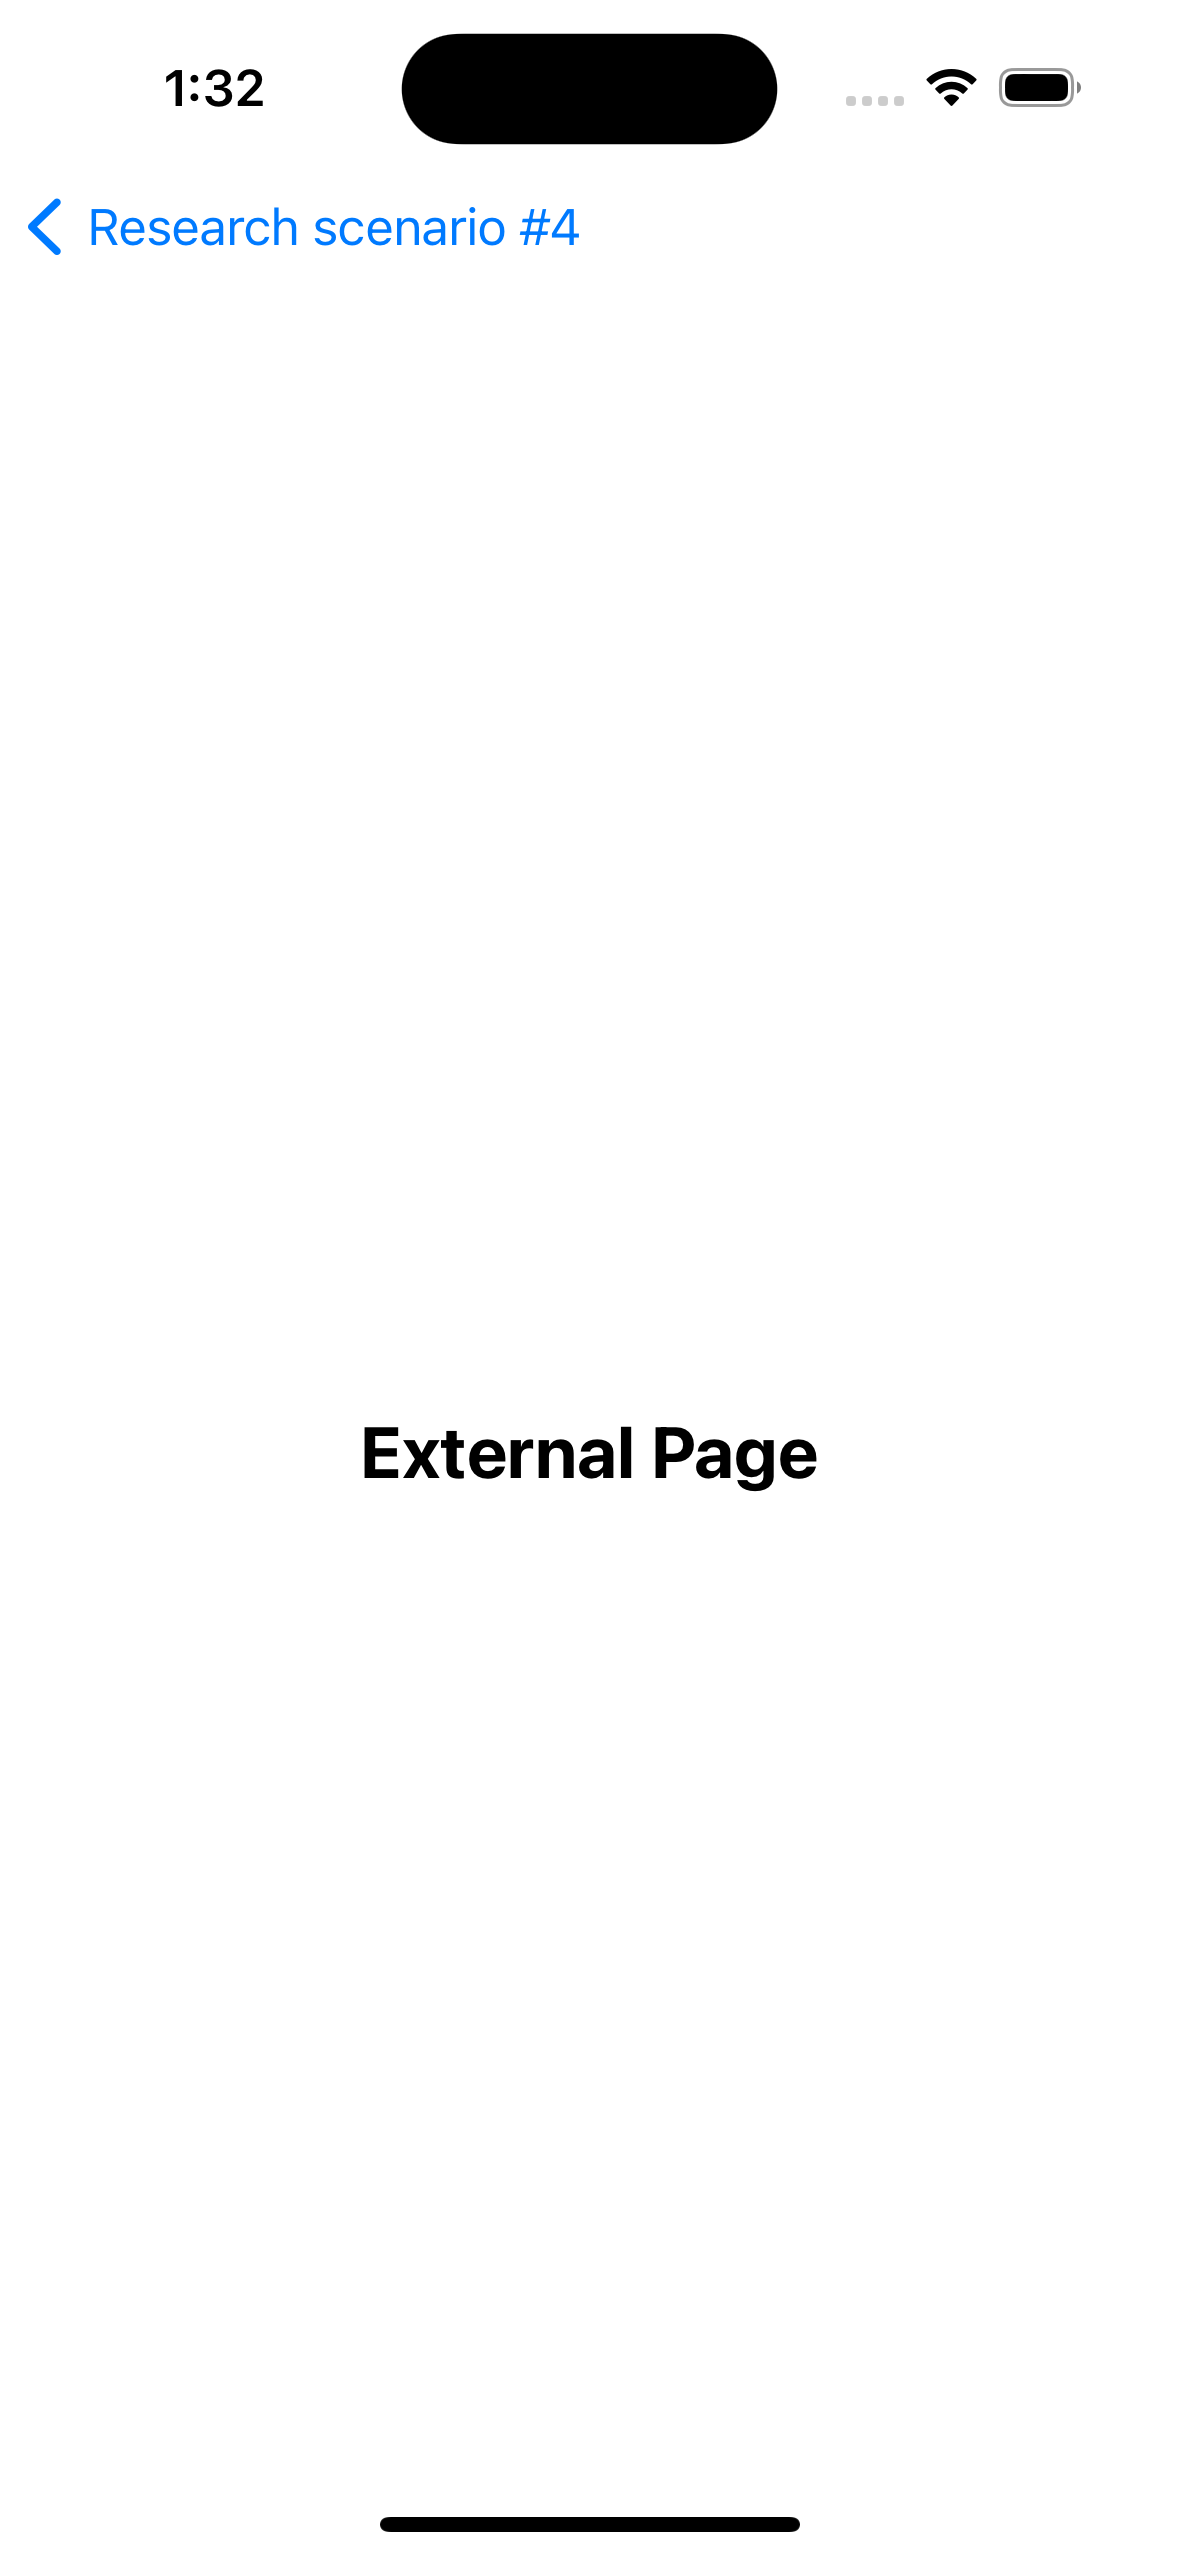
\includegraphics[height=50mm]{img/app4_2_swift}
    \caption{App 4 (2/3): Swift (Source: Own work)}
    \label{fig:app4_2_swift}
  \end{minipage}
  \hfill
  \begin{minipage}{.31\textwidth}
    \centering
    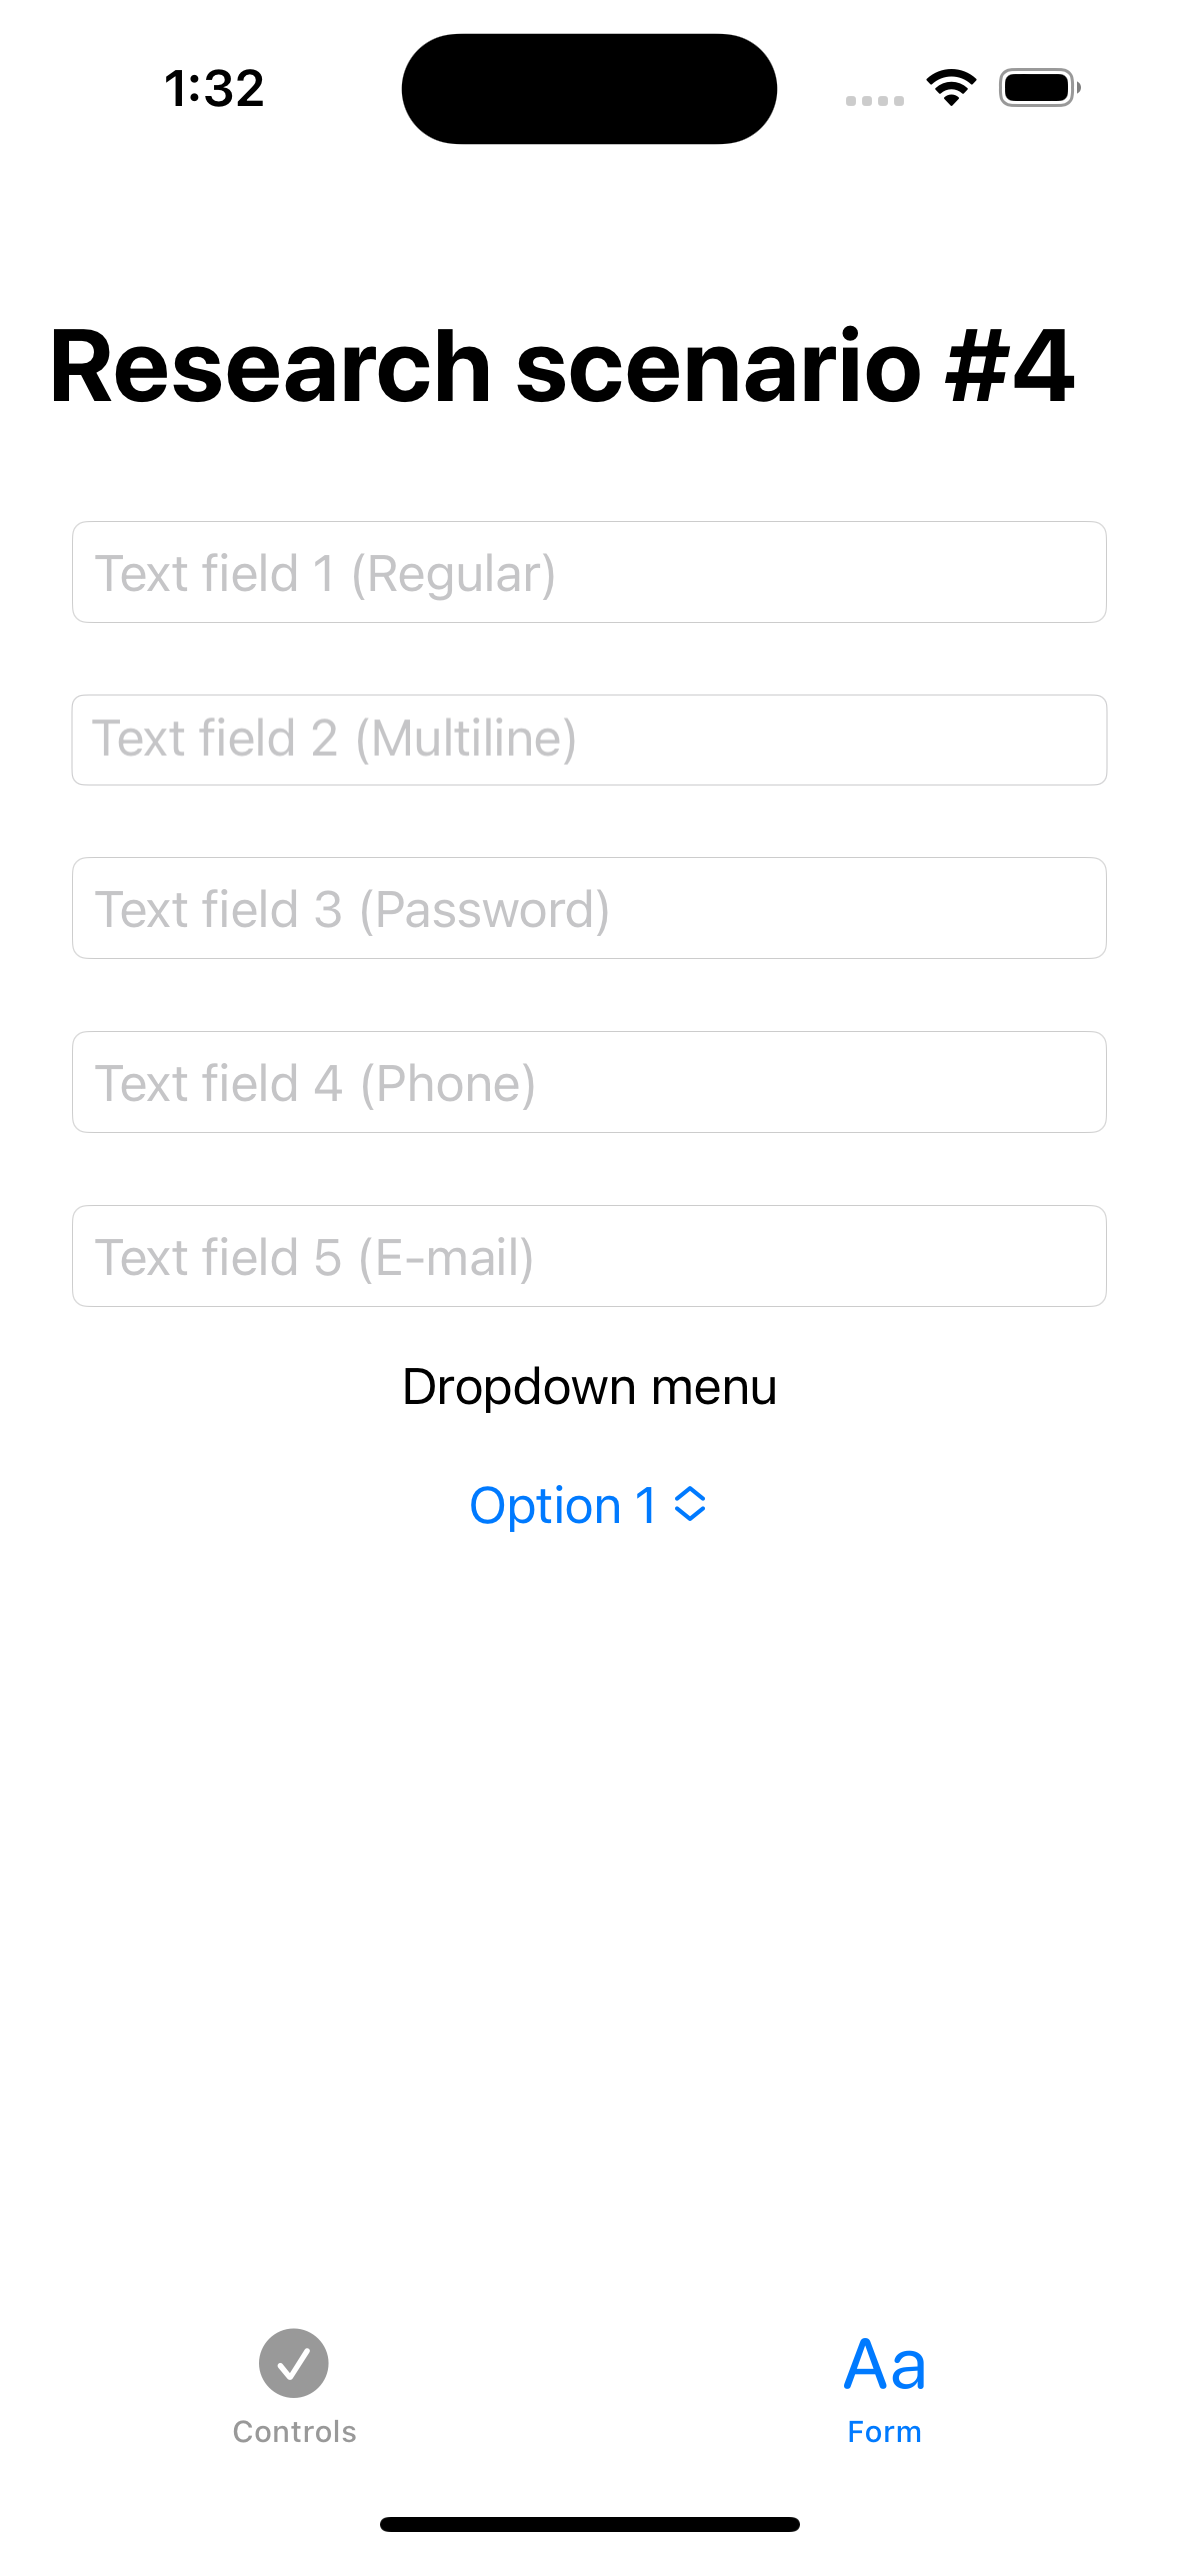
\includegraphics[height=50mm]{img/app4_3_swift}
    \caption{App 4 (3/3): Swift (Source: Own work)}
    \label{fig:app4_3_swift}
  \end{minipage}
\end{figure}

\begin{figure}[H]
  \begin{minipage}{.31\textwidth}
    \centering
    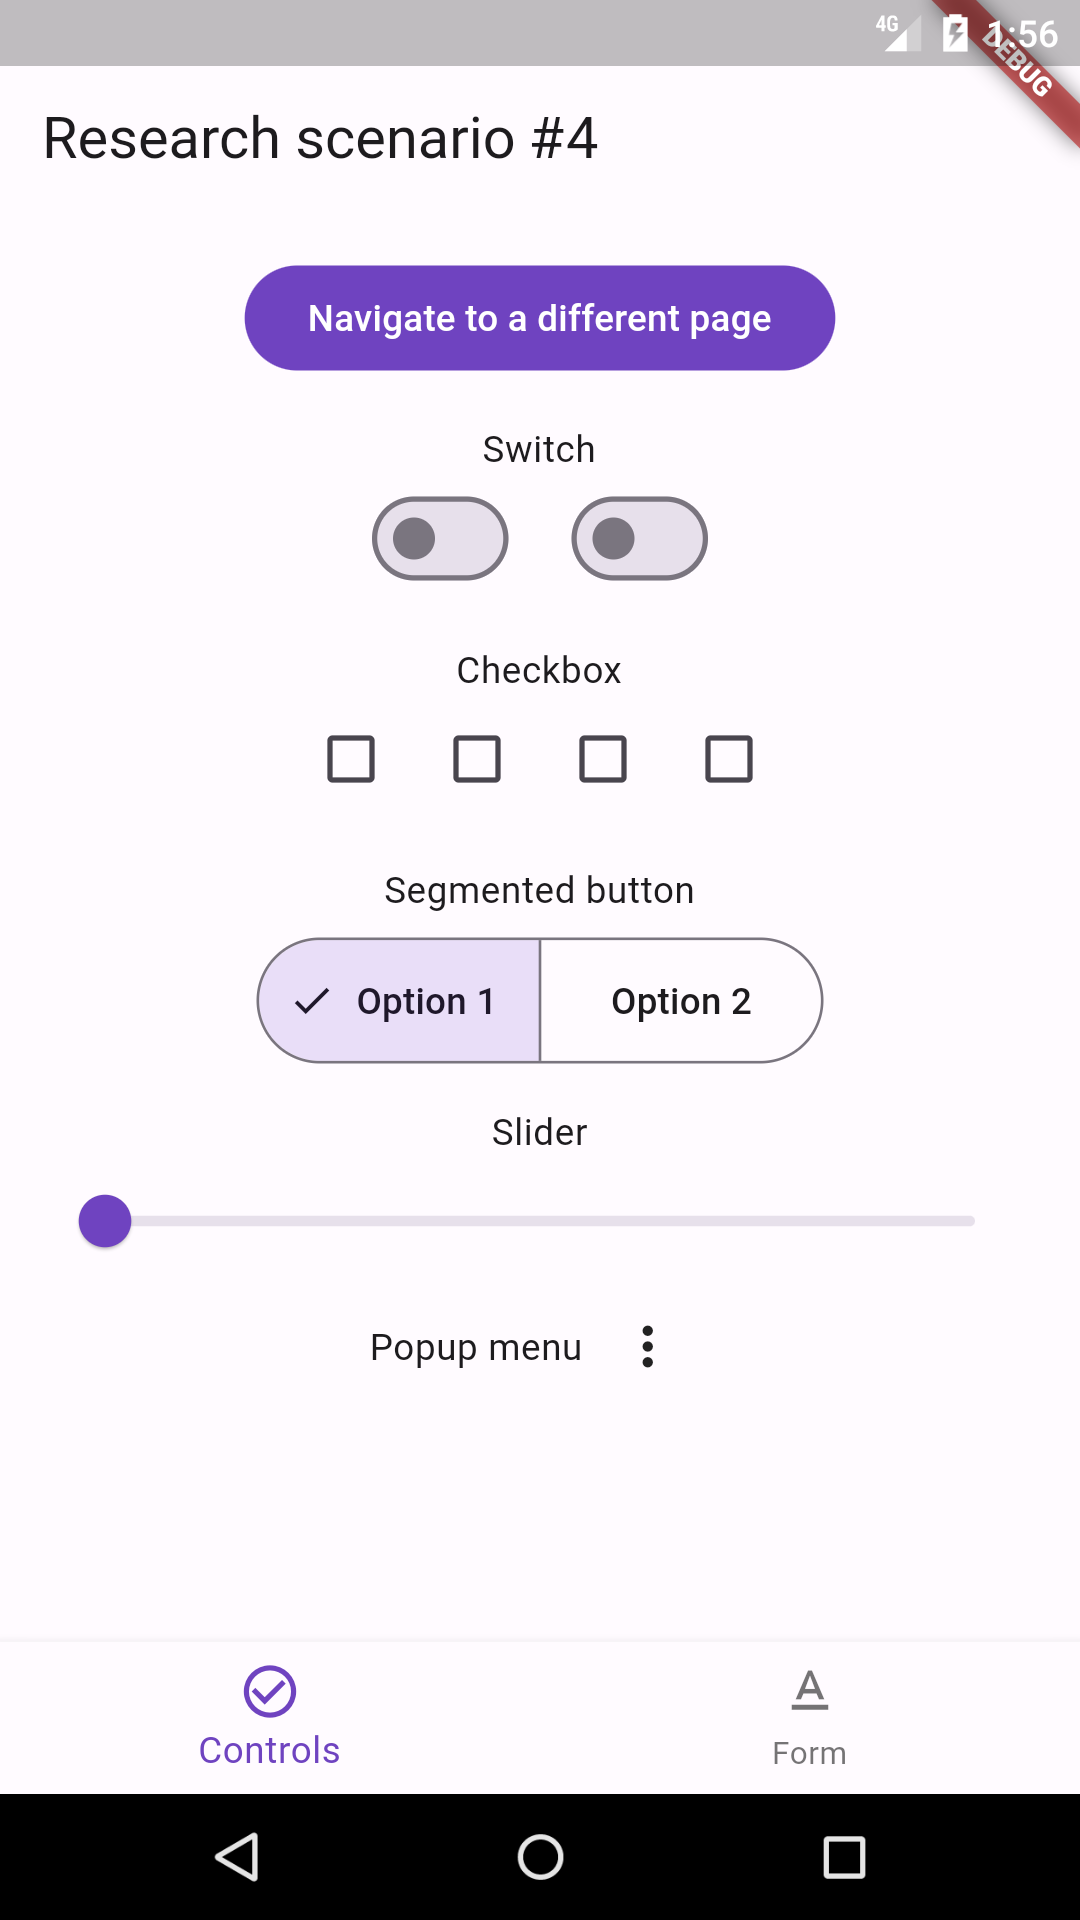
\includegraphics[height=50mm]{img/app4_1_flutter_android}
    \caption{App 4 (1/3): Flutter Android (Source: Own work)}
    \label{fig:app4_1_flutter_android}
  \end{minipage}
  \hfill
  \begin{minipage}{.31\textwidth}
    \centering
    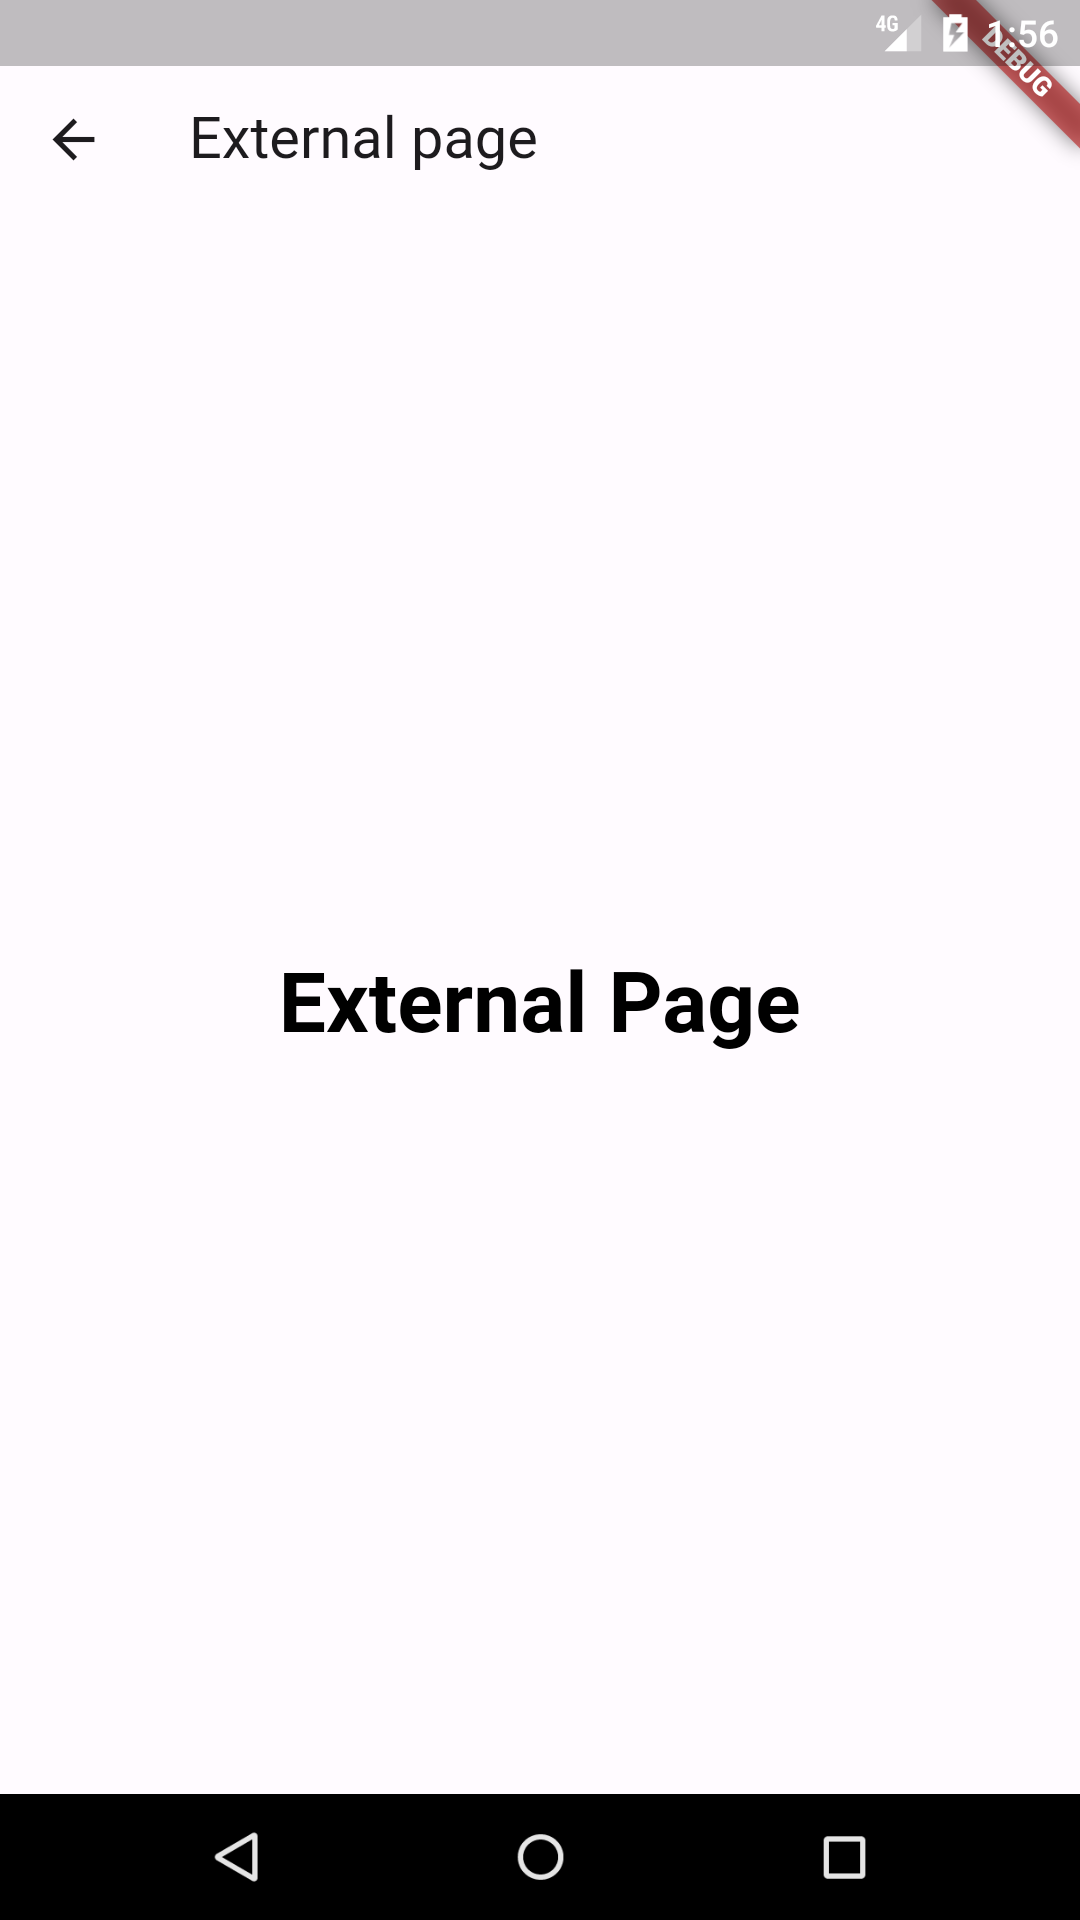
\includegraphics[height=50mm]{img/app4_2_flutter_android}
    \caption{App 4 (2/3): Flutter Android (Source: Own work)}
    \label{fig:app4_2_flutter_android}
  \end{minipage}
  \hfill
  \begin{minipage}{.31\textwidth}
    \centering
    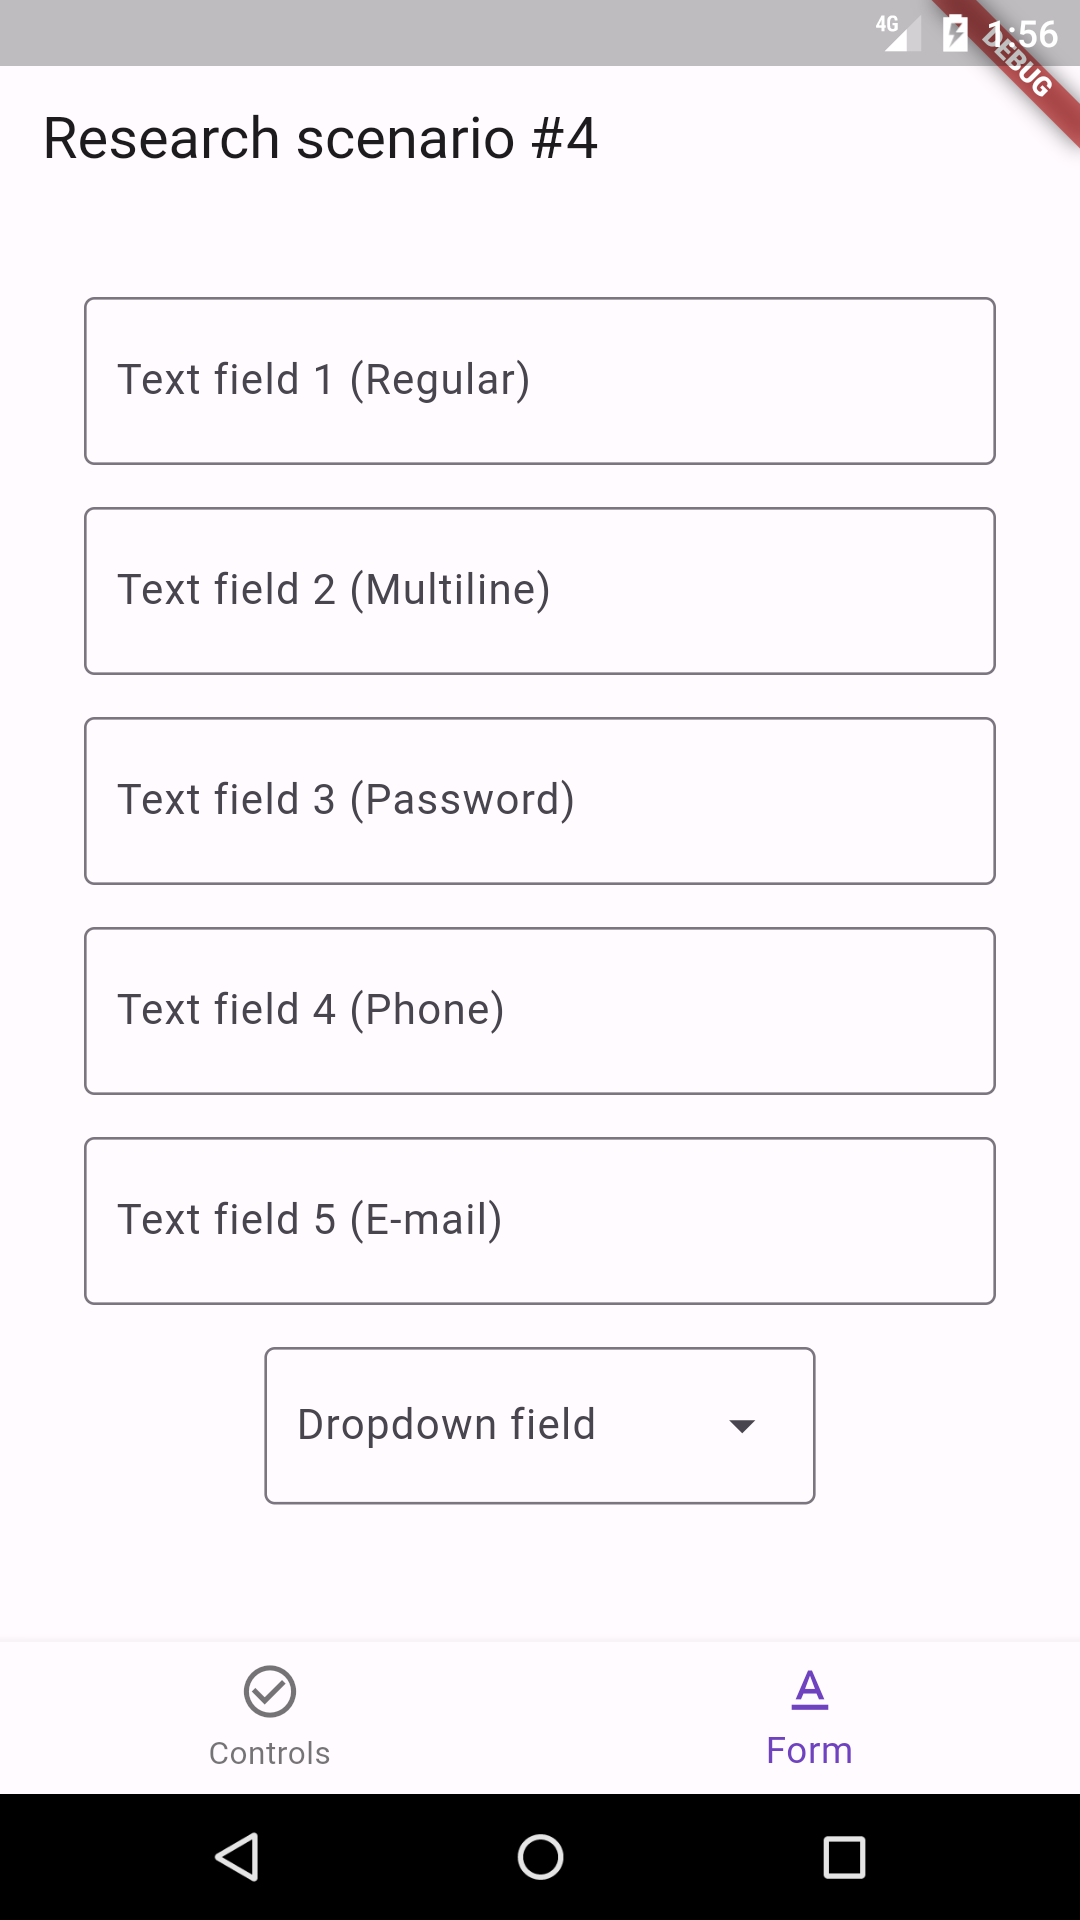
\includegraphics[height=50mm]{img/app4_3_flutter_android}
    \caption{App 4 (3/3): Flutter Android (Source: Own work)}
    \label{fig:app4_3_flutter_android}
  \end{minipage}
\end{figure}

\begin{figure}[H]
  \begin{minipage}{.31\textwidth}
    \centering
    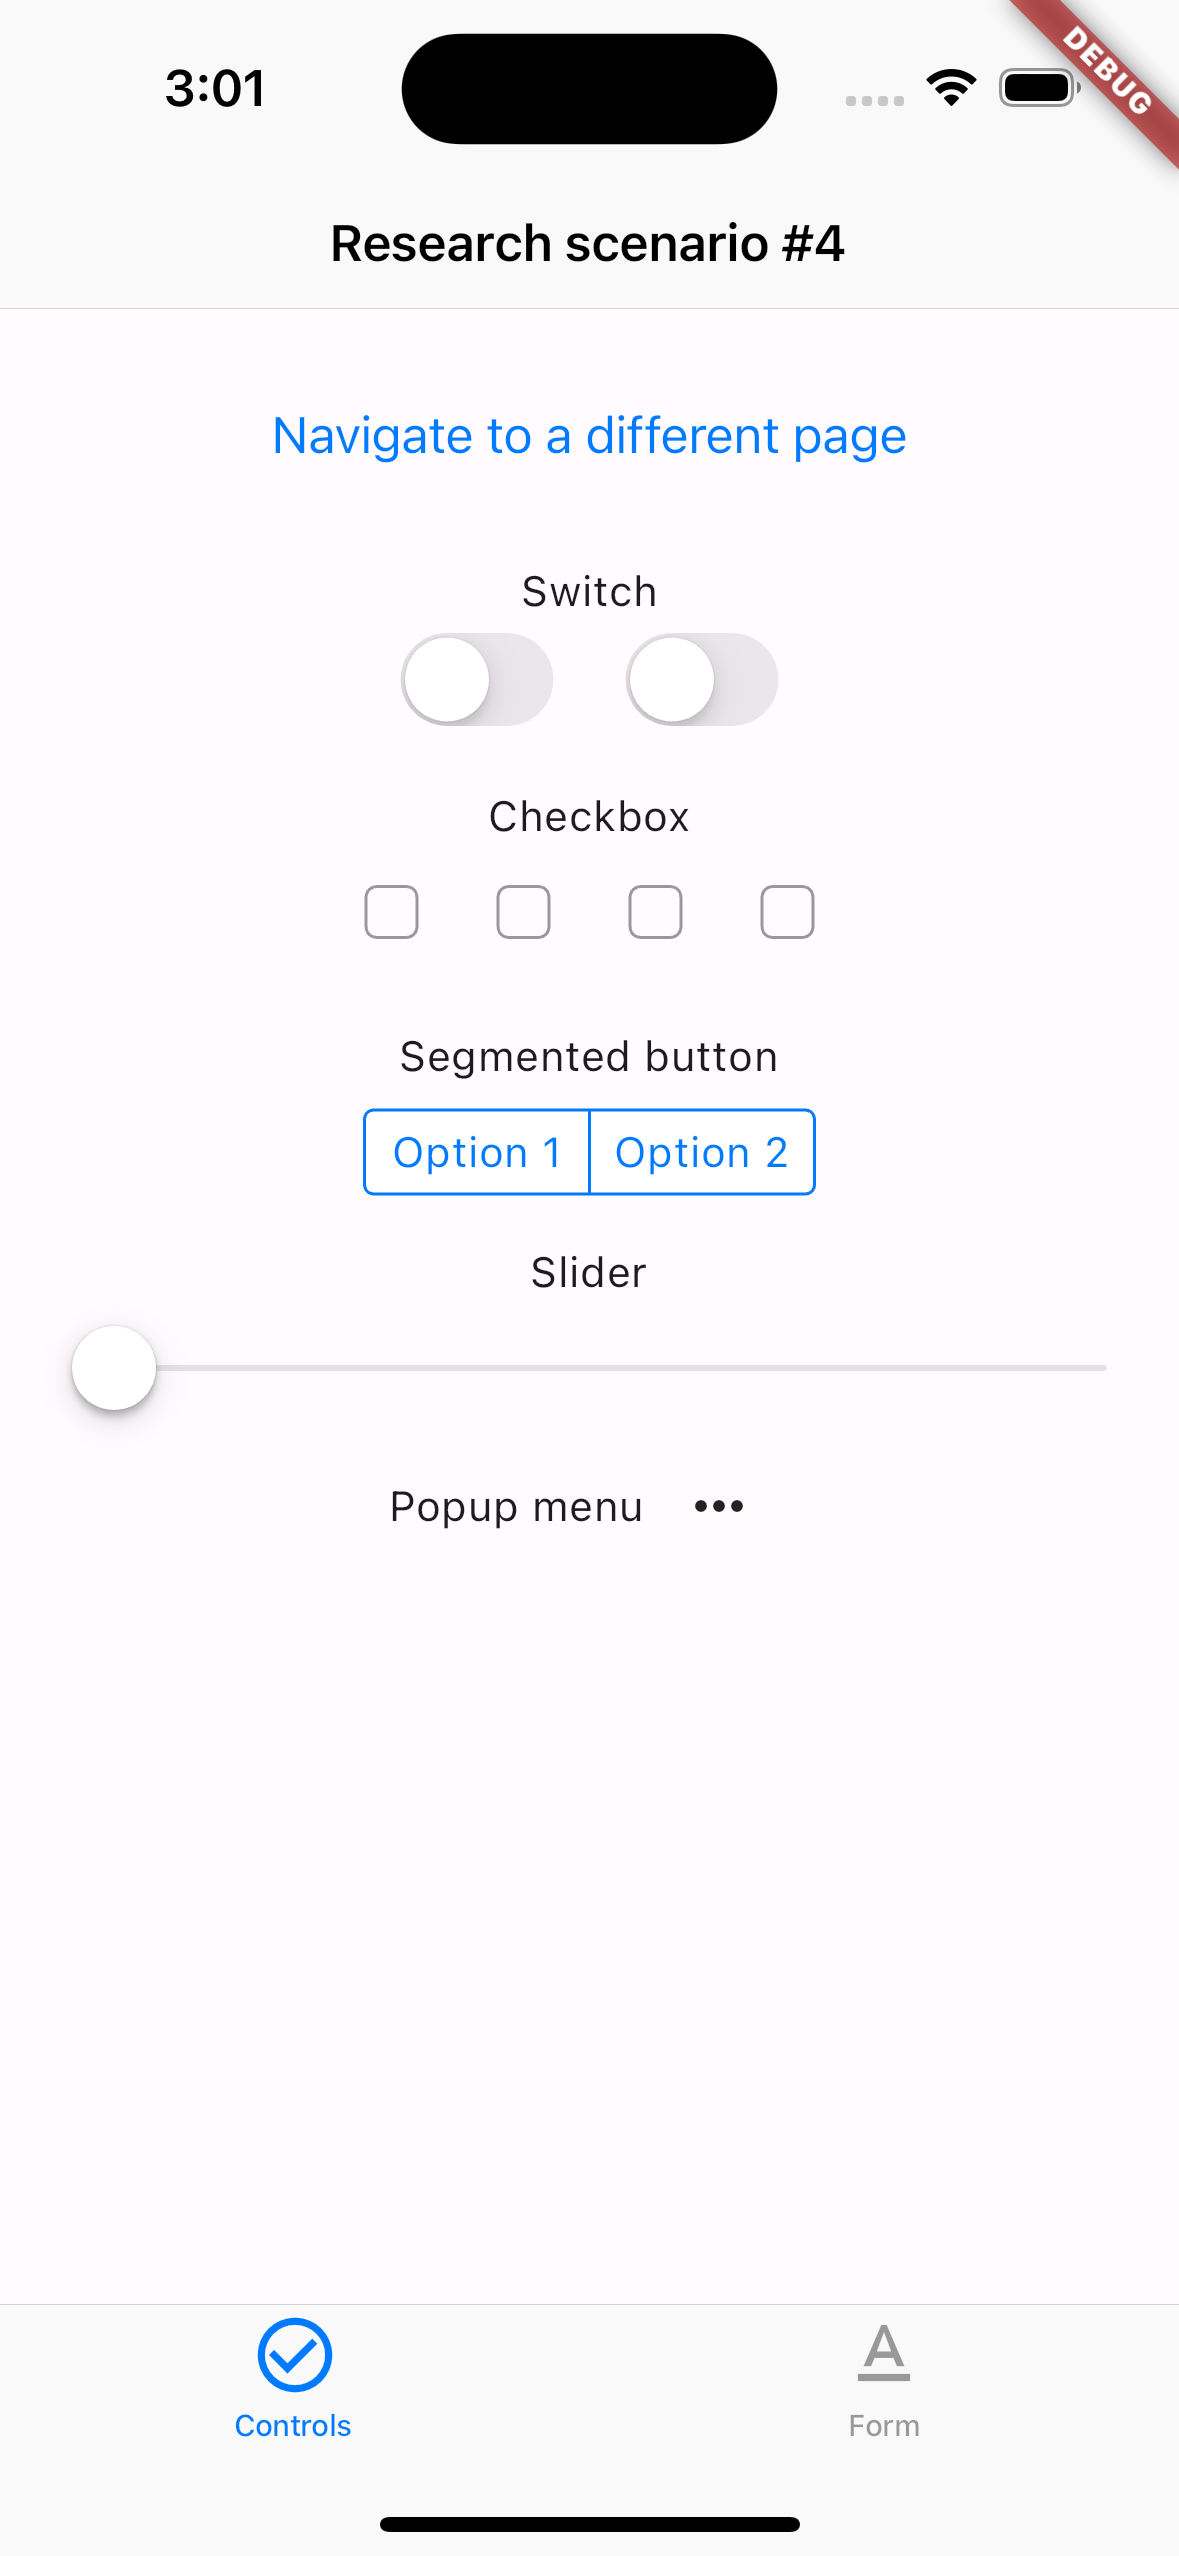
\includegraphics[height=50mm]{img/app4_1_flutter_ios}
    \caption{App 4 (1/3): Flutter iOS (Source: Own work)}
    \label{fig:app4_1_flutter_ios}
  \end{minipage}
  \hfill
  \begin{minipage}{.31\textwidth}
    \centering
    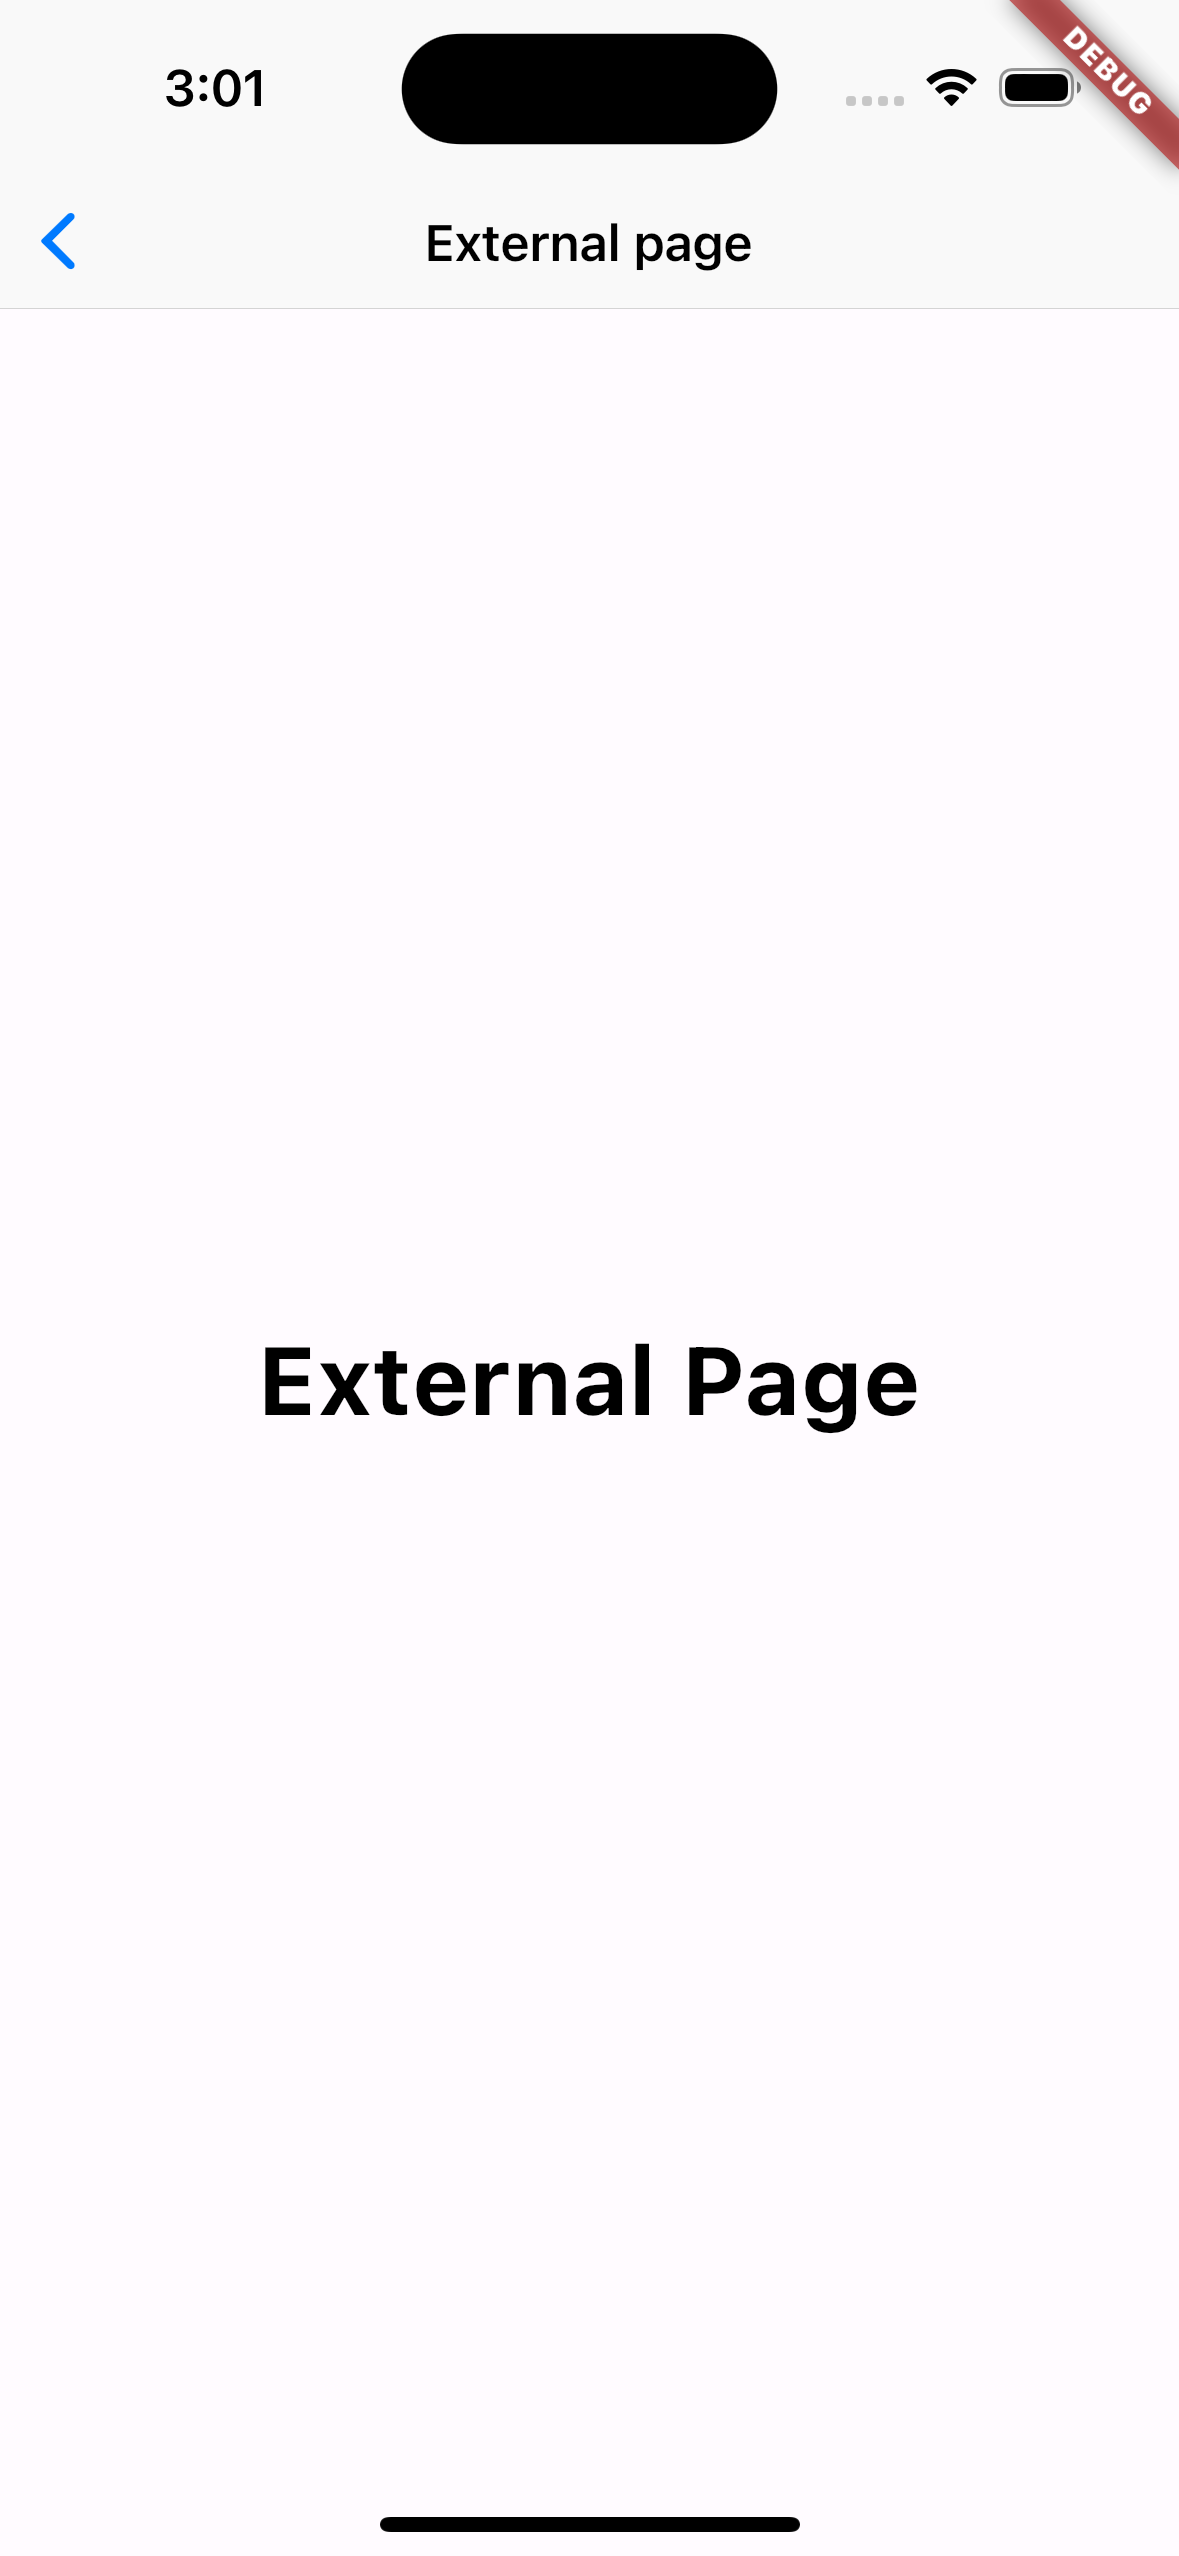
\includegraphics[height=50mm]{img/app4_2_flutter_ios}
    \caption{App 4 (2/3): Flutter iOS (Source: Own work)}
    \label{fig:app4_2_flutter_ios}
  \end{minipage}
  \hfill
  \begin{minipage}{.31\textwidth}
    \centering
    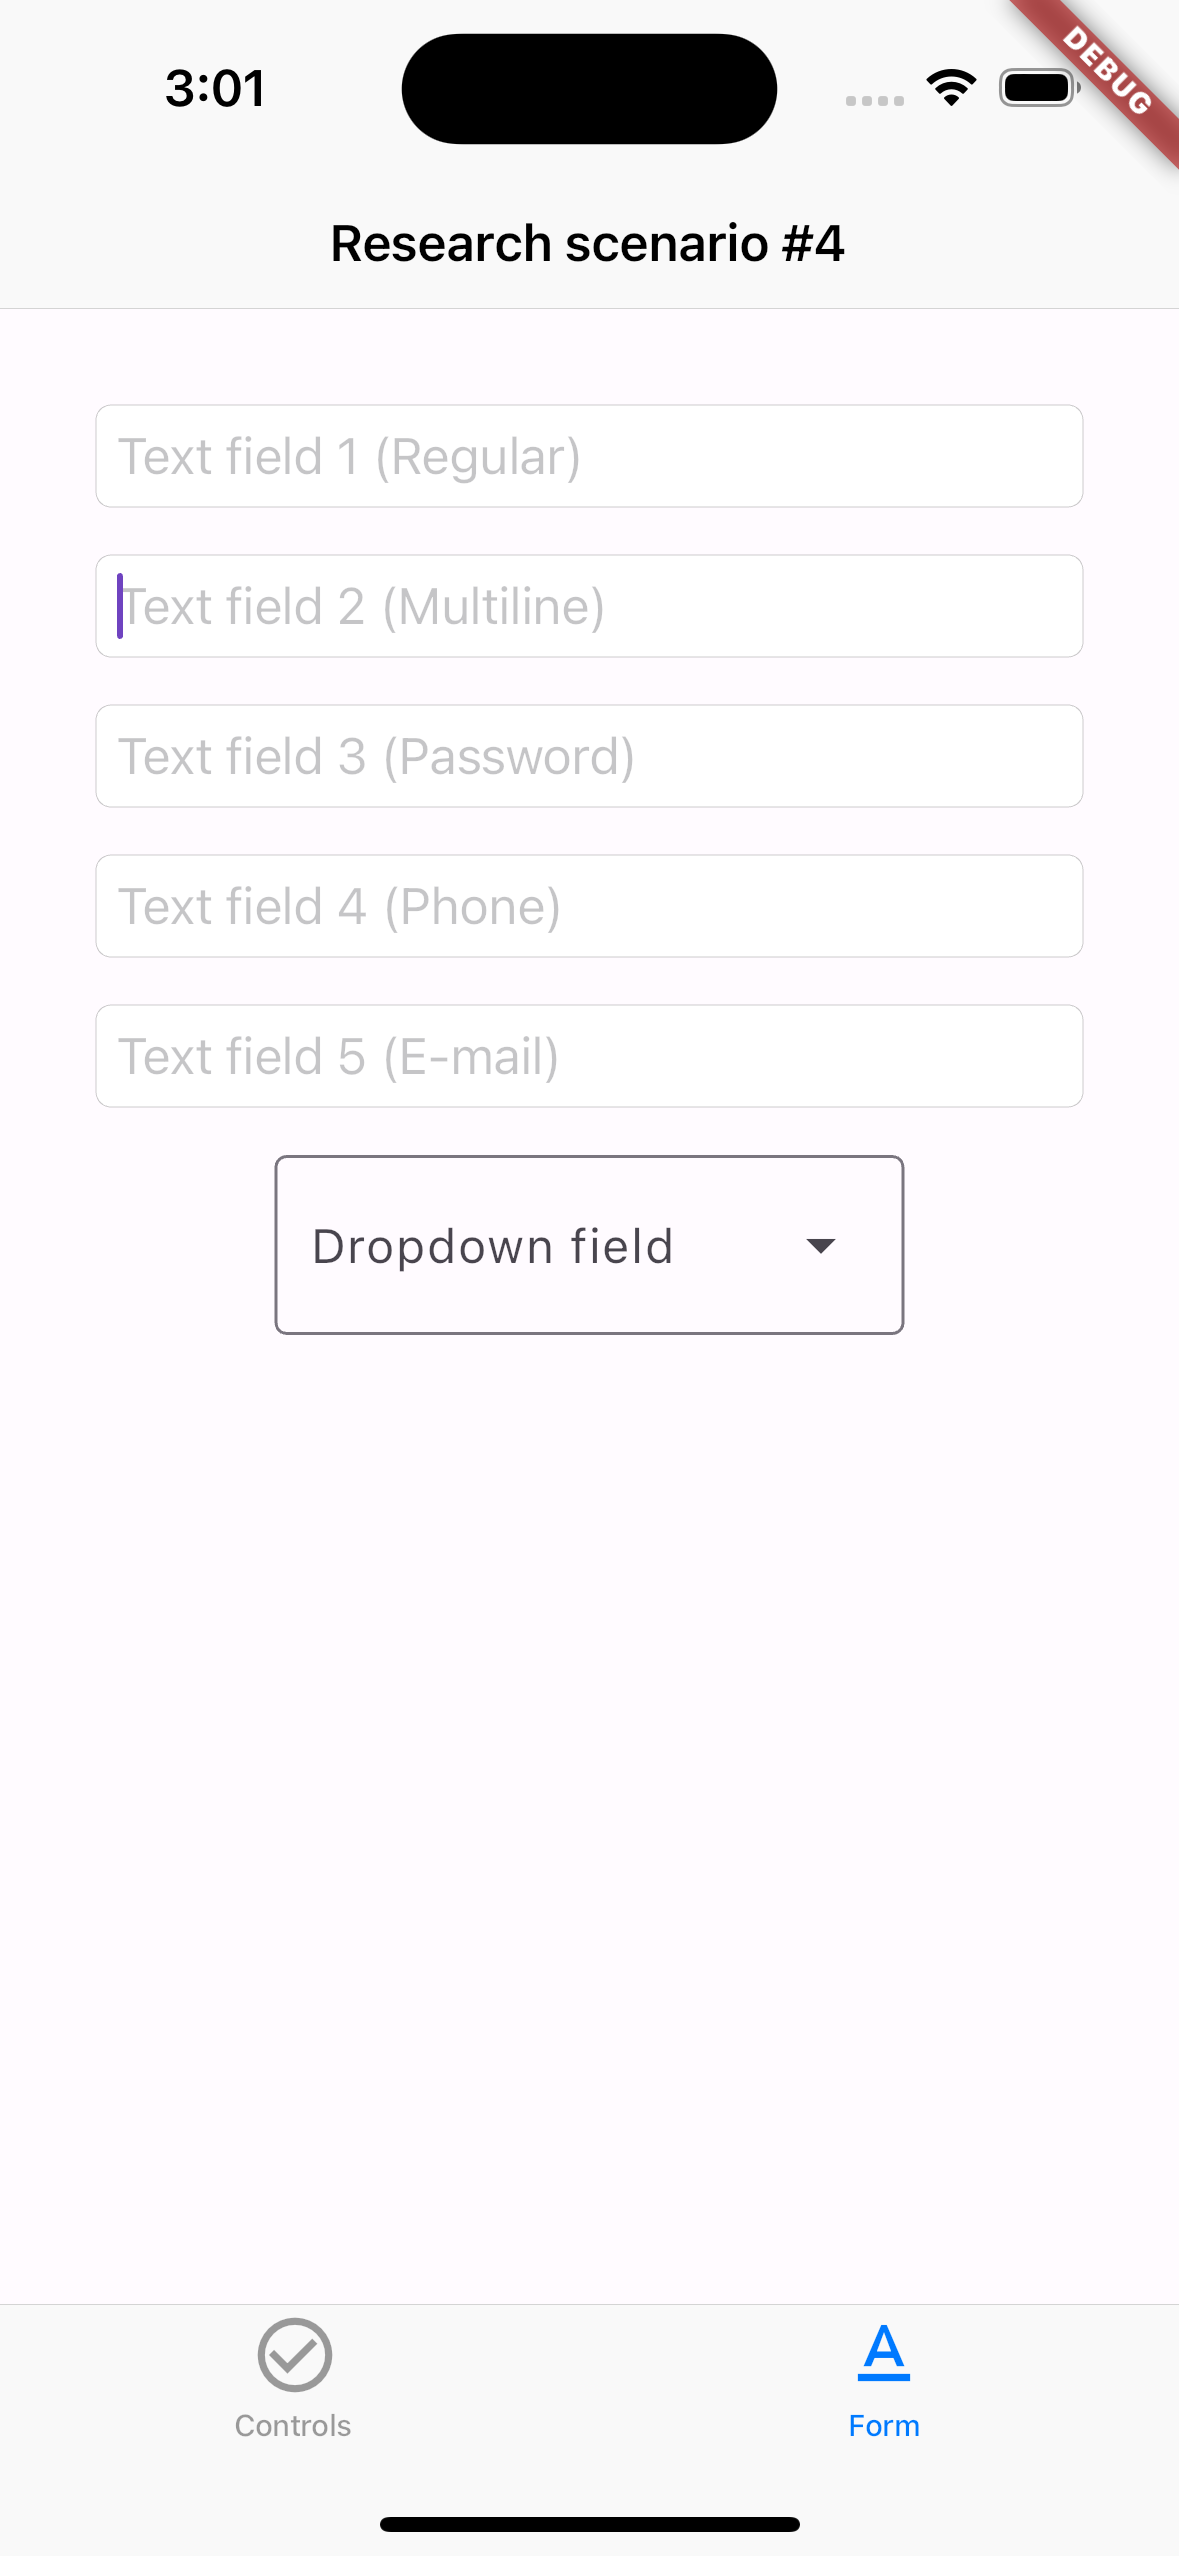
\includegraphics[height=50mm]{img/app4_3_flutter_ios}
    \caption{App 4 (3/3): Flutter iOS (Source: Own work)}
    \label{fig:app4_3_flutter_ios}
  \end{minipage}
\end{figure}

\begin{figure}[H]
  \begin{minipage}{.31\textwidth}
    \centering
    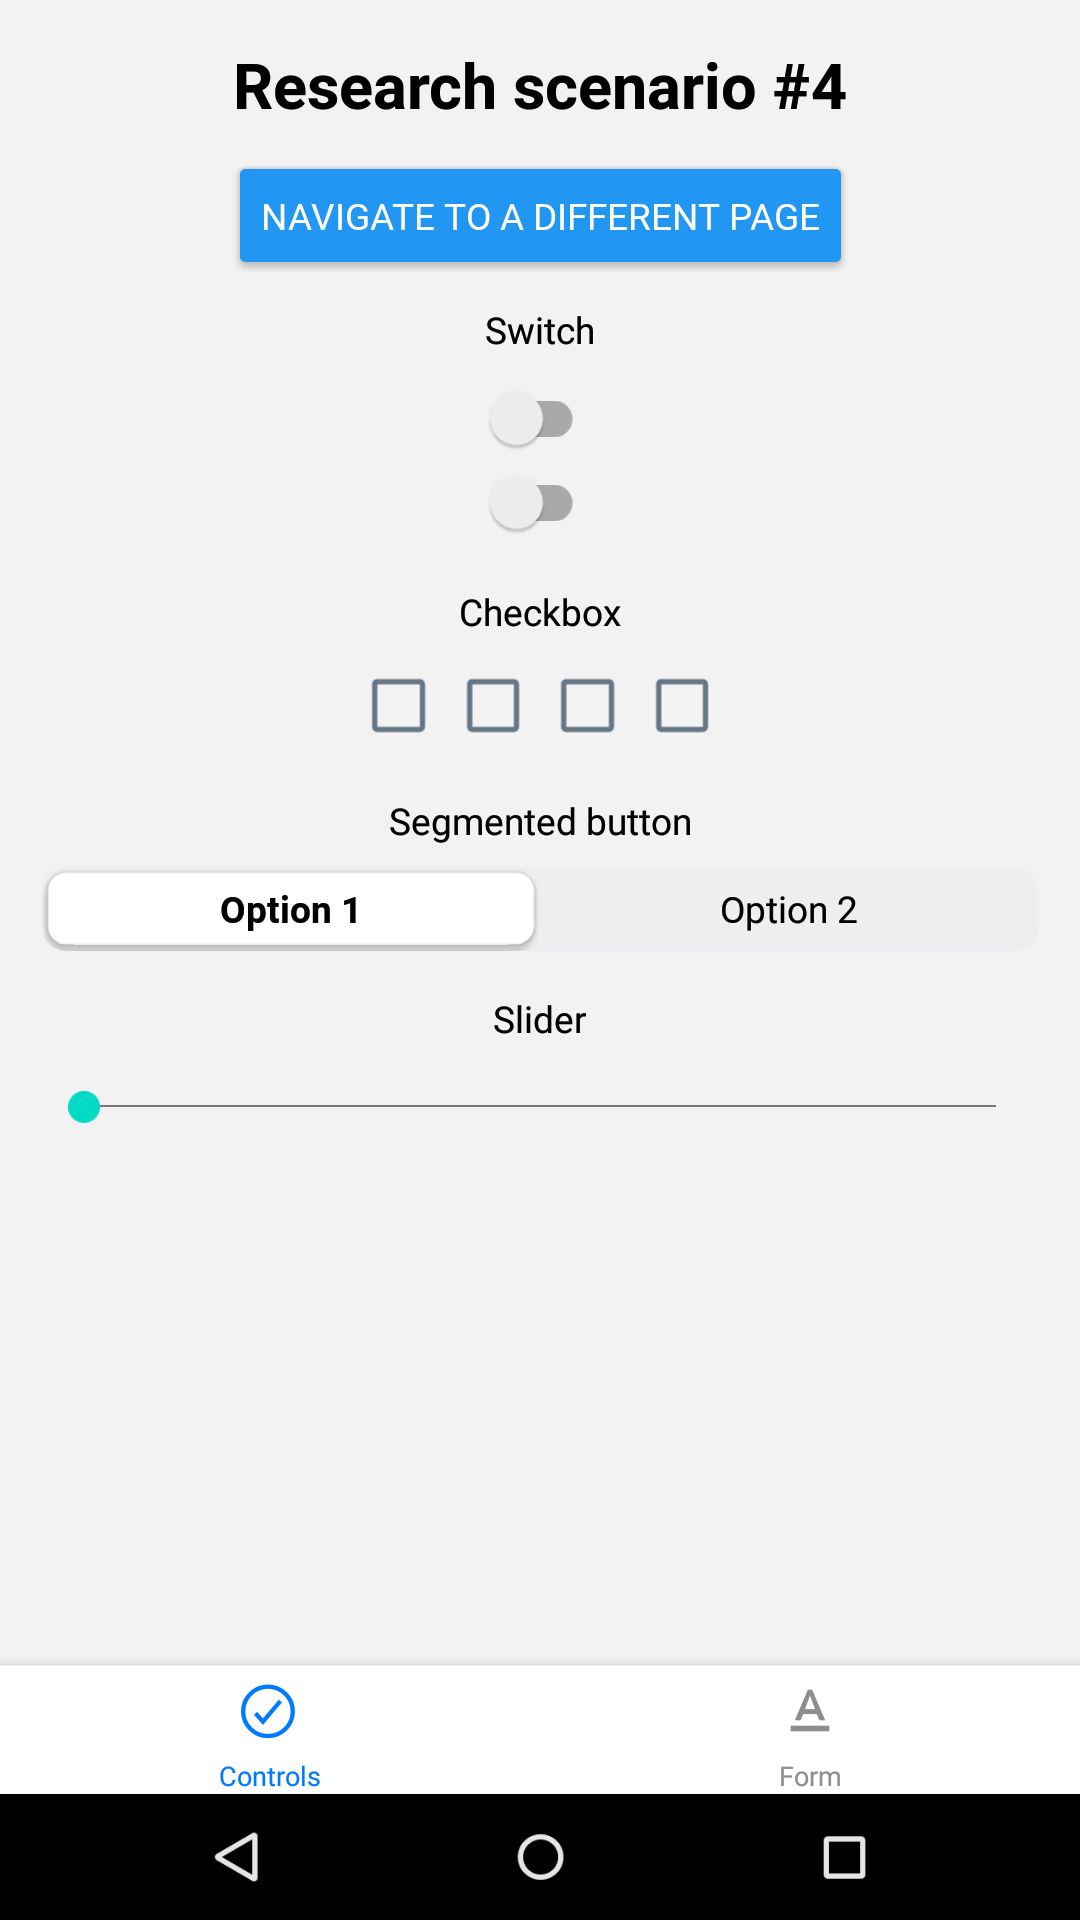
\includegraphics[height=50mm]{img/app4_1_rn_android}
    \caption{App 4 (1/3): React Native Android (Source: Own work)}
    \label{fig:app4_1_rn_android}
  \end{minipage}
  \hfill
  \begin{minipage}{.31\textwidth}
    \centering
    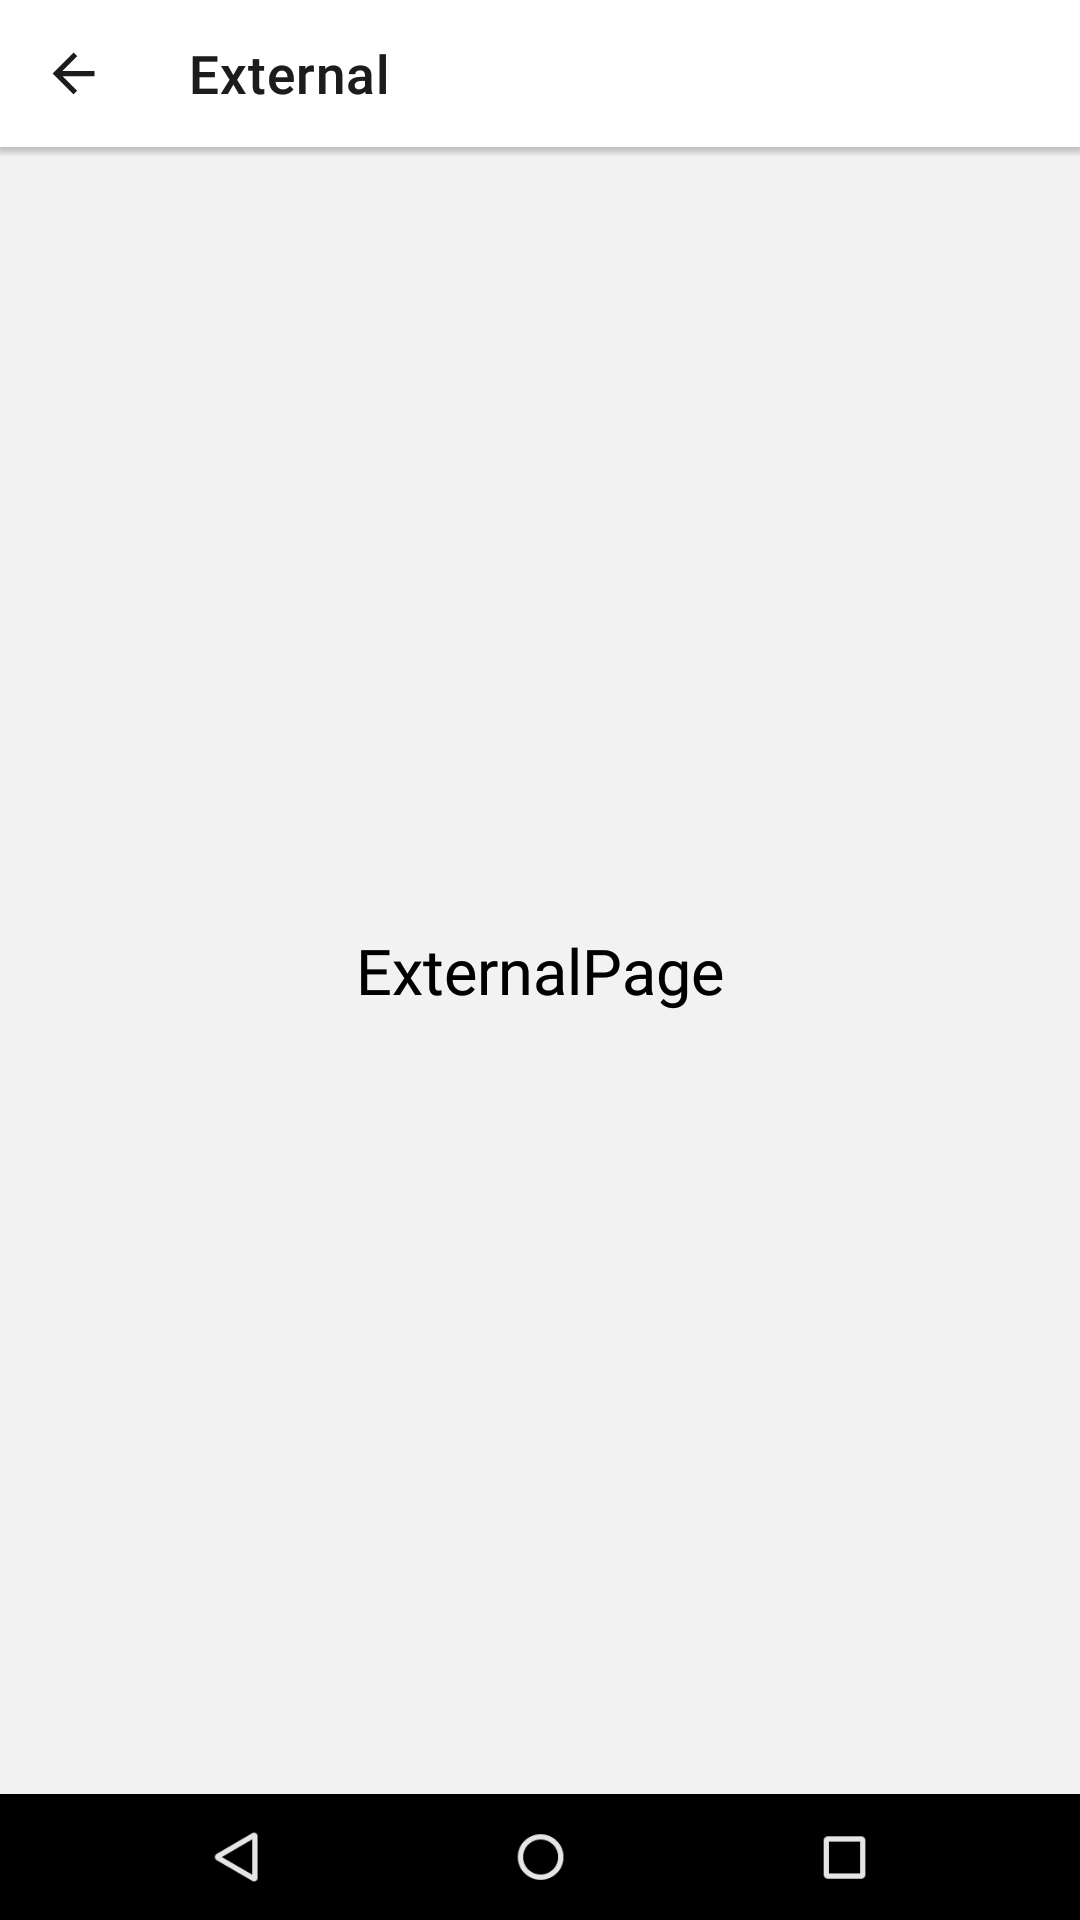
\includegraphics[height=50mm]{img/app4_2_rn_android}
    \caption{App 4 (2/3): React Native Android (Source: Own work)}
    \label{fig:app4_2_rn_android}
  \end{minipage}
  \hfill
  \begin{minipage}{.31\textwidth}
    \centering
    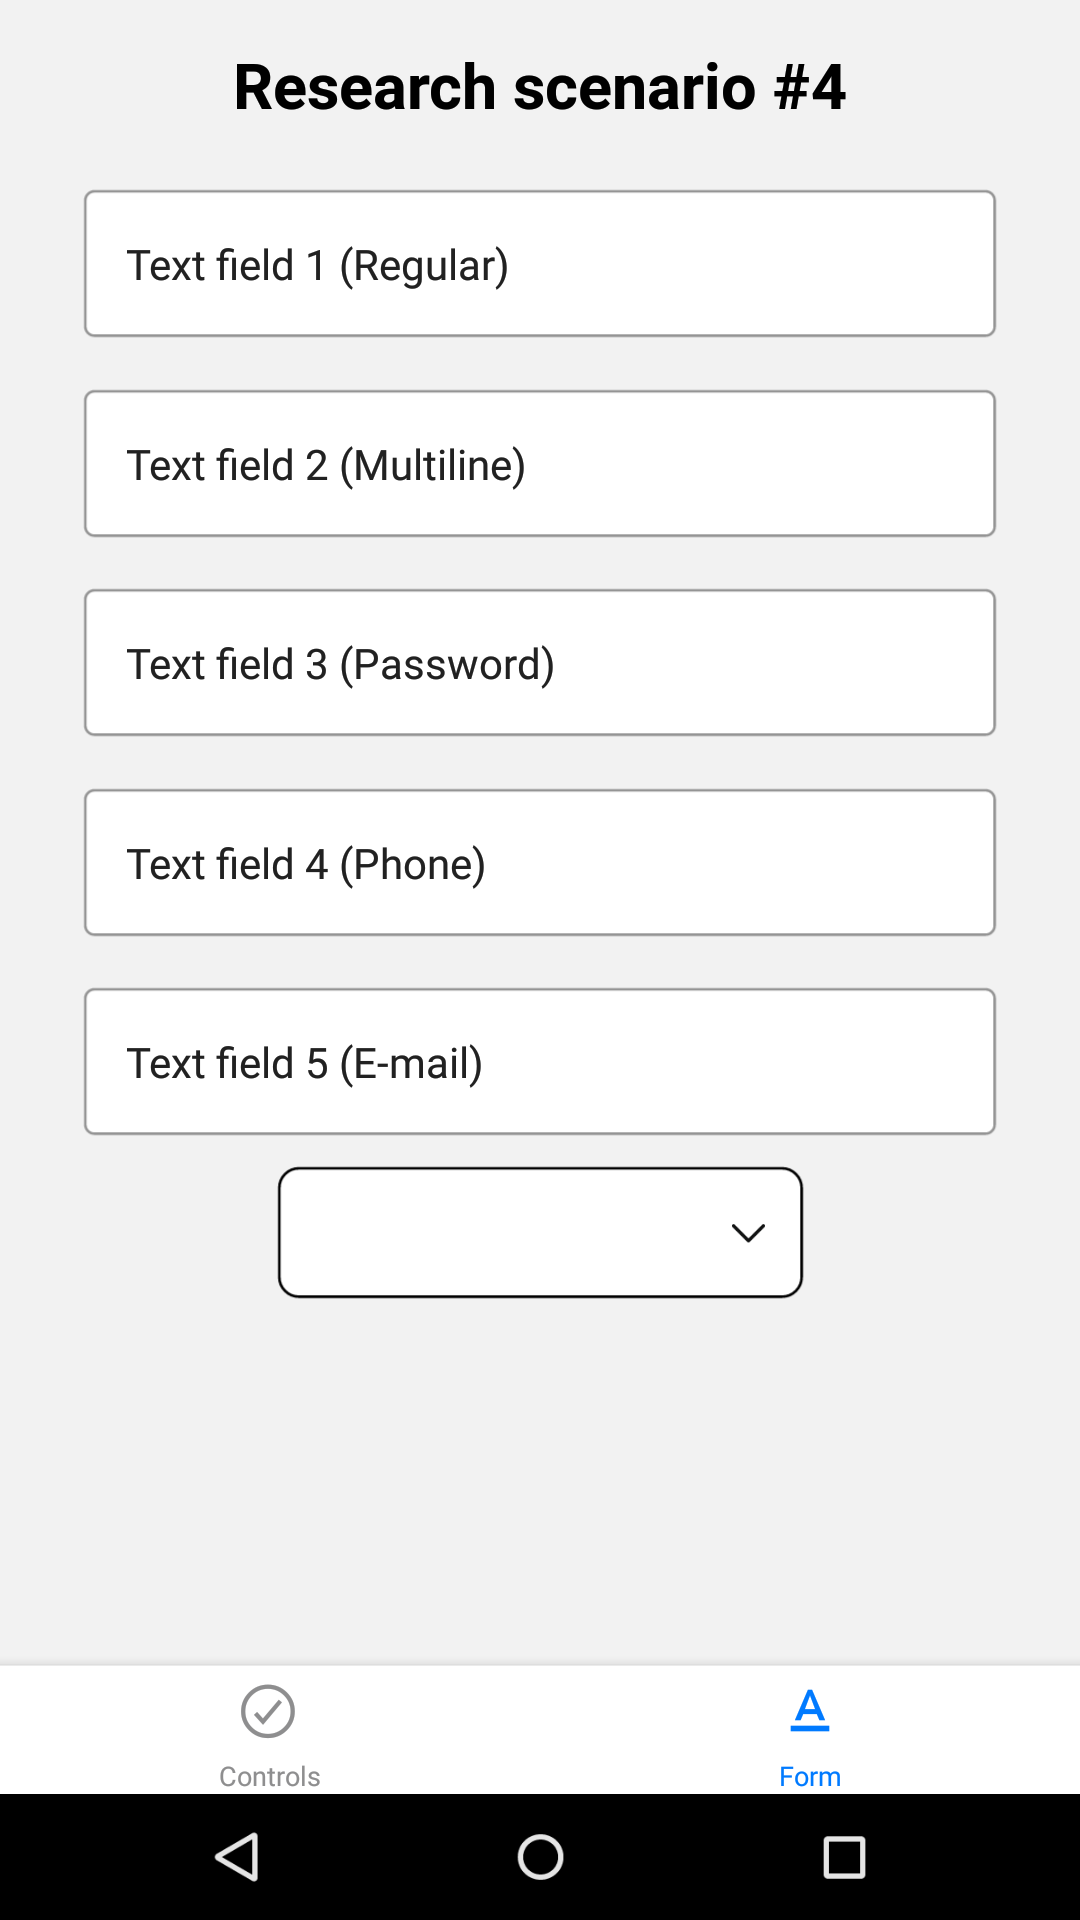
\includegraphics[height=50mm]{img/app4_3_rn_android}
    \caption{App 4 (3/3): React Native Android (Source: Own work)}
    \label{fig:app4_3_rn_android}
  \end{minipage}
\end{figure}

\begin{figure}[H]
  \begin{minipage}{.31\textwidth}
    \centering
    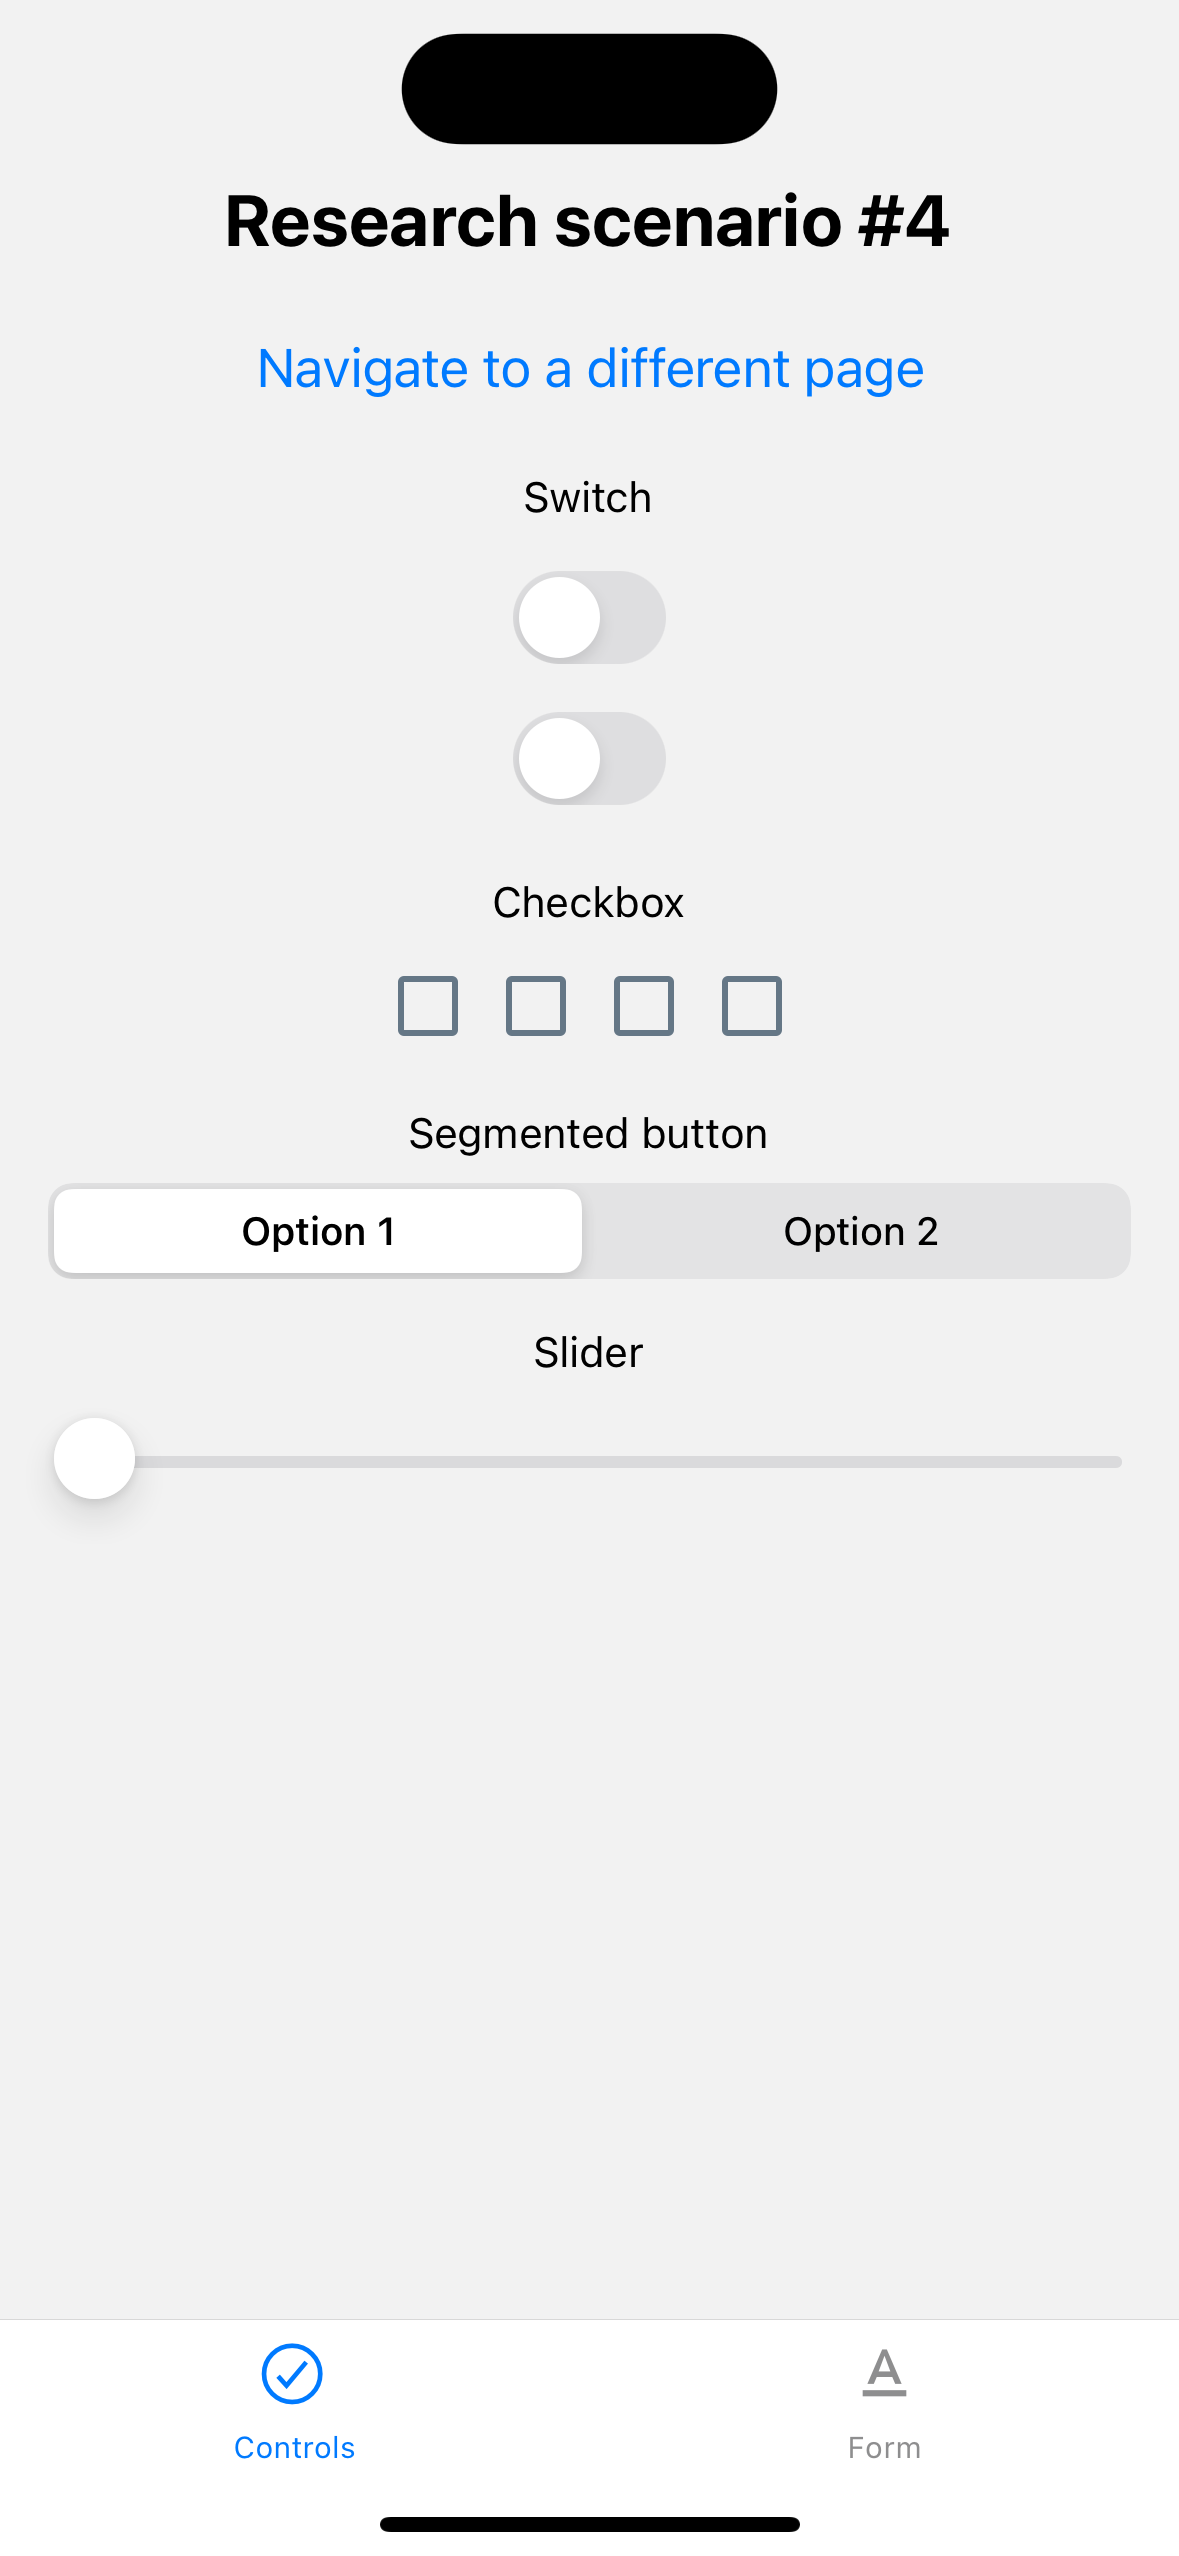
\includegraphics[height=50mm]{img/app4_1_rn_ios}
    \caption{App 4 (1/3): React Native iOS (Source: Own work)}
    \label{fig:app4_1_rn_ios}
  \end{minipage}
  \hfill
  \begin{minipage}{.31\textwidth}
    \centering
    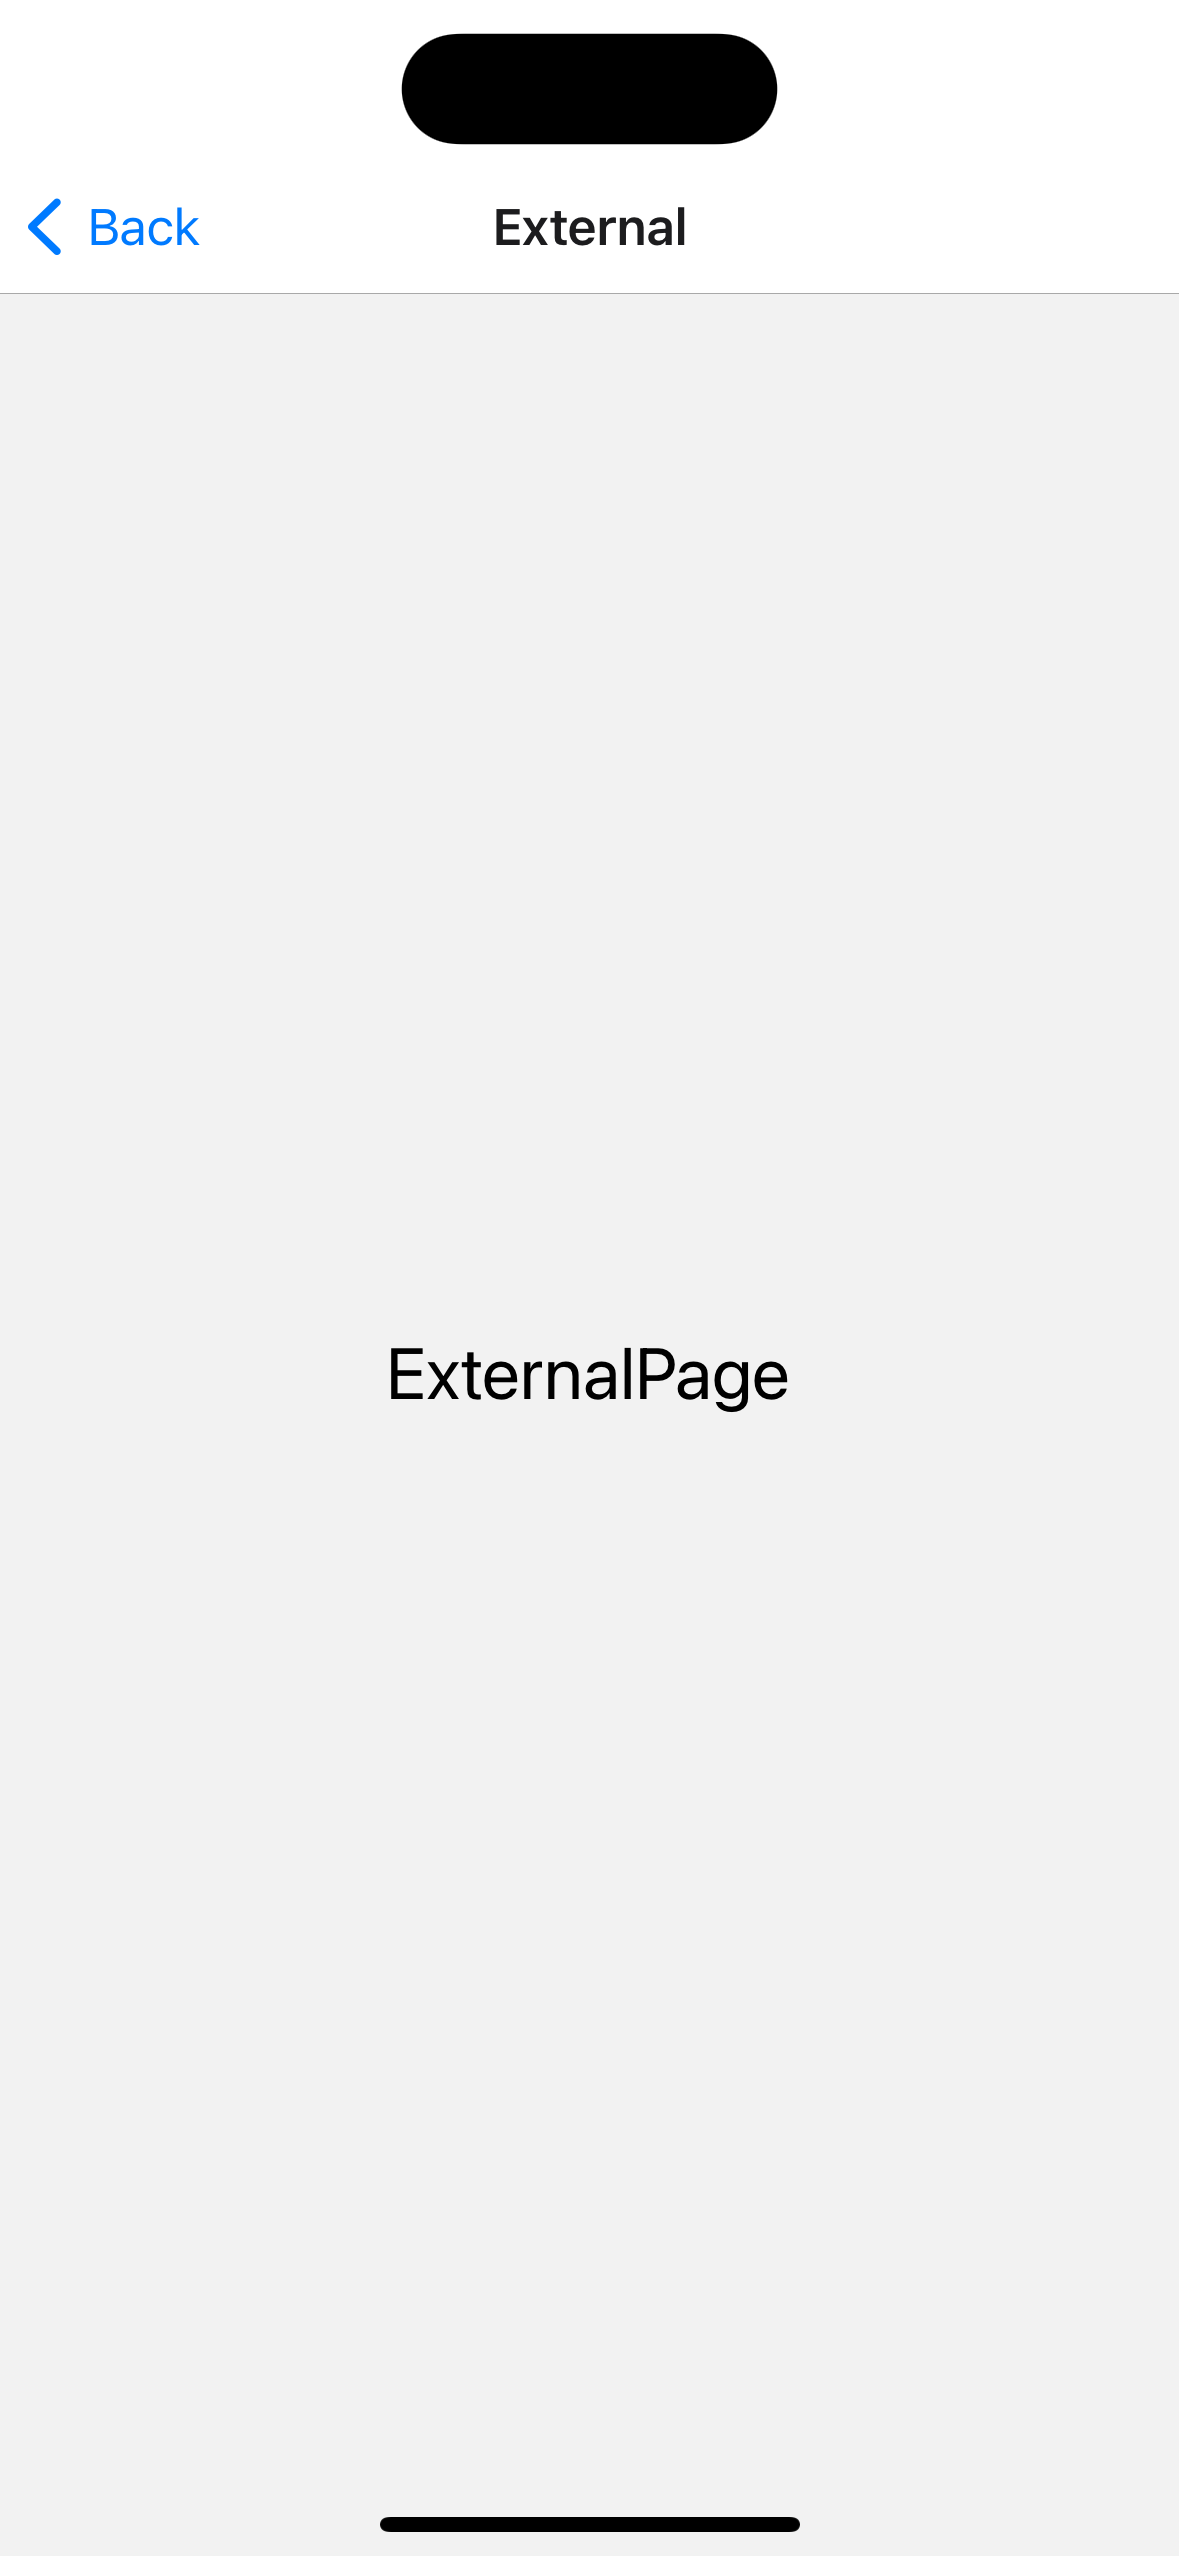
\includegraphics[height=50mm]{img/app4_2_rn_ios}
    \caption{App 4 (2/3): React Native iOS (Source: Own work)}
    \label{fig:app4_2_rn_ios}
  \end{minipage}
  \hfill
  \begin{minipage}{.31\textwidth}
    \centering
    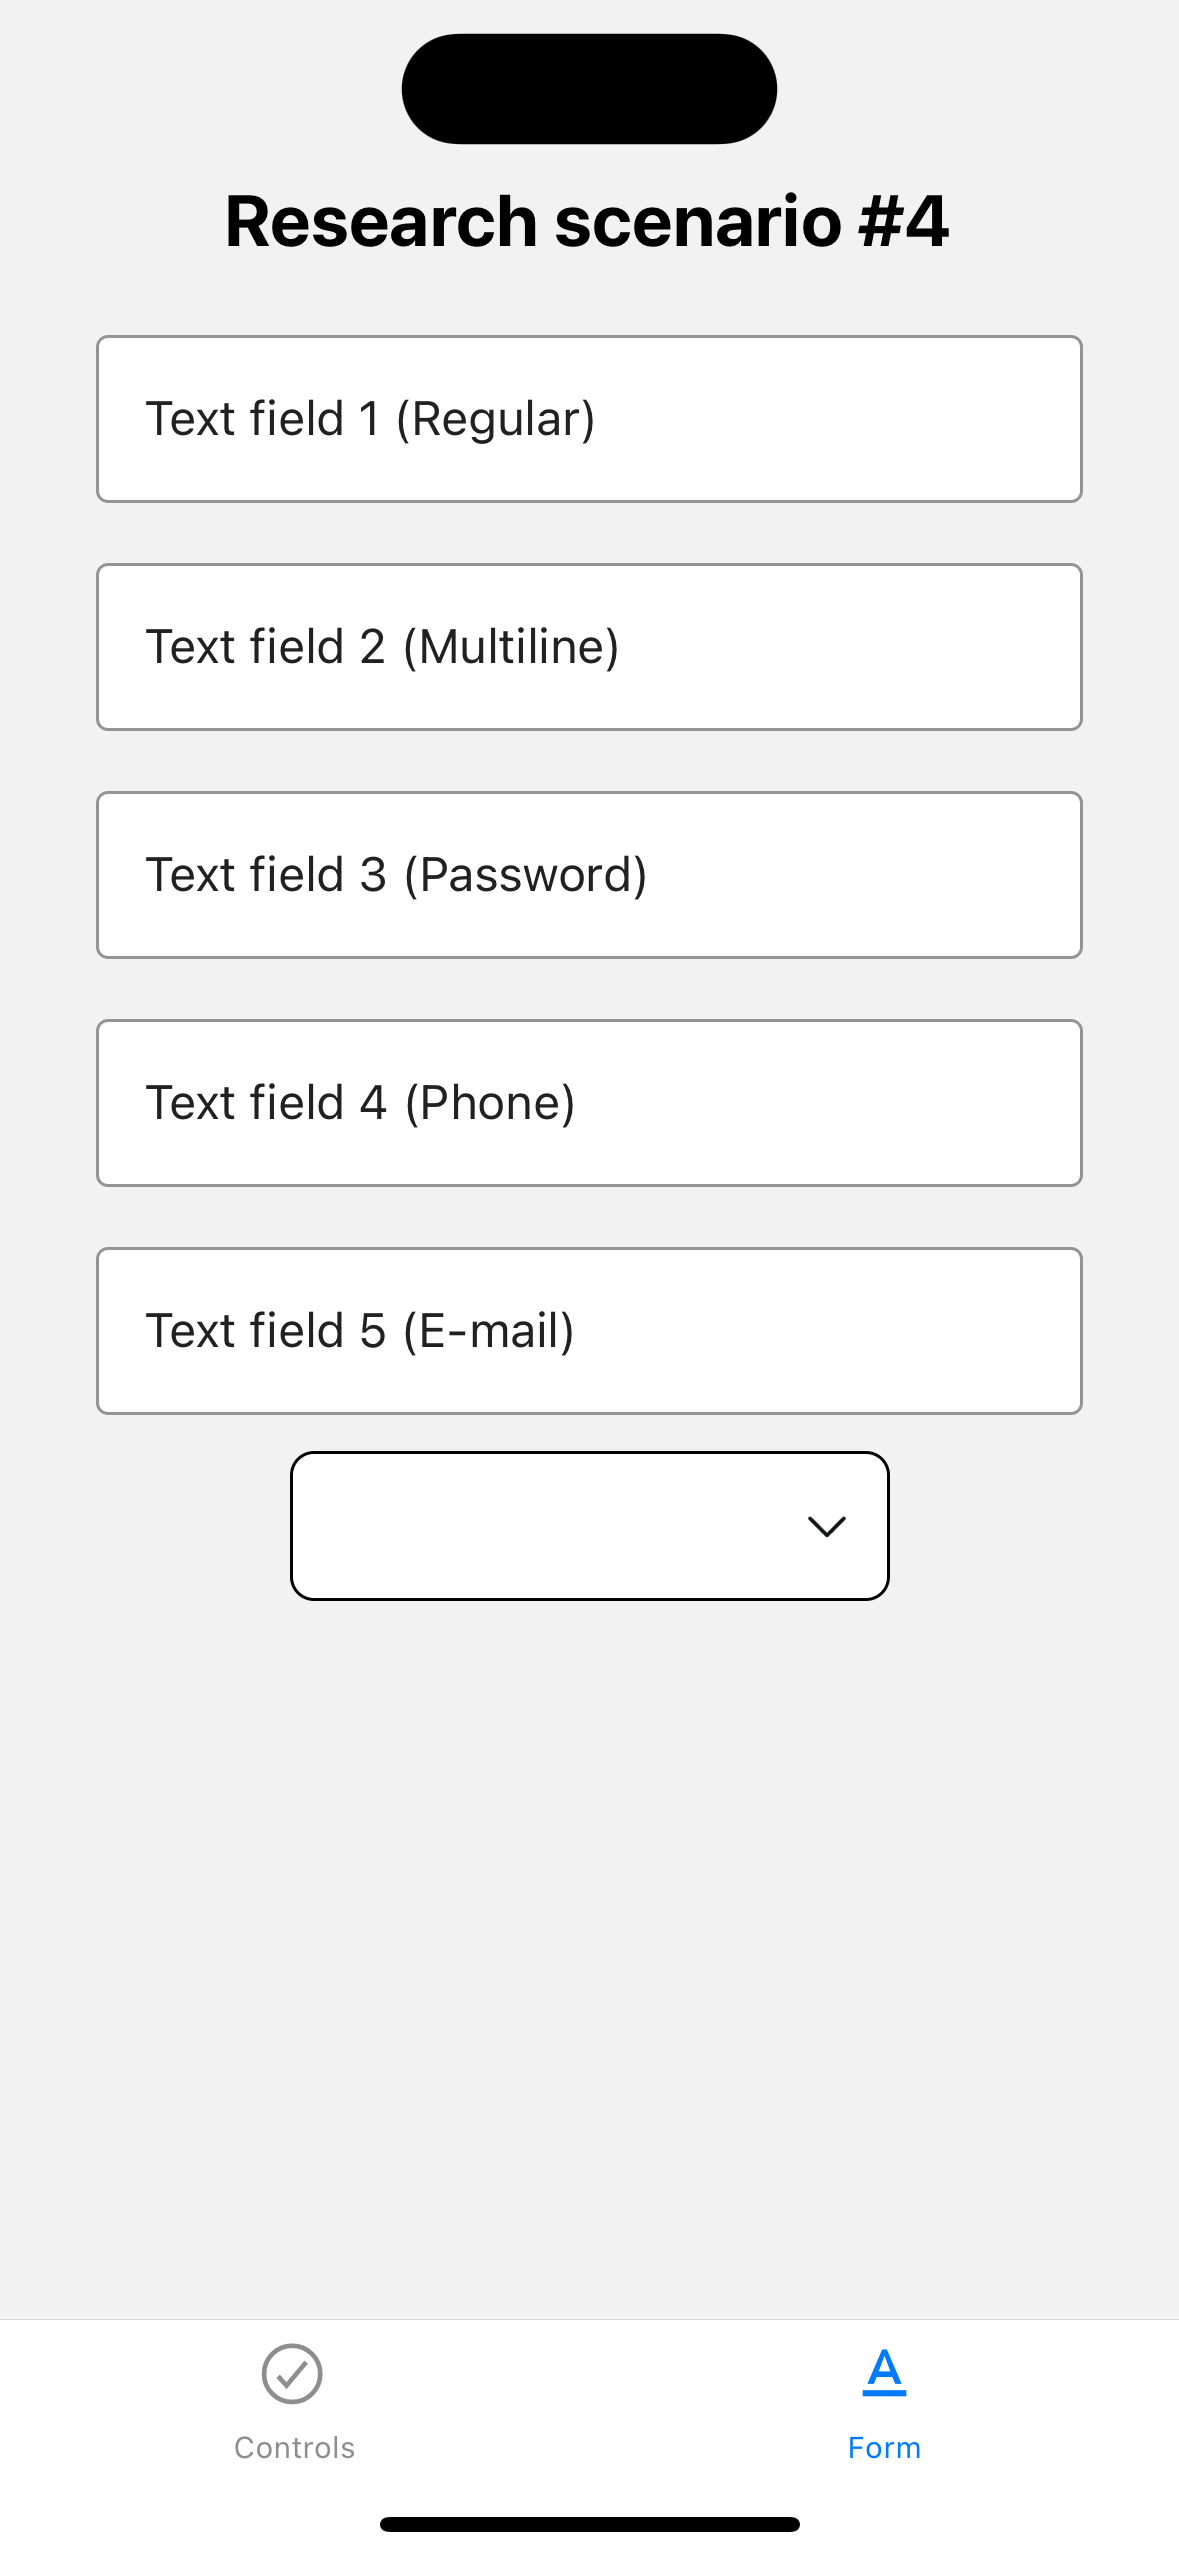
\includegraphics[height=50mm]{img/app4_3_rn_ios}
    \caption{App 4 (3/3): React Native iOS (Source: Own work)}
    \label{fig:app4_3_rn_ios}
  \end{minipage}
\end{figure}

\section{Key takeaways obtained during the implementation process}

As considered in Chapter \ref{chap:cross_mobile_dev}, one of the significant aspects of cross-platform framework development is the ability to acquire the native look and feel of mobile applications. Of course, this does not concern the native approaches. As can be observed in the screenshots above, mobile apps implemented with \emph{Flutter} tend to be almost completely identical to their native equivalents. In case of \emph{React Native}, iOS apps seem to be quite similar, although not as much as in case of \emph{Flutter}. However, a big difference can be noticed when comparing Android apps. The reason for that is that currently \emph{Material Design 3} is the primary design system for user interfaces, and \emph{React Native} has not yet adjusted to it. Moreover, the process of theming is easier in \emph{Flutter} because it is set up for both platforms by default, which is not true for \emph{React Native}. On the other hand, \emph{Flutter} requires more code in order to accomplish this native look and feel. For example, \mintinline{dart}{TextField} and \mintinline{dart}{CupertinoTextField} widgets should be used for Android and iOS respectively for this purpose. This usually is achieved by creating custom widgets, e.g. \mintinline{dart}{MyCustomTextField} which renders the correct widget according to the running operating system and removes the neccessity to check the platform each time a text field is used across the whole application.

During the implementation, the official documentation as well as the community posts could be used as main sources of knowledge. The development process carried out for the purpose of this thesis provided information for the comparison regarding this context. Both \emph{SwiftUI} and \emph{Flutter} offer the most extensible documentation which enables quick understanding of new concepts. Next in line is \emph{React Native} which provides less detailed description of some aspects but still is not lacking. Finally, \emph{Jetpack Compose} documentation comes across as the most general which can result in the neccessity of further research in order to gather enough knowledge for implementation of a specific component.

\clearpage


% !TEX encoding = UTF-8 Unicode 
% !TEX root = praca.tex

\chapter{Summary}

\section{Contribution}

\section{Limitations}

\section{Suggestions for future work}



\bibliographystyle{dyplom}
\bibliography{bibliography}

\listoffigures
\listoftables

\end{document}
